\chapter{ND280 fits}
\label{chap:ND280}

\section{T2K}
The T2K experiment

\section{ND280}
Describe me

\section{Super-Kamiokande}

\section{T2K oscillation analysis chain overview}
The T2K oscillation analyses have a myriad of input groups providing central values and covariances for the systematic parameters. The ND280 beam group provides data on the neutrino beam, the NuMu and Nue systematics and selections groups provide ND280 systematics and suggested binning, the Neutrino Interactions Working Group (NIWG) provide neutrino interaction systematics, and the T2K-SK group provides systematics and selections for SK. Since ND280 and SK are in the same neutrino beam, the high-statistics neutrino samples at ND280 can be used to constrain the simulation prior to seeing data at SK. At the near-detector the flux model, neutrino interaction model and ND280 model is fit. Details on these systematics will be provided in \autoref{subsec:ND280:syst:xsec, subsec:ND280:syst:flux, subsec:ND280:syst:det}. 

T2K has two separate groups fitting near-detector data with the intent of maximising model likelihood: BANFF \red{INSERT ACRONYM} and MaCh3 \red{INSERT ACRONYM}. The two frameworks use identical event selections and systematic parameters, outlined below in \autoref{subsec:ND280:sel} and \autoref{subsec:ND280:syst}, but entirely different methods of evaluating the model goodness and exploring the parameter space.

BANFF interfaces to the popular gradient-descent minimizer MINUIT \red{CITE} and MaCh3 uses a custom Markov Chain Monte Carlo sampler to sample the high dimensional parameter space. Importantly, the BANFF attempts to find the global minimum of the test-statistic given the data and the model, whereas MaCh3 explores an area around the minimum test-statistic with the intent of sampling the Bayesian posterior. Therefore, MaCh3 does not necessarily locate a set of ``best-fit'' parameters with covariances assuming a parabolic minimum: instead it provides a full high-dimensional posterior with arbitrary shape. Once the model is constrained by near-detector data, the T2K oscillation analysis chain can then proceed using the model proposed by the near-detector data and model and include oscillation effects.

However, providing a high-dimensional posterior of arbitrary shape is cumbersome, so oscillation groups often use the BANFF output. MaCh3 has the advantage of a near and far detector implementation, meaning a simultaneous fit of data from both detectors can be done. This avoids assumptions on the underlying probability distribution functions of the parameters and the likelihood surface, and additionally benefits from fully correlating the models at both detectors, allowing one to affect the other as the fit proceeds.

The following sections detail the near-detector implementation of the MaCh3 framework. It also includes comparisons and validations to the BANFF framework. It finishes with the 2017 round fit to data.

\section{Need for ND280 fits}
As statistics increase at Super-Kamiokande, there is more and more need for well-controlled systematics. The T2K oscillation analysis uses \red{CITEME}

SK without constraints
Share same beam, use near detector complex

\section{Selections}
\label{sec:ND280:sel}
The goal of the selection is to map theory interaction modes (e.g. CCQE, CC1$\pi^+$, CC DIS) to ND280 selections, so that theory parameters receive largest constraints from fewest exclusive samples. Equivalent FGD1 and FGD2 selections are separated due to differences in systematics and reconstruction: forward-going tracks emanating in FGD1 leaves a track in FGD1, TPC2, FGD2 and TPC3 so has more hits recorded than the FGD2 equivalence, which only passes through FGD2 and TPC3. Furthermore, FGD2 contains plastic scintillator interleaved with passive water layers whereas FGD1 is fully plastic scintillator. Separating FGD1 and FGD2 also allows constraints on water interactions to come strictly from the FGD2 selections.

The fit bins events in the two reconstructed muon variables \pmu and \cosmu. The muon variables are chosen primarily due to excellent detector resolution of muons and because this is what T2K oscillation analyses observe at \sk. There is ongoing effort to bin in pion variables when such are present (e.g. for CC$1\pi^+$ or CCOther selections), and composite variables in the plane transverse to the neutrino, but these will not be presented here.

The selections are entirely defined by the observed reconstructed event topology of an event in the detector and there is no attempt at correcting for misidentified particles. There is also no attempt to correct for nuclear effects such as final-state-interactions.
\begin{itemize}
\item \textbf{CC$0\pi$}: Events with one negative muon without any charged or neutral pions in the final state. It is developed to contain CCQE and 2p2h events and is the largest sample at ND280. An example event display is shown in \autoref{fig:cc0pi_evtdisplay}. \red{show plots of cross-sections at ND280 from NEUT?}
\begin{figure}[htbp]
	\begin{subfigure}[t]{0.49\textwidth}
		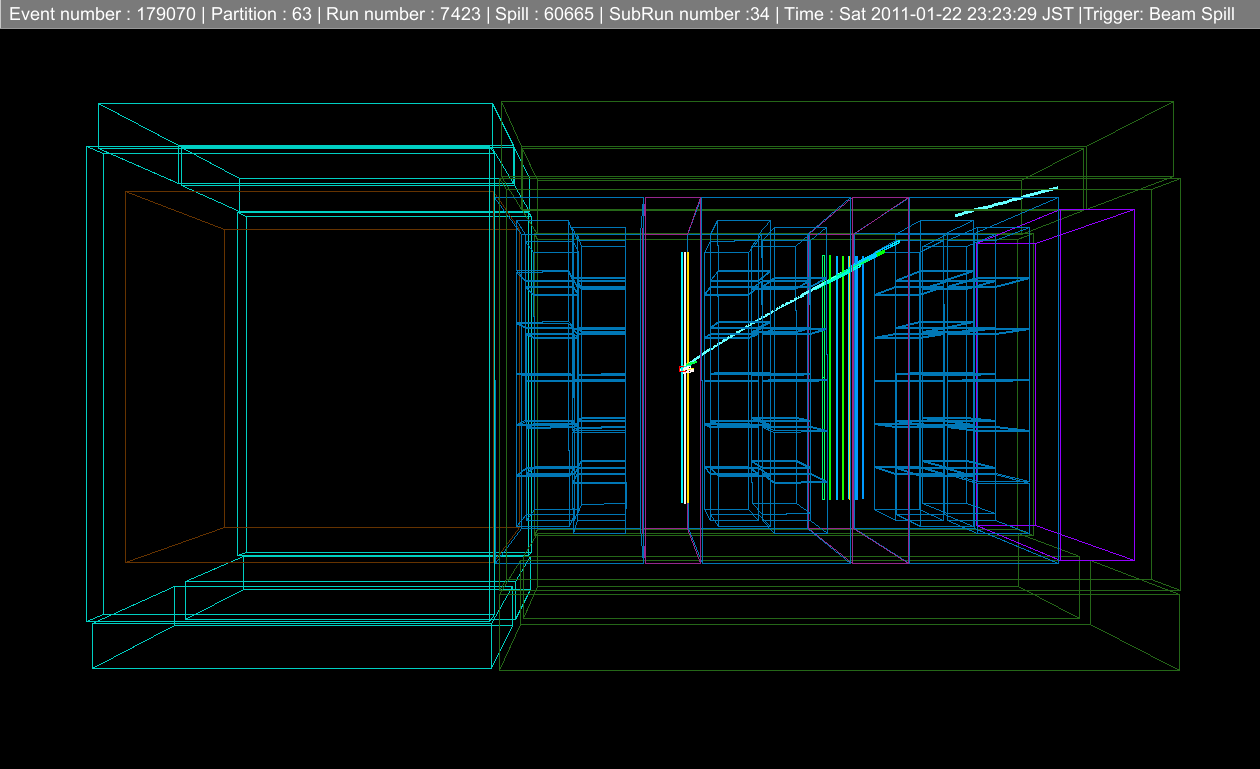
\includegraphics[width=\textwidth, trim={1cm 2.8cm 0 1cm}, clip]{figures/numu/evtdisplay/CC0pi_7423_34_179070_perX0Z_all}
		\caption{Side-view}
	\end{subfigure}
	\begin{subfigure}[t]{0.49\textwidth}
		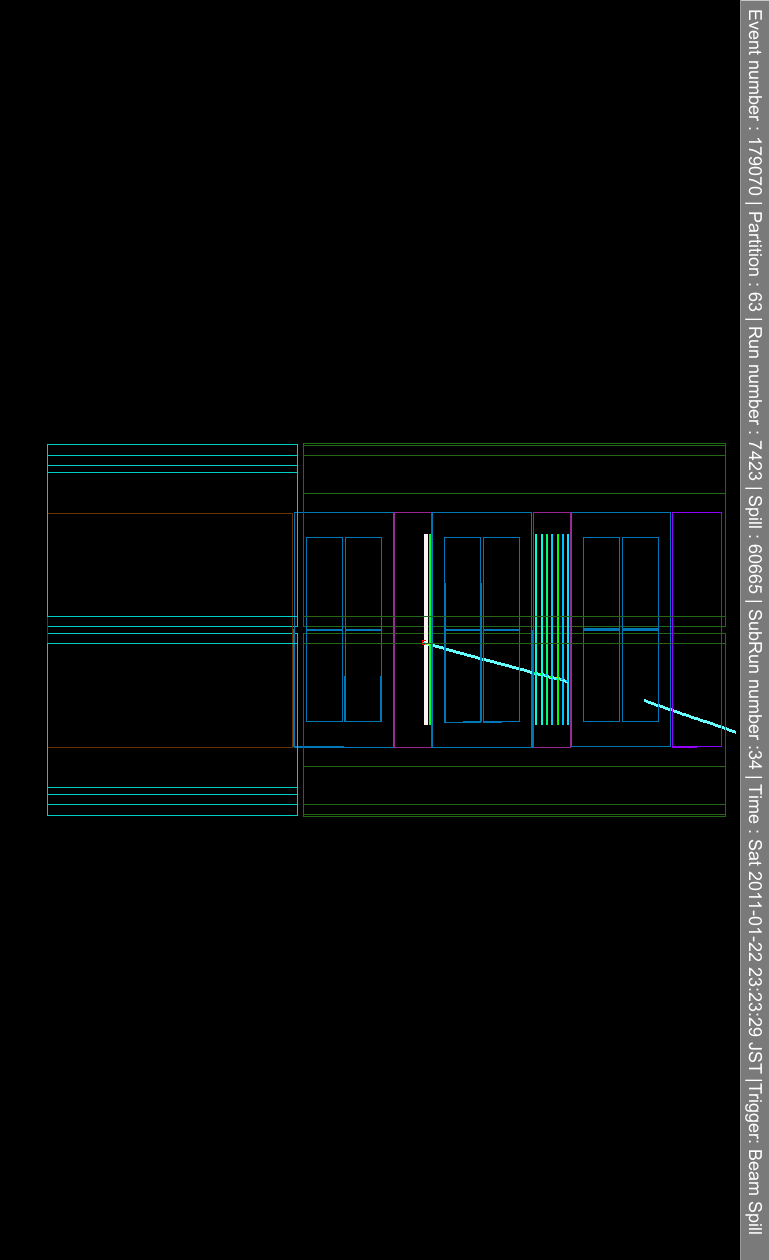
\includegraphics[width=\textwidth, trim={1cm 15cm 1cm 15cm}, clip]{figures/numu/evtdisplay/CC0pi_7423_34_179070_ortX0Z_all}
	\caption{Top-view}
	\end{subfigure}
	\caption{True FGD1 CC0$\pi$ event display in ND280}
	\label{fig:cc0pi_evtdisplay}
\end{figure}

\item \textbf{CC$1\pi$}: Events with one negative muon and one positive pion with no negative or neutral pions in the final state. It is developed to contain mostly CC1$\pi^{+}$ events from resonant interactions\red{refer to previous sections maybe}. An example event display is shown in \autoref{fig:cc1pi_evtdisplay}. 
\begin{figure}[htbp]
	\begin{subfigure}[t]{0.49\textwidth}
		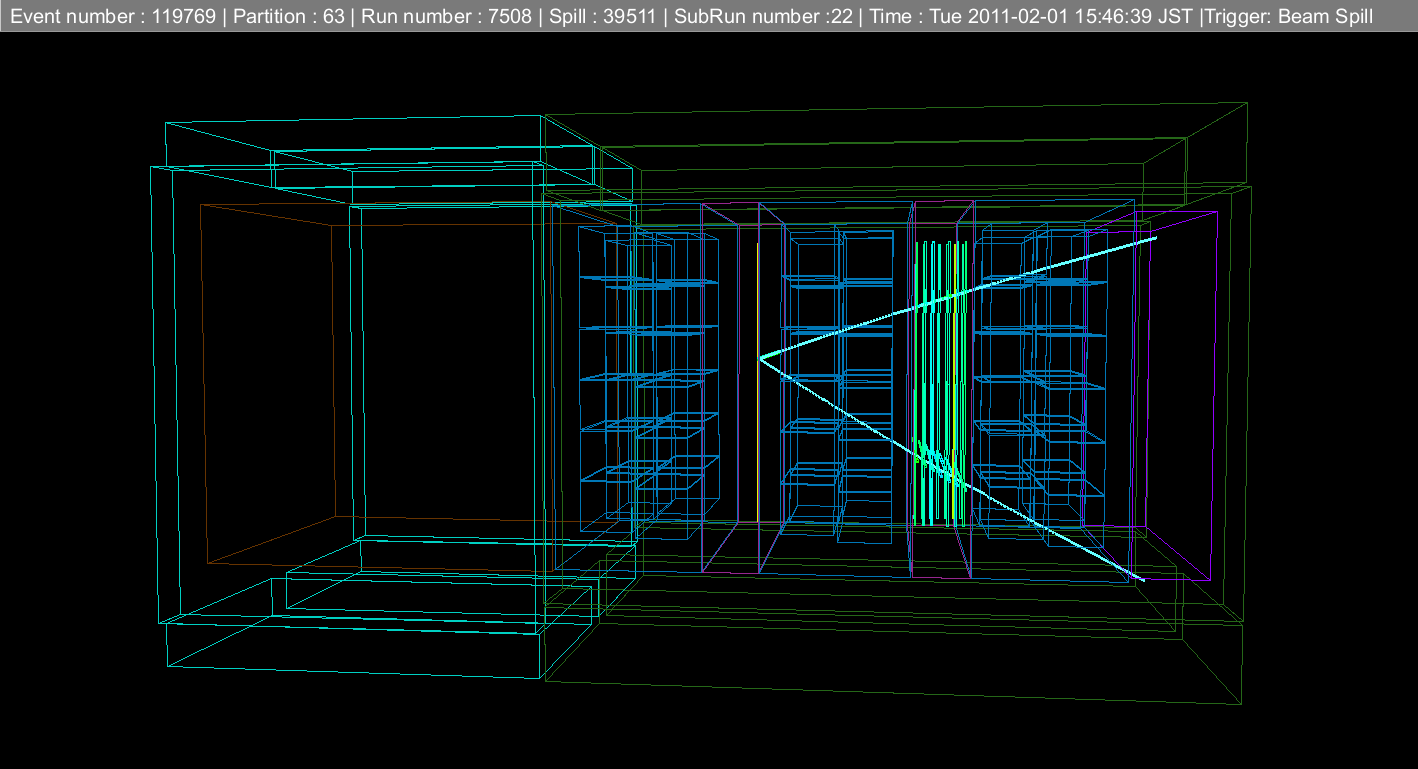
\includegraphics[width=\textwidth, trim={4cm 2cm 4cm 3cm}, clip]{figures/numu/evtdisplay/CC1pi_7508_22_119769_perpX0Z_all}
		\caption{Side-view}
	\end{subfigure}
	\begin{subfigure}[t]{0.49\textwidth}
		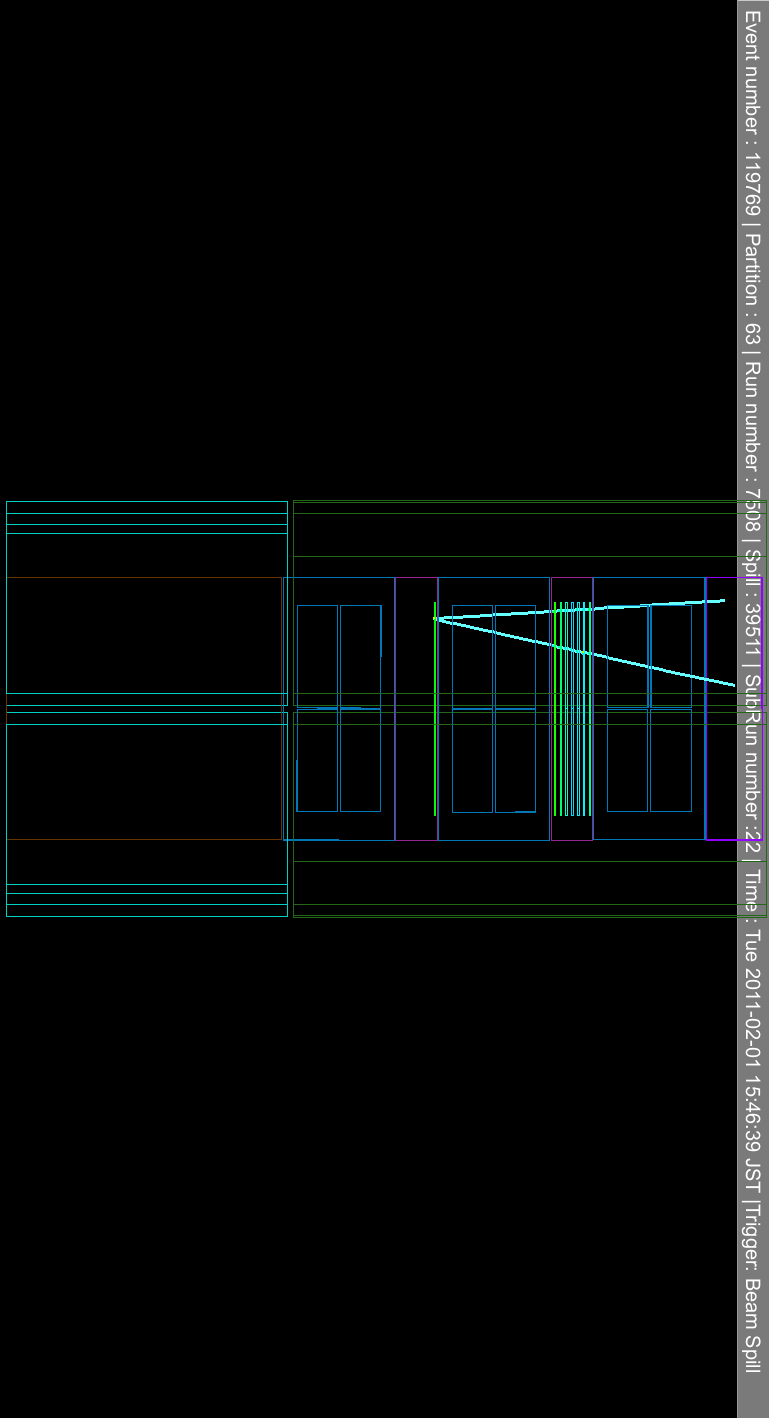
\includegraphics[width=\textwidth, trim={0cm 17cm 1cm 17cm}, clip]{figures/numu/evtdisplay/CC1pi_7508_22_119769_ortX0Z_all}
		\caption{Top-view}
	\end{subfigure}
	\caption{True FGD1 CC1$\pi$ event display in ND280}
	\label{fig:cc1pi_evtdisplay}
\end{figure}

\item \textbf{CC Other}: Events with one negative muon and any number of neutral or negative pions which does not satisfy CC1$\pi$ selection. The presence of one $\pi^{-,0}$ or more than one $\pi^+$ in an event makes this possible. There are no constraints on the number of reconstructed heavier mesons (e.g. kaons or etas). It is developed to contain mostly DIS interactions and CC$1\pi^0$. An example event display is shown in \autoref{fig:ccoth_evtdisplay}.
\end{itemize}
\begin{figure}[htbp]
	\begin{subfigure}[t]{0.49\textwidth}
		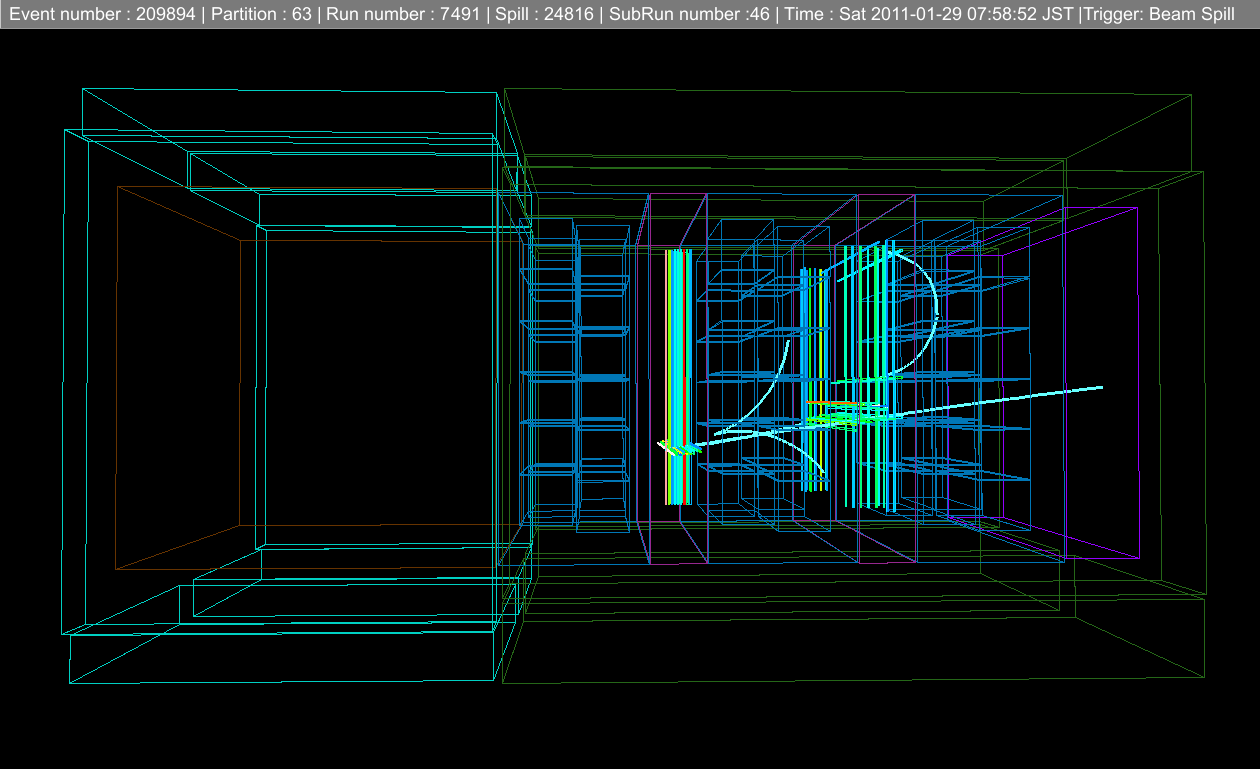
\includegraphics[width=\textwidth, trim={1cm 3cm 1cm 1cm}, clip ]{figures/numu/evtdisplay/CCOthers_7491_46_209894_perX0Z_all}
		\caption{Side-view}
	\end{subfigure}
	\begin{subfigure}[t]{0.49\textwidth}
		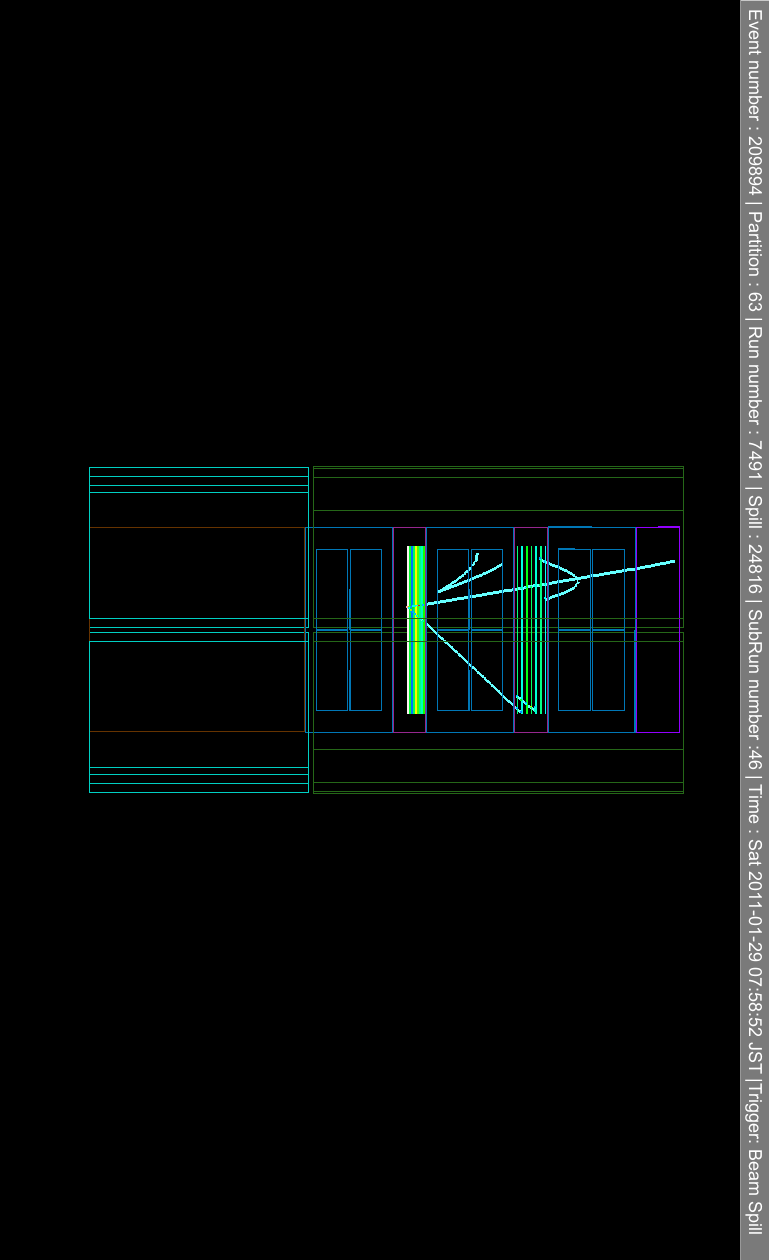
\includegraphics[width=\textwidth, trim={3cm 16cm 3cm 16cm}, clip]{figures/numu/evtdisplay/CCOthers_7491_46_209894_ortX0Z_all}
		\caption{Top-view}
	\end{subfigure}
	\caption{True FGD1 CCOther event display in ND280}
	\label{fig:ccoth_evtdisplay}
\end{figure}

\subsection{Event selection cuts, \numu}
\label{sec:numu_sel}
The different topological selections all start by isolating CC-inclusive candidates in FGD1 or FGD2. Firstly is required to contain one reconstructed track candidate of negative charge crossing the TPC downstream of either FGD (TPC2 for interactions starting in FGD1, TPC3 for interactions starting in FGD2). The event also needs to fulfil data quality and fiducial volume requirements. The muon is then assumed to be the highest momentum negative track (HMNT) found in the event, and it is required that the track is identified as a muon.

The detailed general selection criteria for the CC-inclusive sample is:
\begin{itemize}
	\item \textbf{Event quality cut}: The full beam spill has a good global ND280 data quality flag, meaning all ND280 sub-detectors and magnet were operational and reading out data. The event must occur within the bunch time window of the neutrino beam. Event pile-up is mitigated by associating each event to a beam bunch within a beam spill.
	
	\item \textbf{Quality and fiducial volume cut}: At least one reconstructed track is present in the FGD1 or FGD2 fiducial volume. The fiducial volume for FGD1 is $|x|<874.51\text{ mm}$, $|y-55|<874.51\text{ mm}$, $136.875 < z < 446.955\text{ mm}$ and for FGD2 $|x|<874.51\text{ mm}$, $|y-55|<874.51\text{ mm}$, $1481.45< z < 1807.05\text{ mm}$\footnote{The 55mm offset in $y$ reflects the shift in XY modules relative the center of the ND280 coordinate system.}.
	
	The $x$ and $y$ cuts are designed to accept interactions which have their vertex five bars from the edge of the XY module of each FGD. The $z$ cut excludes the first XY module of each FGD and includes the remaining (14 for FGD1, 7 for FGD2). To reject short tracks, for which the TPC reconstruction is unreliable, tracks are required to have more than 18 TPC clusters.
	
	\item \textbf{Upstream background veto}: If the second highest momentum track starts at least 150 mm upstream of the selected muon candidate (highest momentum negative track with muon PID), the event is rejected. This cut eliminates events in which the muon candidate might be the second part of a broken track which started further upstream (e.g. in the P0D). For events with a reconstructed vertex in FGD2 there is the added criterion of having no reconstructed tracks in FGD1.
	
	\item \textbf{Broken track cut}: The start position of the muon candidate track needs to be less than 425 mm away from the FGD upstream edge if the event has at least one reconstructed FGD-only track. The cut vetoes events where the reconstruction has cut a muon candidate track into two tracks: one of which is fully contained in the FGD and the second starting downstream of the fully contained track in the FGD and enters the TPC, causing the second track to be the selected as the muon candidate, misplacing the vertex.
	
	\item \textbf{Muon PID cut}: Once a particle is considered a muon candidate (fulfilling the above criteria), the particle identification is applied based on the observed $dE/dx$ measurement of the track in the TPC. The measured energy deposit $E$ in the TPC is compared with the expected energy deposit under muon, pion, electron and proton hypotheses and pulls and discrimination functions are then applied.
	
	The pulls $\delta_i$ for particle type $i$ are defined as
	\begin{equation}
	\label{eq:tpc_track_chi2}
	\delta_i = \frac{C_T^{obs}-C_T^{exp}}{\sigma^{exp}}
	\end{equation}
	where the expected energy loss $C_T^{exp}$ is parameterised as
	\begin{equation}
	C_T^{exp} = \frac{53.87 \text{ ADC}}{\beta^{2.283}} \left( 5.551 - \beta^{2.283} - \log\left[0.001913 + \frac{1}{\left(\beta\gamma\right)^{1.249}}\right]\right)
	\end{equation}
	and $\sigma^{exp}$ is the deposited energy resolution of the TPC.
	
	The likelihoods $\mathcal{L}_i$ are then defined as
	\begin{equation}
	\label{eq:tpc_track_likelihood}
		\mathcal{L}_i = \frac{e^{-\delta^2_i}}{\sum_n e^{-\delta^2_n}}
	\end{equation}
	where the denominator is over $n$, which are the particles $n=\mu,\pi,e,p$. 
	
	In the PID algorithm, electrons are rejected by requiring
	\begin{equation}
		\label{eq:tpc_track_mip}
		\mathcal{L}_{MIP} = \frac{\mathcal{L}_\mu + \mathcal{L}_\pi}{1-\mathcal{L}_p} > 0.8
	\end{equation}
	for tracks with $p<500\text{ MeV/c}$. To remove protons and pions, it is required that
	\begin{equation}
	\label{eq:tpc_track_mu}
		\mathcal{L}_\mu > 0.05
	\end{equation}
	The constants 0.8, 0.05 and 500 MeV/c are chosen from particle gun studies in the TPC and test-beam data, and the impact on the selection is shown in \autoref{fig:numu_likelihoods}. The TPC pulls after preselection are shown in \autoref{fig:numu_pulls}, and the energy loss in the TPC from which pulls are derived are shown in \autoref{fig:TPC_dedx}.
	
	Importantly, TPC segments need to pass the TPC track quality cut contribute to the likelihood: bad quality tracks do not. If a track passes through multiple TPCs all TPC tracks are taken into account.
\end{itemize}

\begin{figure}[!h]
	\begin{subfigure}[t]{0.49\textwidth}
		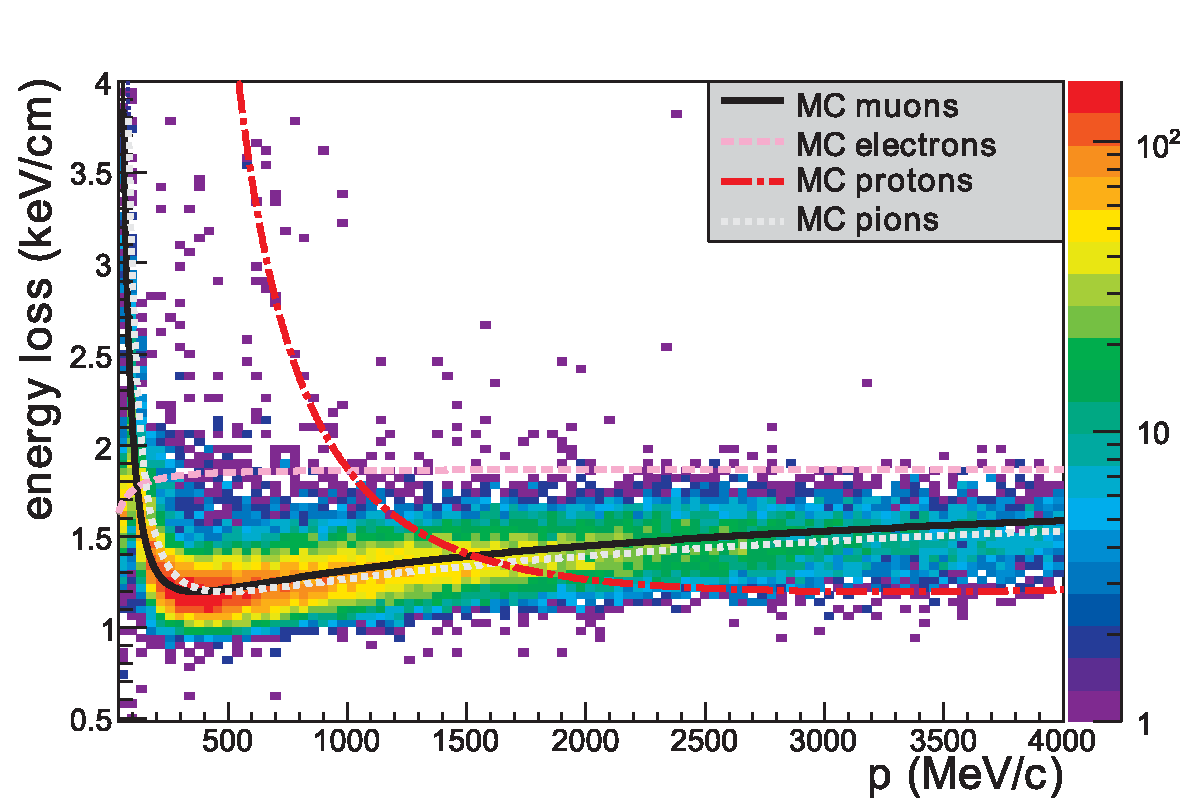
\includegraphics[width=\textwidth]{figures/numu/TPC_PID_neg}
		\caption{Negative particles}
	\end{subfigure}
	\begin{subfigure}[t]{0.49\textwidth}
		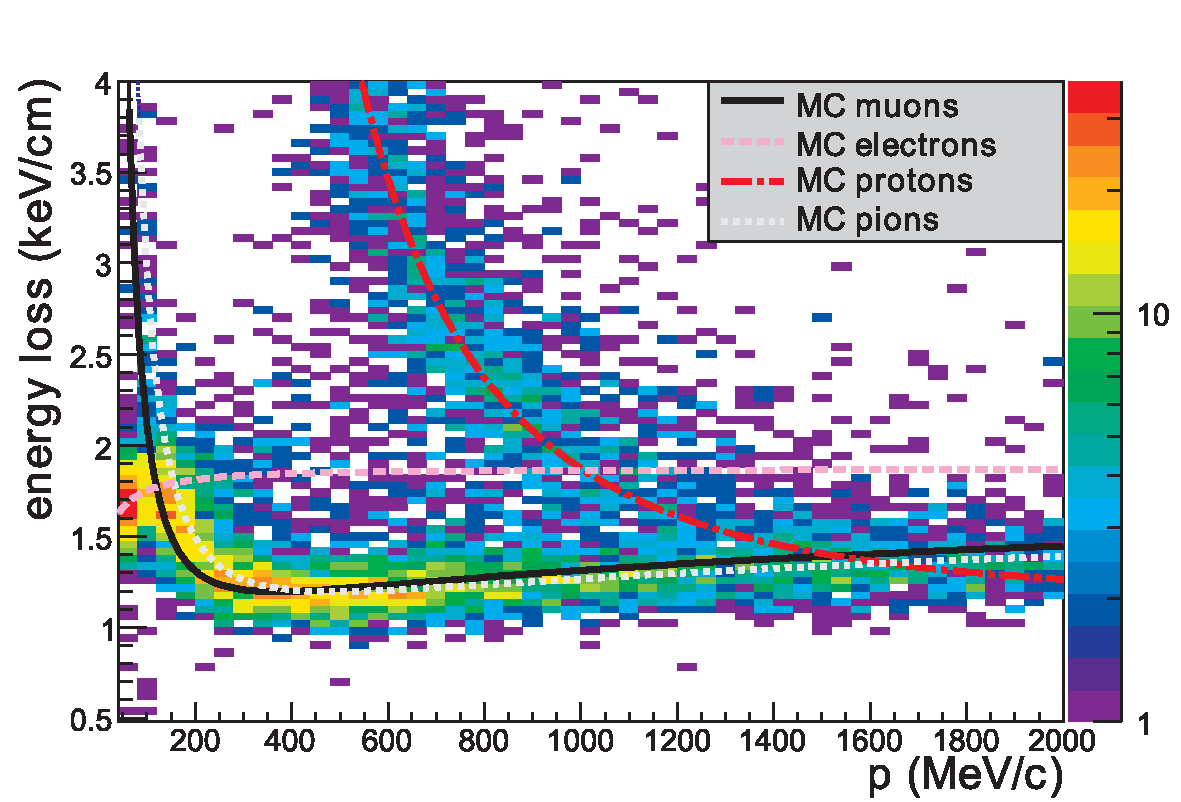
\includegraphics[width=\textwidth]{figures/numu/TPC_PID_pos}
		\caption{Positive particles}
	\end{subfigure}
	\caption{The energy loss for particles travelling through the TPC}
	\label{fig:TPC_dedx}
\end{figure}

\begin{figure}[!h]
	\begin{subfigure}[t]{0.49\textwidth}	
		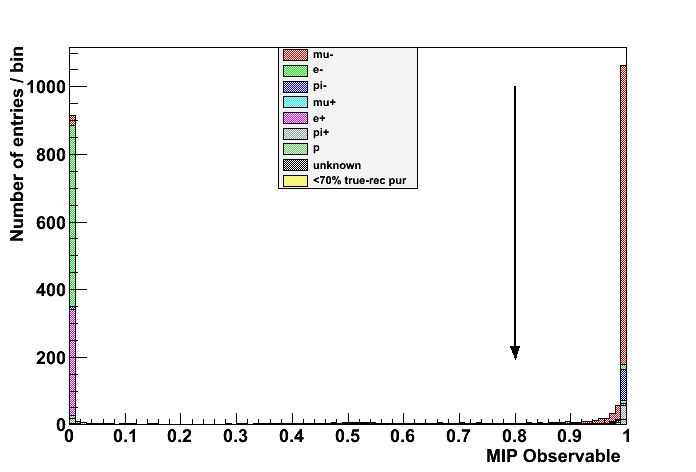
\includegraphics[width=\textwidth]{figures/numu/Cuts/numu/Miplik_run12}
		\caption{$\mathcal{L}_{MIP}$}
	\end{subfigure}
	\begin{subfigure}[t]{0.49\textwidth}	
		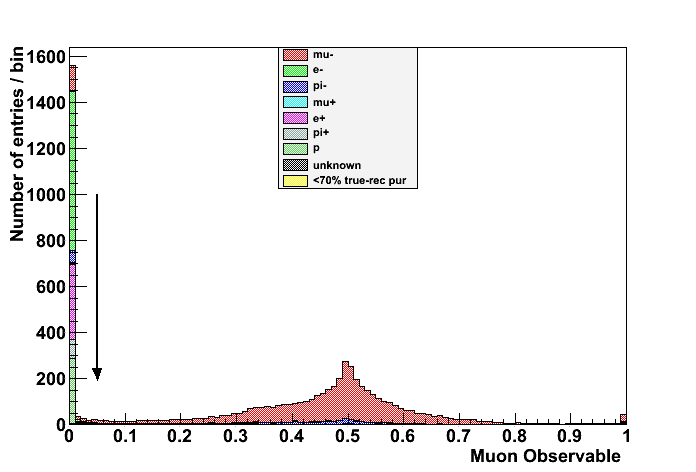
\includegraphics[width=\textwidth]{figures/numu/Cuts/numu/Mulik_run12}
		\caption{$\mathcal{L}_{\mu}$}
	\end{subfigure}
	\caption{Likelihood distributions for preselected MC events, showing cuts placed for \numu analysis}
	\label{fig:numu_likelihoods}
\end{figure}

\begin{figure}[!h]
	\begin{subfigure}[t]{0.32\textwidth}
		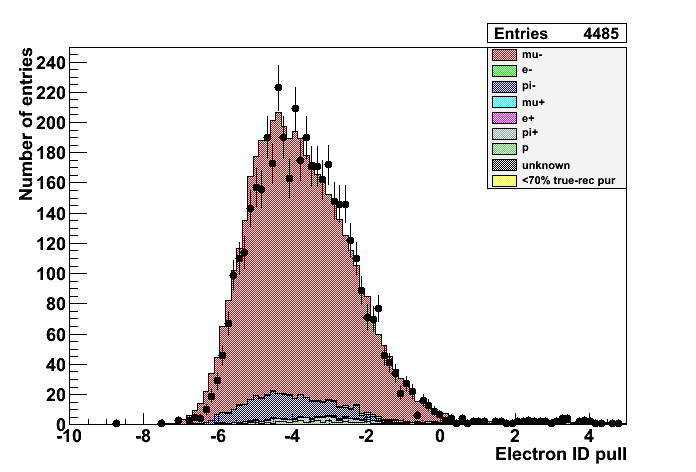
\includegraphics[width=\textwidth]{figures/numu/Cuts/numu/Elepull_run12}
		\caption{$Pull_e$}
	\end{subfigure}
	\begin{subfigure}[t]{0.32\textwidth}	
		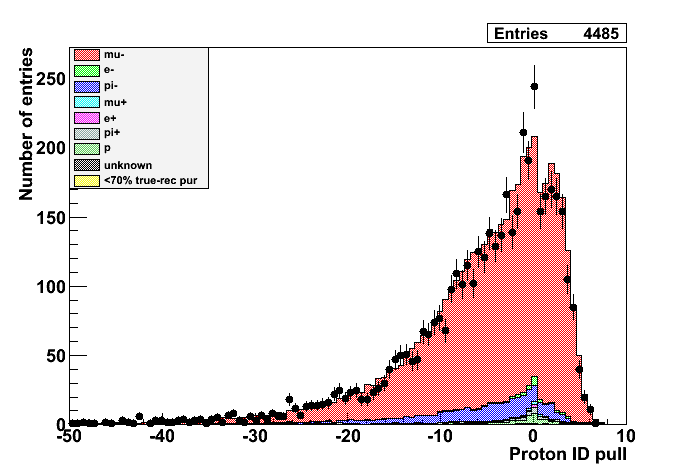
\includegraphics[width=\textwidth]{figures/numu/Cuts/numu/Protpull_run12}
		\caption{$Pull_p$}
	\end{subfigure}
	\begin{subfigure}[t]{0.32\textwidth}
		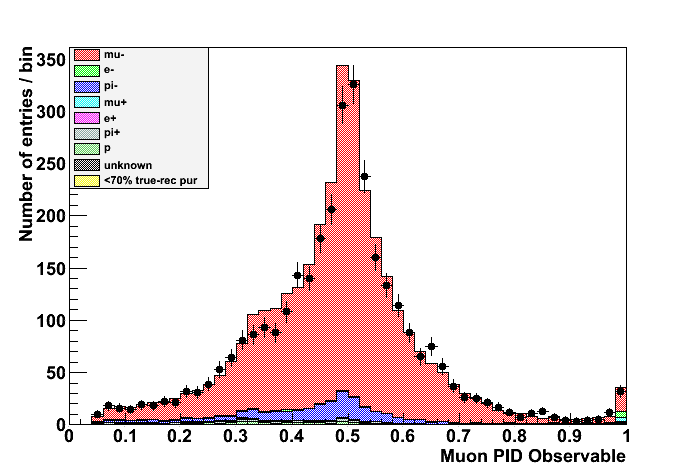
\includegraphics[width=\textwidth]{figures/numu/Cuts/numu/Mulikelihood_run2}
		\caption{$Pull_\mu$}
	\end{subfigure}
	\caption{Pull distributions after selection showing data and MC for \numu analysis}
	\label{fig:numu_pulls}
\end{figure}

The selection criteria then proceeds to split the CC-inclusive sample into the three subsamples: CC$0\pi$, CC$1\pi$ and CCOther. This is based entirely on pion identification in the TPCs and FGDs.

To identify pion candidate(s) a number of cuts are applied:
\begin{itemize}
	\item \textbf{Muon candidate}: The track can not be identified as the above muon candidate.
	
	\item \textbf{Matching beam spill and bunch}: The pion candidate is required to originate from the same beam bunch and spill to the identified muon candidate.
	
	\item \textbf{Track origin}: The pion candidate is required to start in the same FGD fiducial volume as the muon candidate and enter the downstream TPC for PID purposes. The same FGD and TPC track quality and fiducial volume cut is applied for the pion candidate as for the muon candidate.
	
	\item \textbf{Pion PID}: For positive tracks in the TPC, pion, positron and proton hypotheses are tested. For negative tracks, pion and electron hypotheses are tested. 
	
	As for the muon candidate, \autoref{eq:tpc_track_chi2} and \autoref{eq:tpc_track_likelihood} defines the particle likelihoods. For the pion PID, the MIP likelihood in \autoref{eq:tpc_track_mip} is required and in addition a cut on the pion likelihood is invoked,
	\begin{equation}
	\label{tpc_track_pi}
		\mathcal{L}_\pi > 0.3
	\end{equation}
	
	When there is no particle track in the TPC, the FGD PID can be used to count the number of charged pions. However, it can not be used for neutral pions because there is currently no electron or positron reconstruction available. The FGD pion PID proceeds either by:
	\begin{itemize}
		\item \textbf{Michel electron tag}: For low-momentum pion tracks that fail to leave enough hits for track reconstruction, a search for a Michel electron tag is made. It looks for a time-delayed FGD hit cluster out of time with a beam bunch window (so has no associated beam spill or bunch). The number of hits in the delayed time bin should be greater than six for FGD1 and five for FGD2\footnote{Roughly corresponding to 200 photoelectrons, but can't be used as a criteria in FGD2 due to the water layers}. Since no measurement of the track is made, this selection does not give rise to a pion momentum.
		
		\item \textbf{FGD reconstruction}: For higher momentum pions it is required they leave fully contained tracks in the FGD and that the track belongs to the same bunch as the muon candidate. Furthermore, there can only be one pion track reconstructed in the FGD, which eliminates the possibility of a broken track being reconstructed as two pions. The pion candidate is required to be upwards or downwards-going by invoking $|\cos\theta_{\pi,\nu}| > 0.3$, which limits the possibility of traveling along the FGD bars. Finally it is required the pion pull (as a function of track length) $P_\pi$ be $-2 < P_\pi < 2.5$ from simulation studies, shown in \autoref{fig:FGD_pion_pulls}.
	\end{itemize}
\end{itemize}
\begin{figure}[!h]
	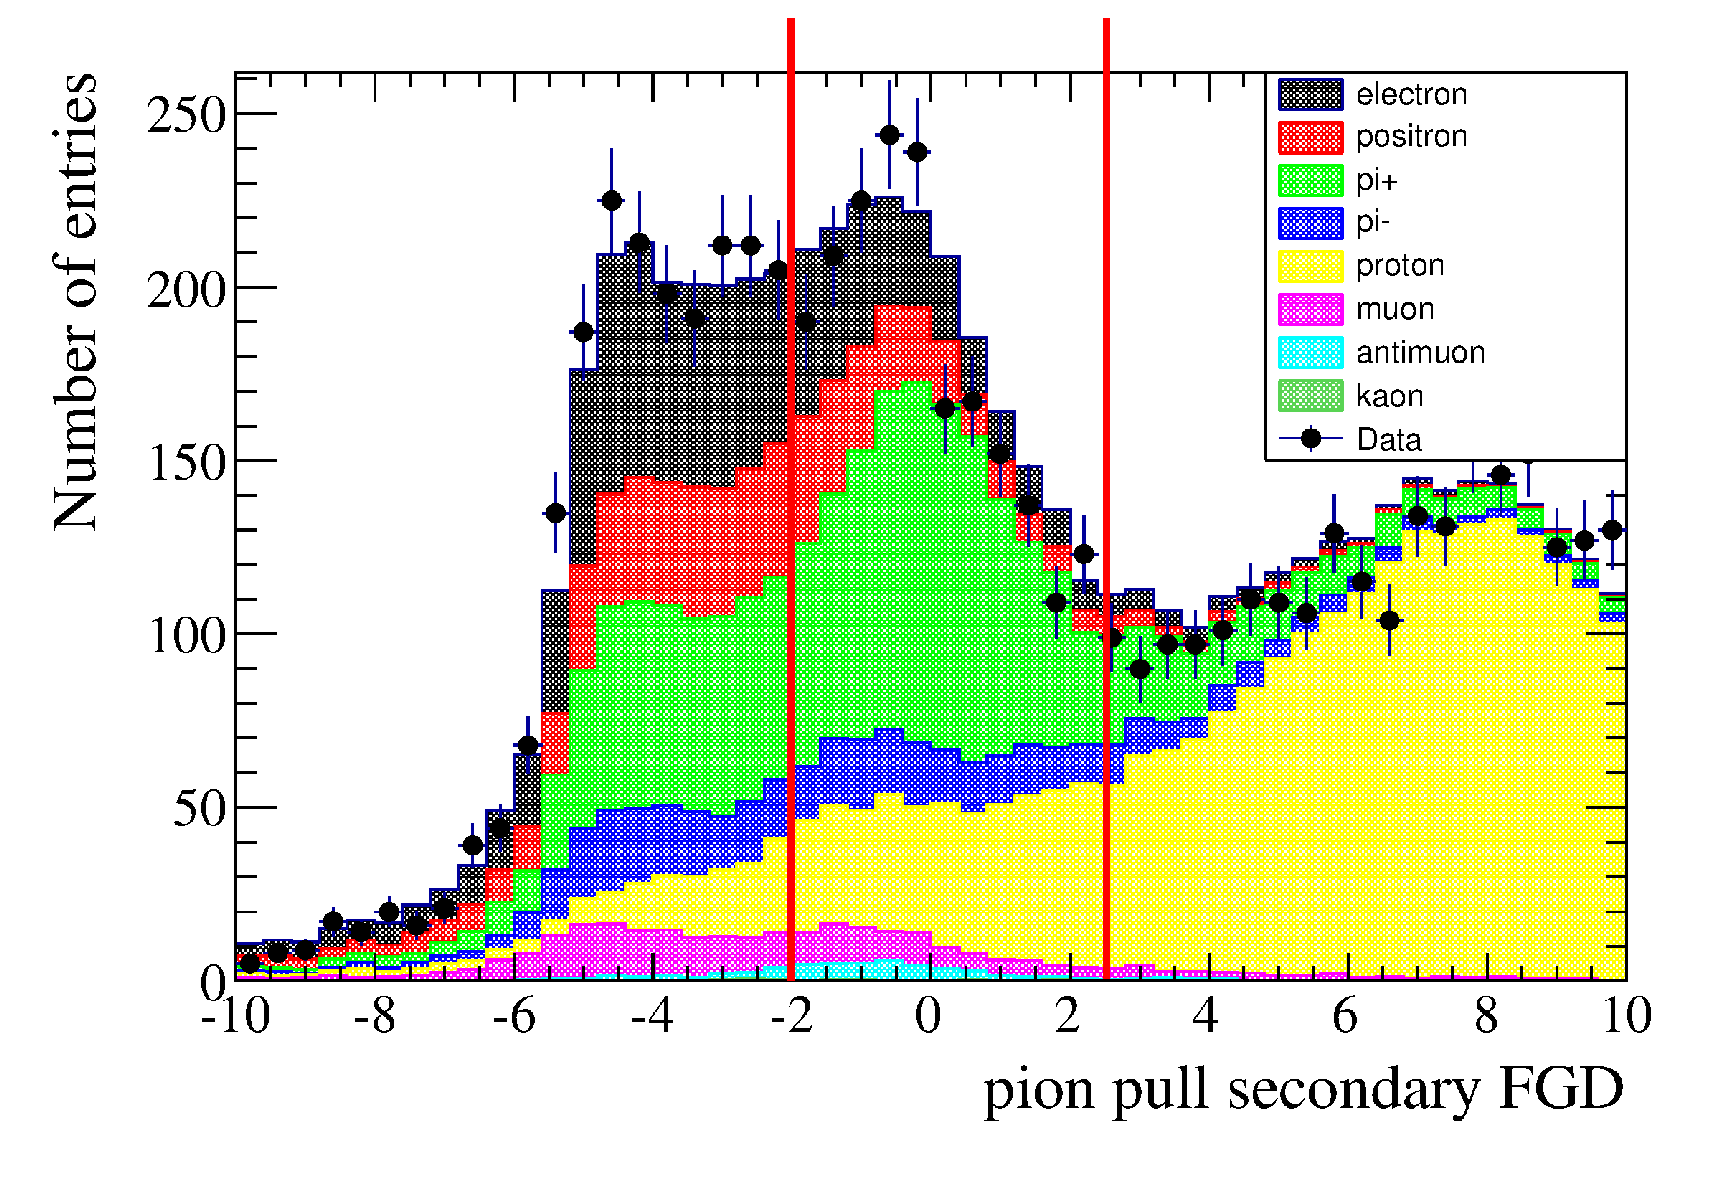
\includegraphics[width=0.5\textwidth]{figures/numu/Cuts/pull_secondarytrack_FGD_all.eps}
	\caption{FGD1 pion pulls for a fully contained track}
	\label{fig:FGD_pion_pulls}
\end{figure}

Then finally the remaining particles can be identified using the TPC PID: 
\begin{itemize}
	\item For a positive particle, it is tagged with type of highest probability. If the most likely particle is a positron but the $p_{reco} > 900\text{ MeV}$ it's tagged as a proton, otherwise a positron
	
	\item For a negative particle, if the probability of a pion is $P_\pi>0.8$ it is tagged as a negative pion, and if not it is assumed an electron
\end{itemize}

Now using information from the TPC PID, FGD Michel electron and FGD PID algorithms the \numu CC-inclusive sample can be categorised into the CC$0\pi$, CC$1\pi$ and CCOther samples:
\begin{itemize}
	\item \textbf{CC0$\pi$}: Contains events with no identified pions, electrons or positrons using the TPC PID. There are no Michel electrons and/or charged pions found in the FGD
	\item \textbf{CC$1\pi$}: Contains events with one reconstructed positively charged pion. The sum of the number of positive pions found in the TPC and the number of Michel electrons is one. If there are no Michel electrons the sum of positive pions in the TPC and fully contained in the FGD is one. If there is a negative pion or electron/positron reconstructed in the TPC it is rejected.
	\item \textbf{CCOther}: All events which are not classified as CC0$\pi$ or CC$1\pi$ fall into this sample. Events with one or more reconstructed negative pions, or neutral pions reconstructed as electron or positron candidates, in the TPC are thereby selected. Event with more than one positive pion based on the TPC and FGD pion counting criteria will also enter into this sample.
\end{itemize}

\paragraph{Efficiency and purity}
Using the aforementioned cuts we can study the lepton tagging efficiency and purity of each ND280 \numu selection. The number of events are the raw number of generated Monte-Carlo events without any weighting applied. We show the efficiencies as a function of reconstructed lepton candidate momentum, $p_{reco}$.

\autoref{fig:cc0pi_topology} shows the topology purity for the CC0$\pi$ selection in FGD1 and FGD2. The purity peak coincides with the event peak with $\sim85\%$ efficiency and falls off in both directions. The true CC$1\pi$ and CCOther topology constitute the selection very similarly, at about $10\%$ across the momentum range. As we move up in momentum the CC DIS cross-sections---the largest contribution to the CCOther final state---increase whilst the CCQE and 2p2h cross-sections---the largest contributions to the CC0$\pi$ final state---decrease. CC1$\pi$ and CC DIS interactions can produce low-momentum pions which aren't reconstructed in the detector and CC DIS can produce a $\pi^-$ which may be mistaken for the lepton candidate \red{show plots of cross-sections?}. Furthermore, the pions can undergo secondary interactions after exiting the nucleus, causing them to be undetected. The NC contribution comes primarily from the NC$1\pi^-$ via resonance interaction, in which the $\pi^-$ is identified as the lepton candidate and there are no other particles in the final state. We also note barely any anti-neutrino contamination, owing to the sign selection from the magnet, the low \numubar flux in FHC and the smaller cross-section. Averaging over the entire range we have purity of $75.5\%$ for FGD1 and $73.5\%$ for FGD2.
\begin{figure}[h]
	\begin{subfigure}[t]{0.49\textwidth}
		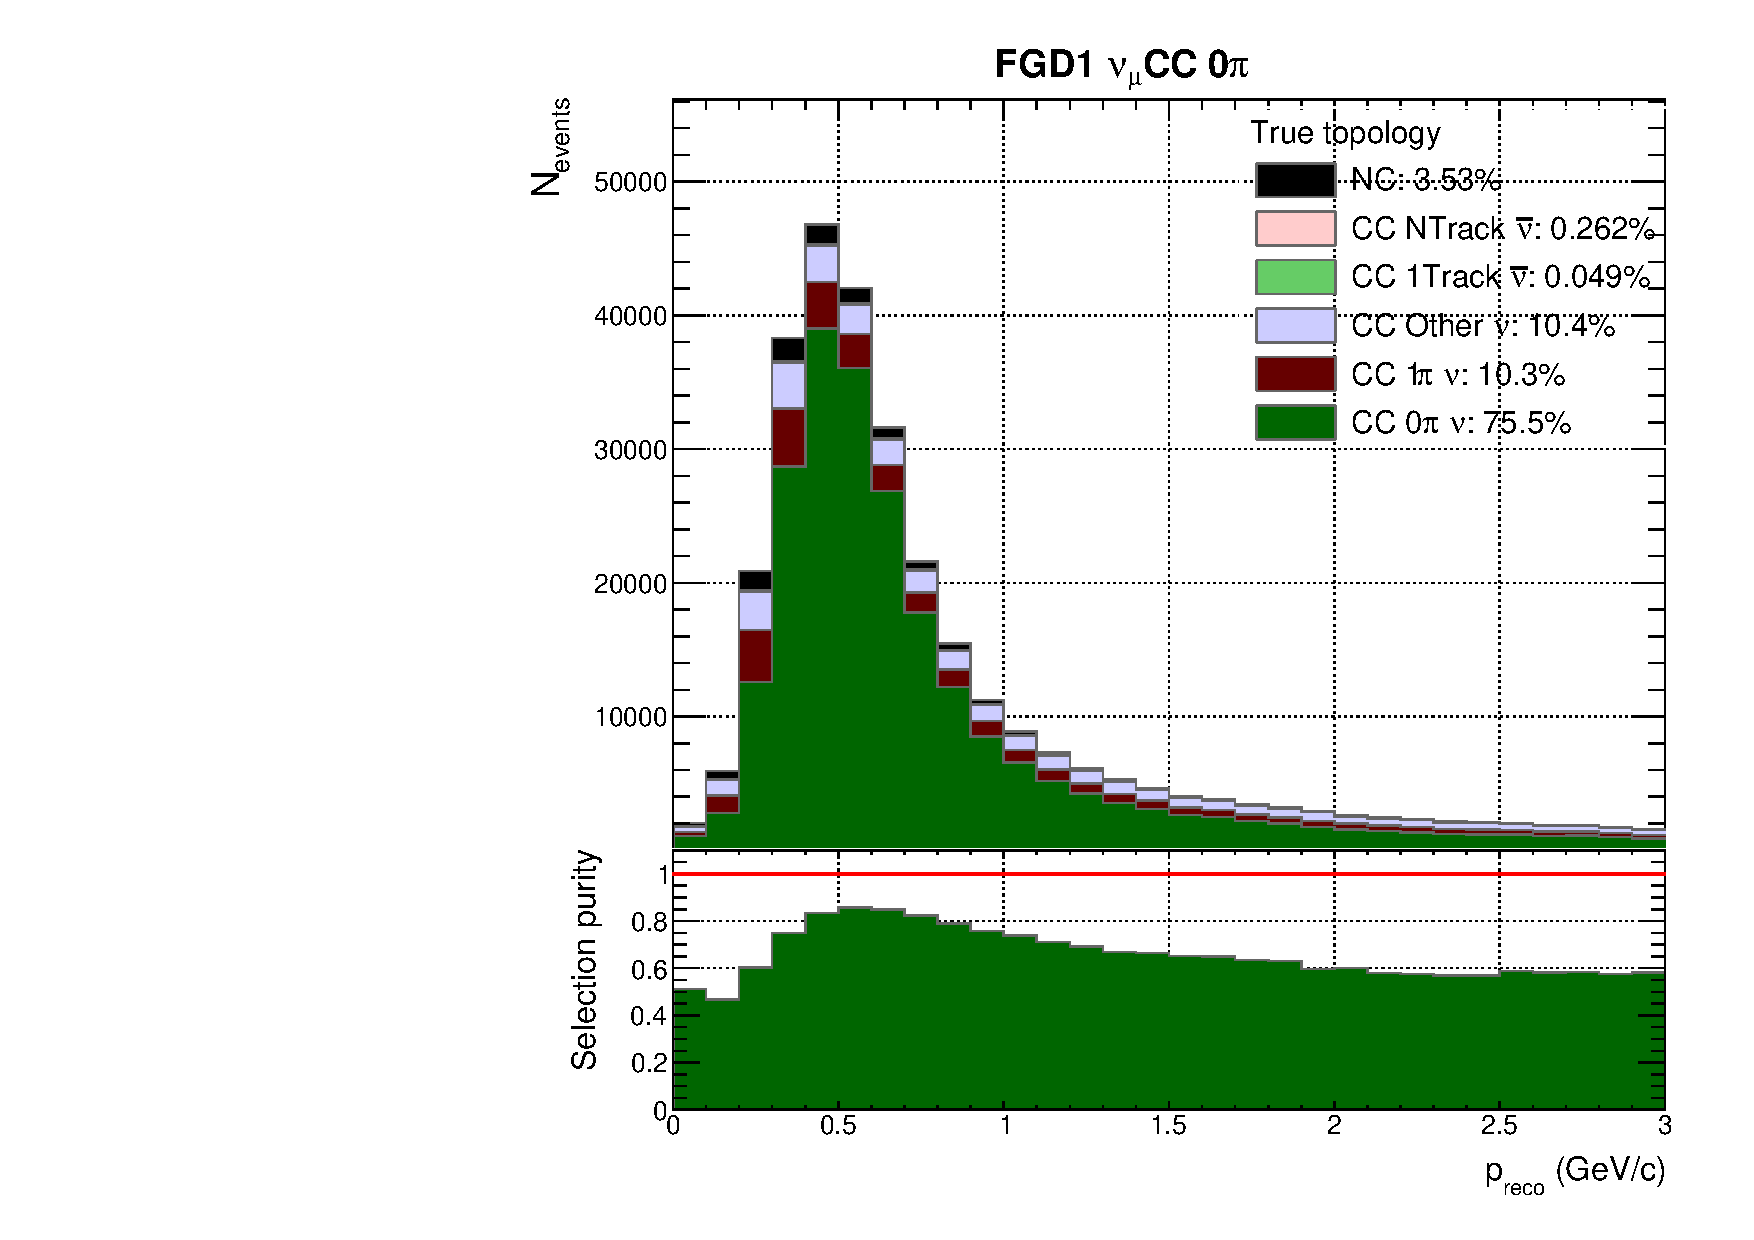
\includegraphics[width=\textwidth,page=1, trim={0mm 0mm 0mm 9mm}, clip]{figures/mach3/selection/2017b_Diag_WithSelection}
		\caption{FGD1}
	\end{subfigure}
	\begin{subfigure}[t]{0.49\textwidth}
		\includegraphics[width=\textwidth,page=7, trim={0mm 0mm 0mm 9mm}, clip]{figures/mach3/selection/2017b_Diag_WithSelection}
		\caption{FGD2}
	\end{subfigure}
	\caption{Breakdown of CC0$\pi$ selection events' true event topology for FGD1 and FGD2 }
	\label{fig:cc0pi_topology}
\end{figure}

\autoref{fig:cc0pi_muon} shows the muon tagging efficiency. We observe good performance over the range of muon momentum, starting with $\sim65\%$ at low momentum, plateauing at $\sim95\%$ above 500 MeV/c for both FGD1 and FGD2, which is where the majority of events reside. Averaging over the entire range, the muon tagging performance is 93.8\% for FGD1 and 93.2\% for FGD2. The largest background is $\pi^-$ from CC$1\pi$, CCOther and NC interactions, in which the $\pi^-$ is either created at the interaction vertex---e.g. an NC$1\pi^-$ via a resonance where there is no $\mu^-$, or a CCOther interaction creating multiple pions in which one $\pi^-$ has a higher reconstructed momentum than the $\mu^-$---or through final-state-interactions (FSI) in which a nucleon, $\pi^0$ or $\pi^+$ undergoes scattering on nucleons in the nucleus to produce the $\pi^-$.
\begin{figure}[!h]
	\begin{subfigure}[t]{0.49\textwidth}
		\includegraphics[width=\textwidth,page=2, trim={0mm 0mm 0mm 9mm}, clip]{figures/mach3/selection/2017b_Diag_WithSelection}
		\caption{FGD1}
	\end{subfigure}
	\begin{subfigure}[t]{0.49\textwidth}
		\includegraphics[width=\textwidth,page=8, trim={0mm 0mm 0mm 9mm}, clip]{figures/mach3/selection/2017b_Diag_WithSelection}
		\caption{FGD2}
	\end{subfigure}
	\caption{Breakdown of selection CC0$\pi$ events' true lepton candidate for FGD1 and FGD2 }
	\label{fig:cc0pi_muon}
\end{figure}

\autoref{fig:cc1pi_topology} shows the topology purity for the CC1$\pi$ selection. Owing to identifying one single $\pi^+$ and one single $\pi^-$, the purity is notably worse for CC1$\pi$ compared to CC0$\pi$ and peaks at $p_{reco}\sim0.4\text{ GeV/c}$ with $\sim70\%$ purity. The purity takes the biggest hit from CCOther feed-down at $25\%$, in which either the lepton candidate is identified as a $\pi^-$ with an accompanying $\pi^+$, or events with a \{$\mu^-$, $\pi^+$, $\pi^{-,0}$\} have the latter pion unreconstructed from high-angle and low momentum tracks, leading to a poorly determined PID. The CCOther feed-down increases with $p_{reco}$ as the CC DIS cross-section increases: the main cause of the decreasing purity with increase $p_{reco}$. The CC0$\pi$ contributions comes from the outgoing proton being reconstructed as a $\pi^+$, or when the nucleon rescatters after exiting the nucleus, producing a pion-like track that gets associated with the primary vertex by mistake. The CC0$\pi$ contribution is concentrated in the first momentum bin, in which it makes up $\sim50\%$. The NC topology contributes 7\% by producing a \{$\pi^-$, $\pi^+$\} state through NC DIS or NC1$\pi$ with FSI which gets reconstructed as the \{$\mu^-$, $\pi^+$\} final state. The purity for CC1$\pi$ across the full momentum range is $58\%$ and very similar for FGD1 and FGD2.
\begin{figure}[!h]
	\begin{subfigure}[t]{0.49\textwidth}
		\includegraphics[width=\textwidth,page=3, trim={0mm 0mm 0mm 9mm}, clip]{figures/mach3/selection/2017b_Diag_WithSelection}
		\caption{FGD1}
	\end{subfigure}
	\begin{subfigure}[t]{0.49\textwidth}
		\includegraphics[width=\textwidth,page=9, trim={0mm 0mm 0mm 9mm}, clip]{figures/mach3/selection/2017b_Diag_WithSelection}
		\caption{FGD2}
	\end{subfigure}
	\caption{Breakdown of selection CC1$\pi$ events' true event topology for FGD1 and FGD2 }
	\label{fig:cc1pi_topology}
\end{figure}

\autoref{fig:cc1pi_muon} shows the muon tagging efficiency for CC1$\pi^+$. As for the purity, the efficiency is comparably worse due to the additional pion requirement, averaging at 83\% across the $p_{reco}$ range. Common with the CC0$\pi$ efficiency in \autoref{fig:cc0pi_muon} the major background is $\pi^-$, which now constitutes 11\% instead of 4\%. The $\pi^-$ comes primarily from DIS interactions and CC1$\pi^0$ via resonances in which the $\pi^0$ undergoes a charge-exchange FSI, as discussed earlier. The $\pi^+$ contribution comes from high momentum pions which do not bend sufficiently to get a good PID: since the initial CC-inclusive search is done based on highest-momentum track this track is selected as the lepton candidate which curves similarly to a high-momentum $\mu^-$. As $p_{reco}$ increases the efficiency tends to similar values as the CC0$\pi$ selection.
\begin{figure}[!h]
	\begin{subfigure}[t]{0.49\textwidth}
		\includegraphics[width=\textwidth,page=4, trim={0mm 0mm 0mm 9mm}, clip]{figures/mach3/selection/2017b_Diag_WithSelection}
		\caption{FGD1}
	\end{subfigure}
	\begin{subfigure}[t]{0.49\textwidth}
		\includegraphics[width=\textwidth,page=10, trim={0mm 0mm 0mm 9mm}, clip]{figures/mach3/selection/2017b_Diag_WithSelection}
		\caption{FGD2}
	\end{subfigure}
	\caption{Breakdown of selection CC1$\pi$ events' true lepton candidate for FGD1 and FGD2 }
	\label{fig:cc1pi_muon}
\end{figure}

\red{Add part looking at how the pion is tagged and number of events}

\red{Show plots for \cosmu?}

\autoref{fig:ccoth_topology} shows the topology purity for the CCOther selection. As expected from the other purities, CCOther increases with $p_{reco}$ due to the increase in the CC DIS cross-section. The CC0$\pi$ and CC1$\pi$ topology seeps in to this selection by creating $\pi^{\pm,0}$ after exiting the nucleus that become(s) wrongly associated with the primary interaction vertex, or by the reconstruction falsely identifying an outgoing proton as a $\pi^+$. In the NC case, it is enough to have a interaction which produces a \{$\pi^-, \pi^0$\} combination, which can happen directly through NC DIS or indirectly with NC$1\pi$ via resonances, in which a secondary interaction occurs and the new track gets wrongly associated to the primary vertex. Initially, the purity starts at 35-40\% and plateaus around 80\% at $p_{reco} \sim 1.5\text{ GeV/c}$. Overall, the purity of the selection is 65\% for both FGDs over the entire range, with $\sim10\%$ each from NC, CC0$\pi$ and CC1$\pi$.
\begin{figure}[!h]
	\begin{subfigure}[t]{0.49\textwidth}
		\includegraphics[width=\textwidth,page=5, trim={0mm 0mm 0mm 9mm}, clip]{figures/mach3/selection/2017b_Diag_WithSelection}
		\caption{FGD1}
	\end{subfigure}
	\begin{subfigure}[t]{0.49\textwidth}
		\includegraphics[width=\textwidth,page=11, trim={0mm 0mm 0mm 9mm}, clip]{figures/mach3/selection/2017b_Diag_WithSelection}
		\caption{FGD2}
	\end{subfigure}
	\caption{Breakdown of selection CCOther events' true event topology for FGD1 and FGD2 }
	\label{fig:ccoth_topology}
\end{figure}

\autoref{fig:ccoth_muon} shows the muon tag efficiency for the CC Other sample, which is notably worse than for previous selections: on average 73\%. This is expected, since the CCOther selection has at least 2 tracks (1$\mu^-$, 1$\pi^{\pm}$, 1$\pi^0$) but often even more. It is sufficient to have an interaction in which $N_\pi \ge 2$ and $p_{\pi} > p_{\mu}$ to wrongly identify the lepton candidate. Owing to the many tracks in this topology due to the CC and NC DIS interaction, it is no surprise to see a 20\% contribution from $\pi^-$. Furthermore, at low $p_{reco}$ electrons are selected a majority of the time, coming from two sources: 1) relatively high threshold of \numu CC DIS compared to \nue CC DIS due to the muon mass (even though the \nue flux is much lower than \numu \red{show this}) and 2) since the CCOther topology is the only topology to allow for $\pi^0$, these are likely to produce $e^\pm$ pairs in the TPC. If the $\pi^0$ shower occurs early in the TPC and the interaction vertex is traced to a downstream layer of the FGD, the electron may be falsely associated with the interaction vertex, and if $p_e > p_\mu$ is picked as the highest momentum candidate. To pass the TPC $\mu$ PID cut we would require a low momentum $e^-$ to match the dE/dx of a $\mu^-$, which in \autoref{fig:TPC_dedx} happens at $p\sim100\text{ MeV/c}$.
\begin{figure}[h]
	\begin{subfigure}[t]{0.49\textwidth}
		\includegraphics[width=\textwidth,page=6, trim={0mm 0mm 0mm 9mm}, clip]{figures/mach3/selection/2017b_Diag_WithSelection}
		\caption{FGD1}
	\end{subfigure}
	\begin{subfigure}[t]{0.49\textwidth}
		\includegraphics[width=\textwidth,page=12, trim={0mm 0mm 0mm 9mm}, clip]{figures/mach3/selection/2017b_Diag_WithSelection}
		\caption{FGD2}
	\end{subfigure}
	\caption{Breakdown of selection CCOther events' true lepton candidate for FGD1 and FGD2 }
	\label{fig:ccoth_muon}
\end{figure}

\subsection{Event selection cuts, \numubar in RHC}
\label{sec:numubar_sel}
The anti-neutrino selections CC1Track and CCNTrack have the same event quality and fiducial volume cut as the neutrino selection, and the muon candidate track is required to pass through the TPC downstream of the struck FGD. However, its highest momentum track is required to be the highest momentum positive track for its muon PID (a $\mu^+$ coming from a \numubar interaction). Furthermore, it has a larger background of ``wrong-sign'' events: \numu interactions producing $\mu^-$, but also \numu interactions producing $\pi^+$ which may be identified as the lepton candidate.\red{SHOW PLOT OF THIS, e.g. numubar flux with numu background in there} Hence, the selection cuts proceed marginally differently:
\begin{itemize}
	\item \textbf{Positive multiplicity}: The muon candidate track charge is required to be a highest momentum positive track, which removes a large amount of \numu background interactions
	
	\item \textbf{TPC veto}: Veto backwards-going events starting in the FGD and events coming from the P0D and the magnet by utilising the upstream TPCs. If the upstream TPC of an FGD has hits the event is rejected
	
	\item \textbf{Positive muon identification}: The TPC PID outlined for the \numu selections are used to select the positive muon candidate, with the cuts optimised for $\mu^+$. 
	
	$\mathcal{L}_{MIP}$ is defined identically to \autoref{eq:tpc_track_mip} although the cut is now placed at 0.9, and still applies only to particles with $p < 500\text{ MeV}$. The muon likelihood $\mathcal{L}_\mu$ is also modified to $0.1 < \mathcal{L}_\mu < 0.7$ which removes protons and positive pions from the \numu background. The upper bound at 0.7 is present to reject low energy wrong-sign muons ($\mu^-$), which are misidentified as positive tracks. The likelihood distributions and impact of these cuts are shown in \autoref{fig:numubar_likelihood} and \autoref{fig:numubar_likelihood_sel} for the selected lepton candidate. \autoref{fig:numubar_pulls} shows the TPC PID pulls for run5+6. \red{REMEMBER THAT THIS IS NOT PRESENT FOR PSYCHE V3}
\end{itemize}

\begin{figure}[!h]
	\begin{subfigure}[t]{0.49\textwidth}
		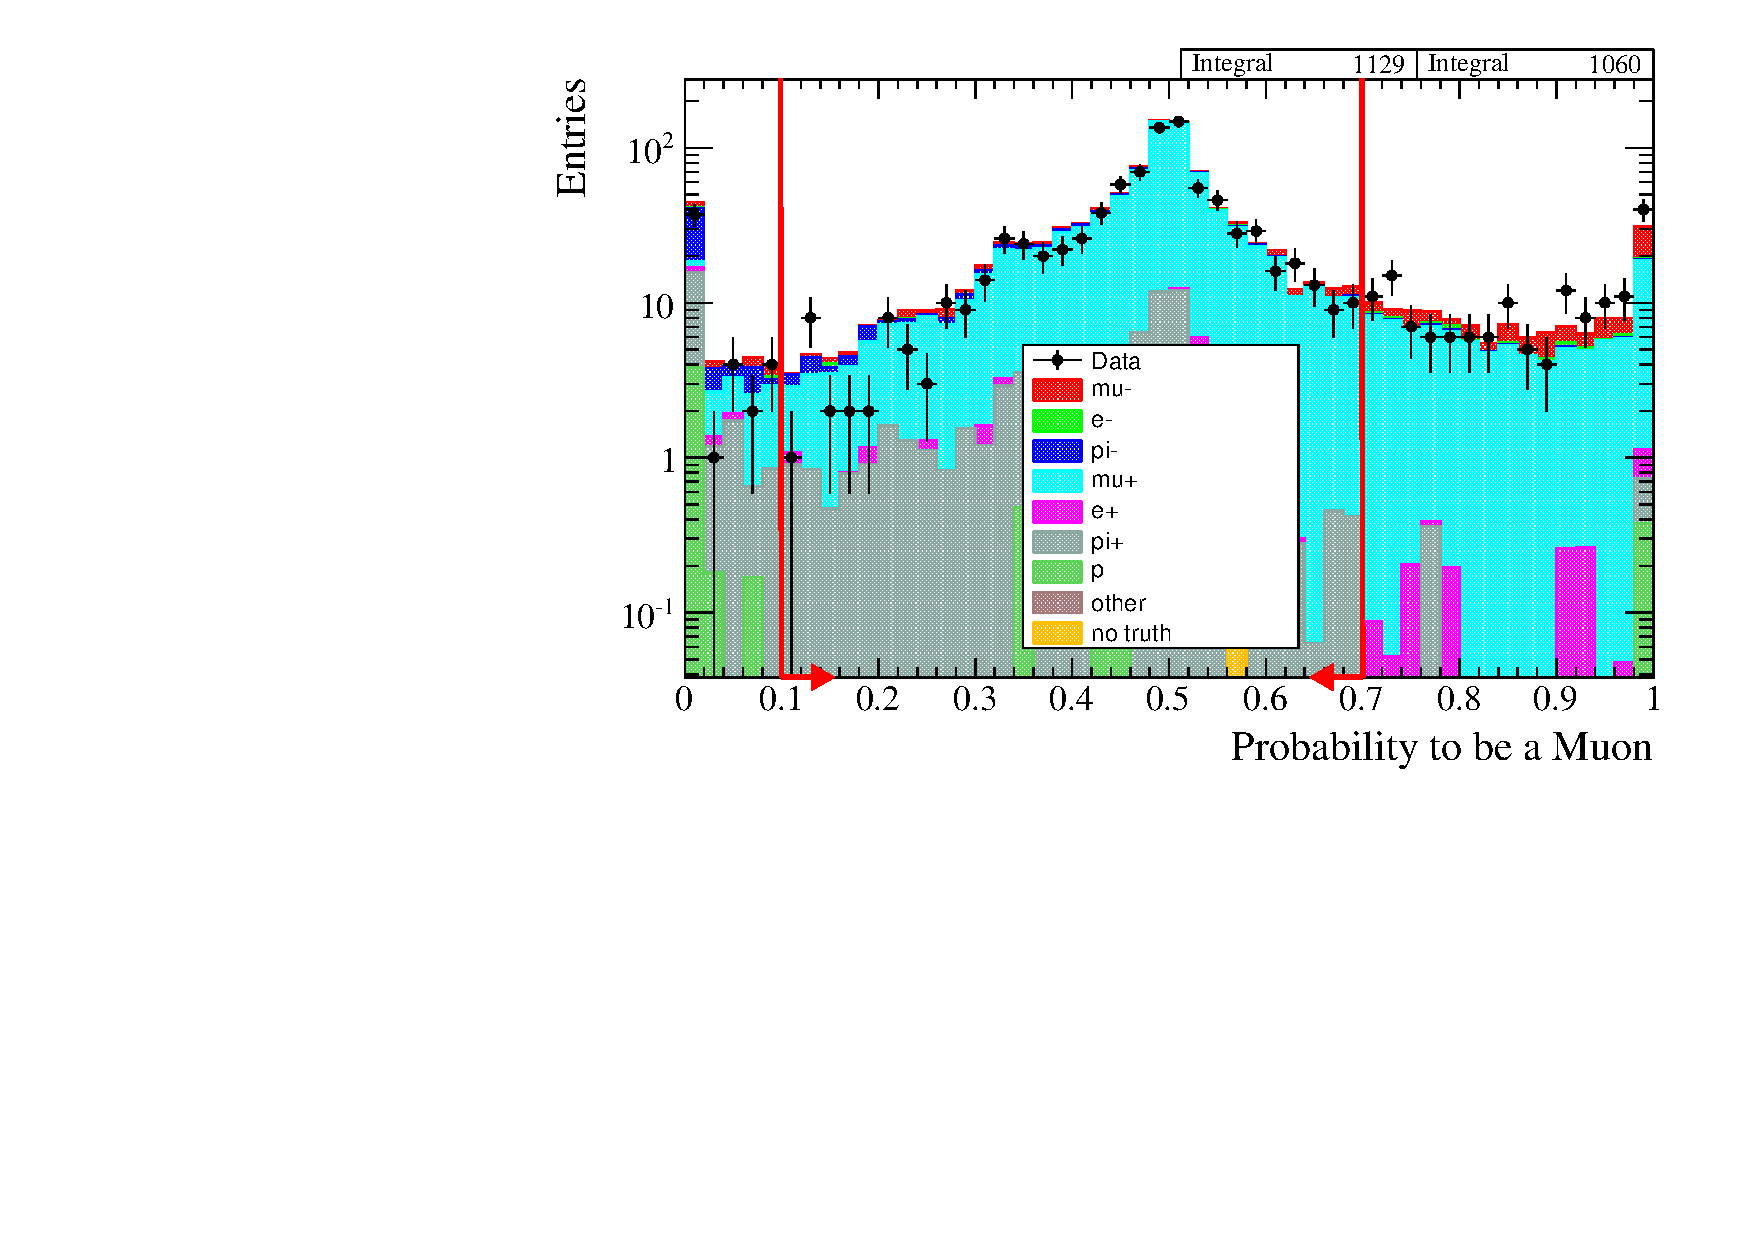
\includegraphics[width=\textwidth]{figures/numu/Cuts/numubar/likemu_numubar}
		\caption{$\mathcal{L}_\mu$}
	\end{subfigure}
	\begin{subfigure}[t]{0.49\textwidth}
		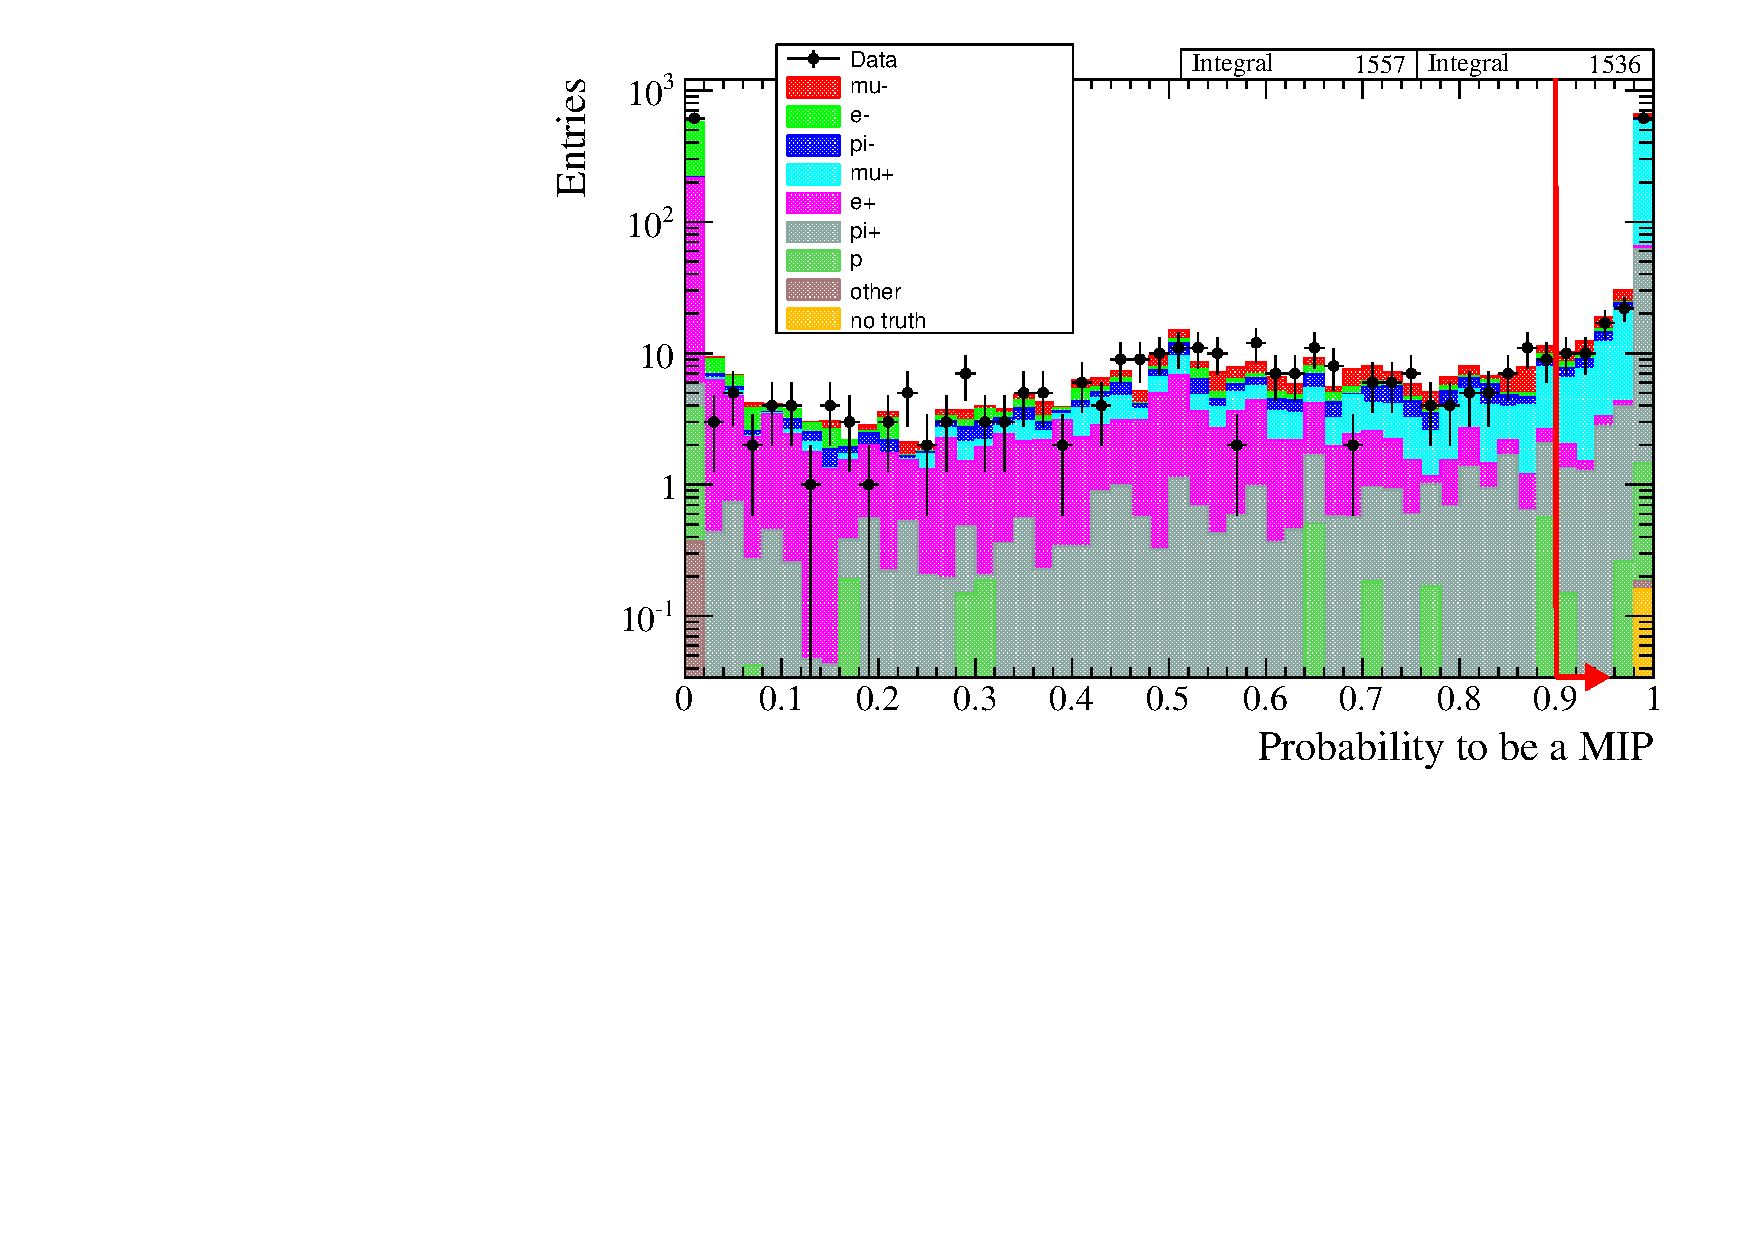
\includegraphics[width=\textwidth]{figures/numu/Cuts/numubar/likemip_numubar}
		\caption{$\mathcal{L}_{MIP}$}
	\end{subfigure}
	\caption{Likelihood distributions for $\mu$ and MIP using run5+6 \numubar data, used in \numubar RHC selections}
	\label{fig:numubar_likelihood}
\end{figure}

\begin{figure}[!h]
	\begin{subfigure}[t]{0.49\textwidth}
		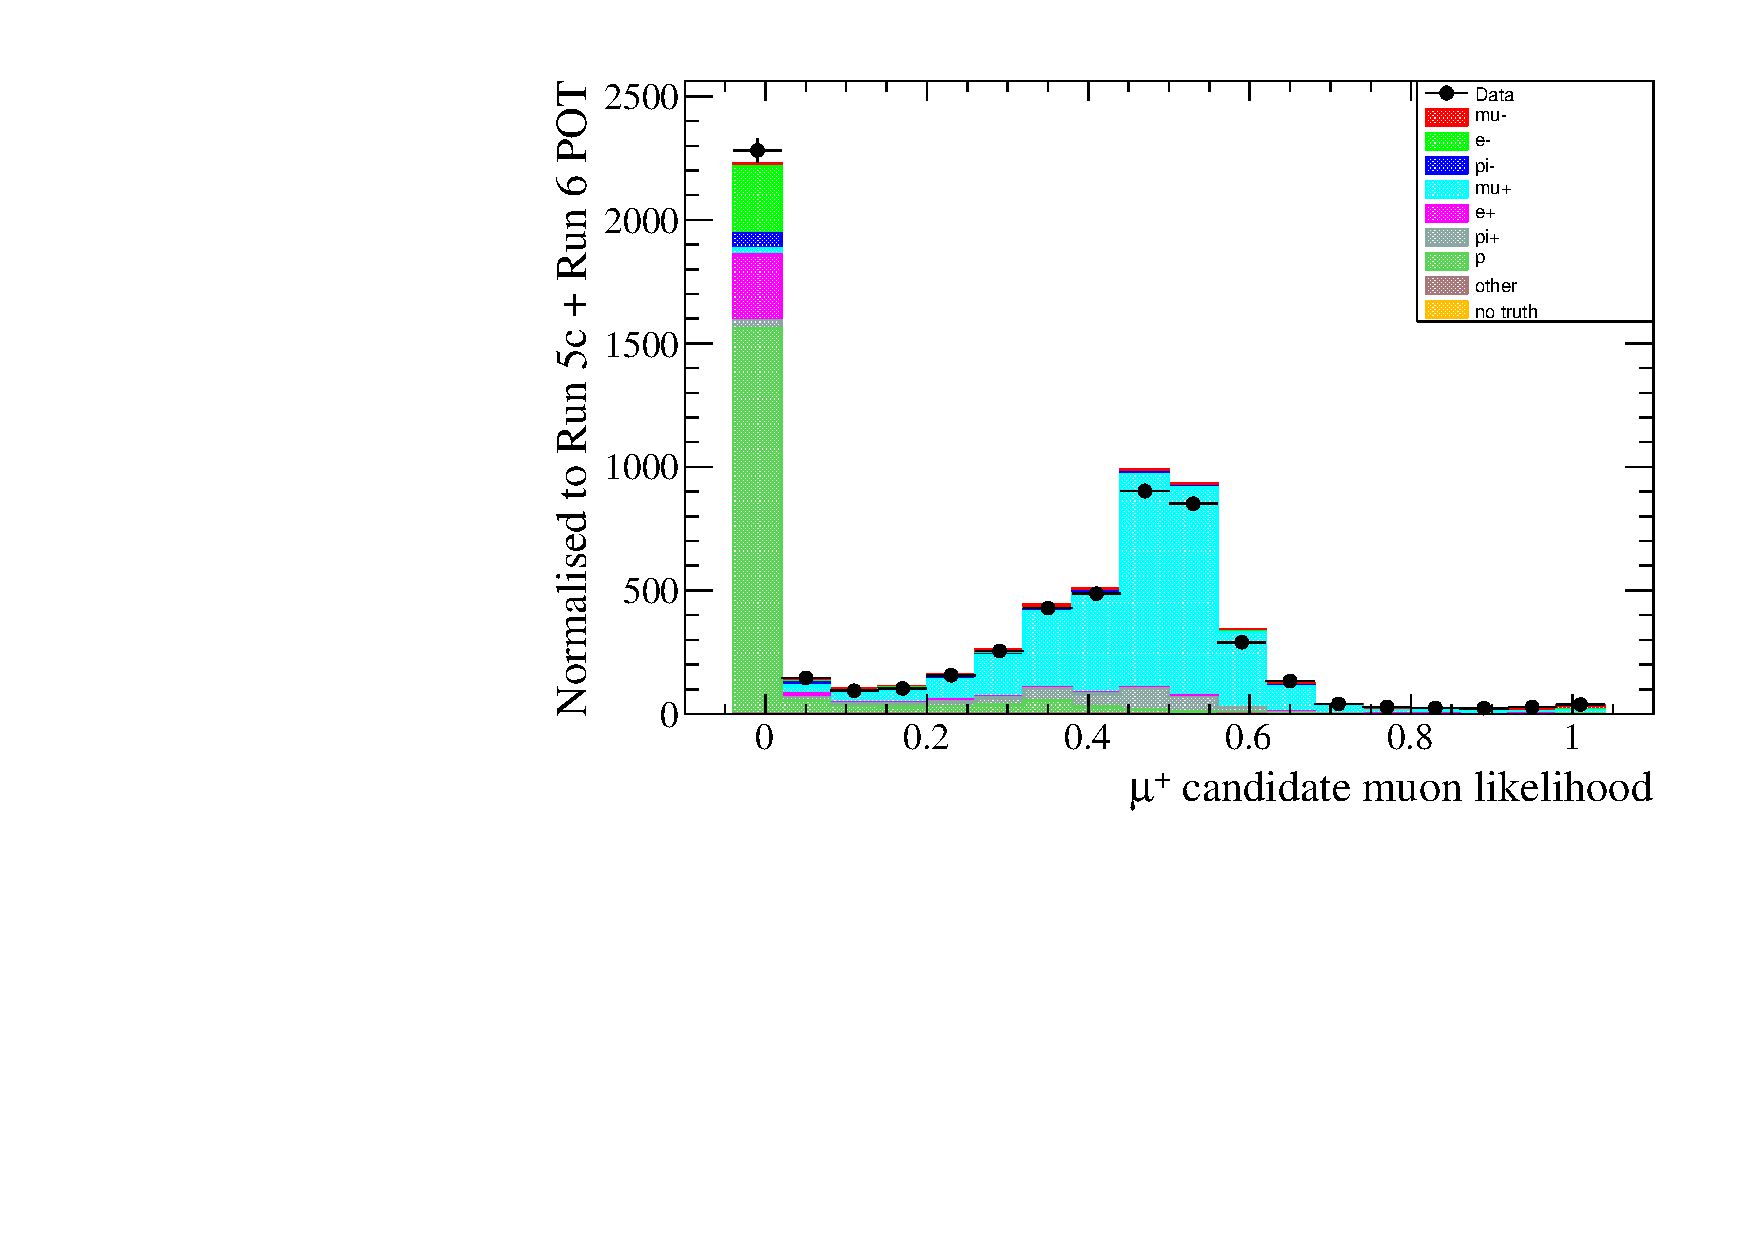
\includegraphics[width=\textwidth]{figures/numu/Cuts/numubar/selmu_likemu_particle}
		\caption{$\mathcal{L}_\mu$}
	\end{subfigure}
	\begin{subfigure}[t]{0.49\textwidth}
		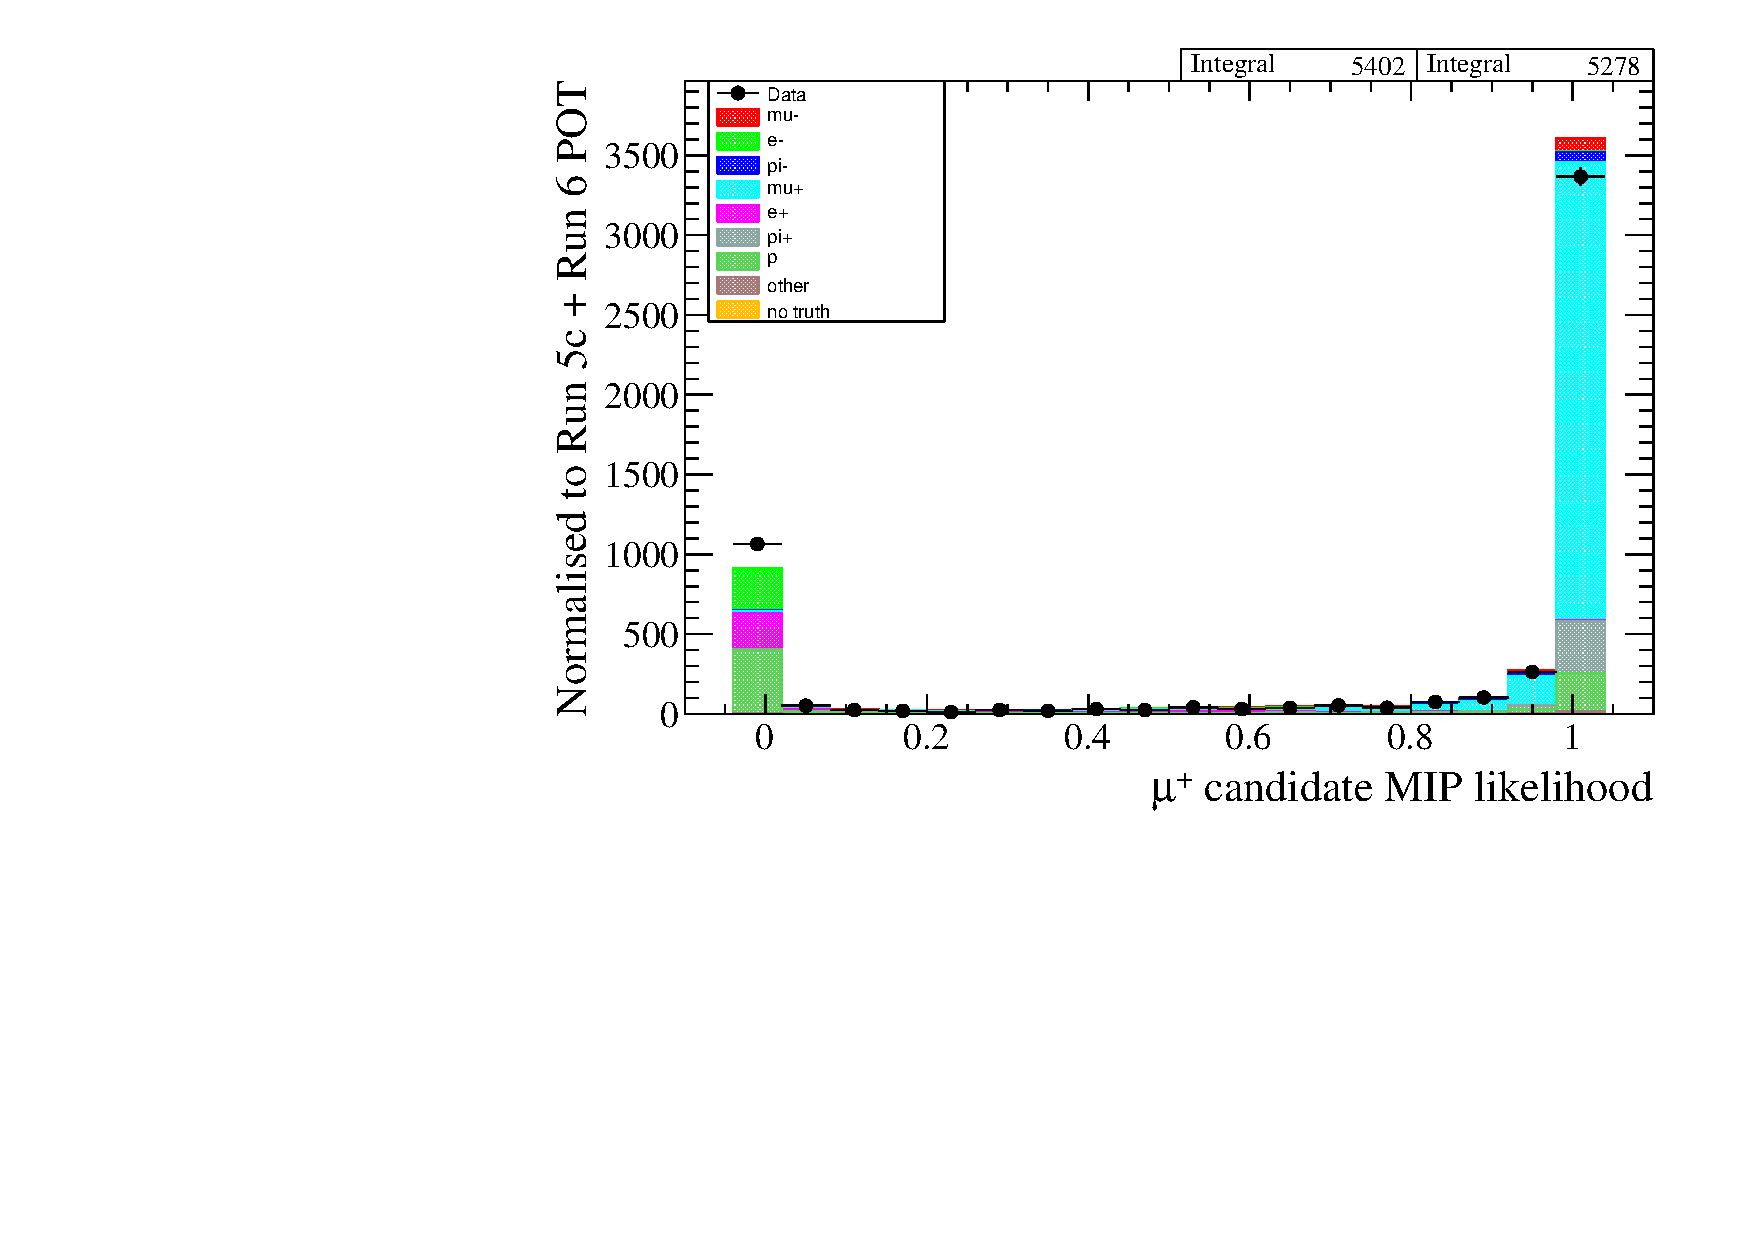
\includegraphics[width=\textwidth]{figures/numu/Cuts/numubar/selmu_likemip_particle}
		\caption{$\mathcal{L}_{MIP}$}
	\end{subfigure}
	\caption{Likelihood distributions for the selected lepton candidate using run5+6 \numubar data, used in \numubar RHC selections}
	\label{fig:numubar_likelihood_sel}
\end{figure}

\begin{figure}[!h]
	\begin{subfigure}[t]{0.32\textwidth}
		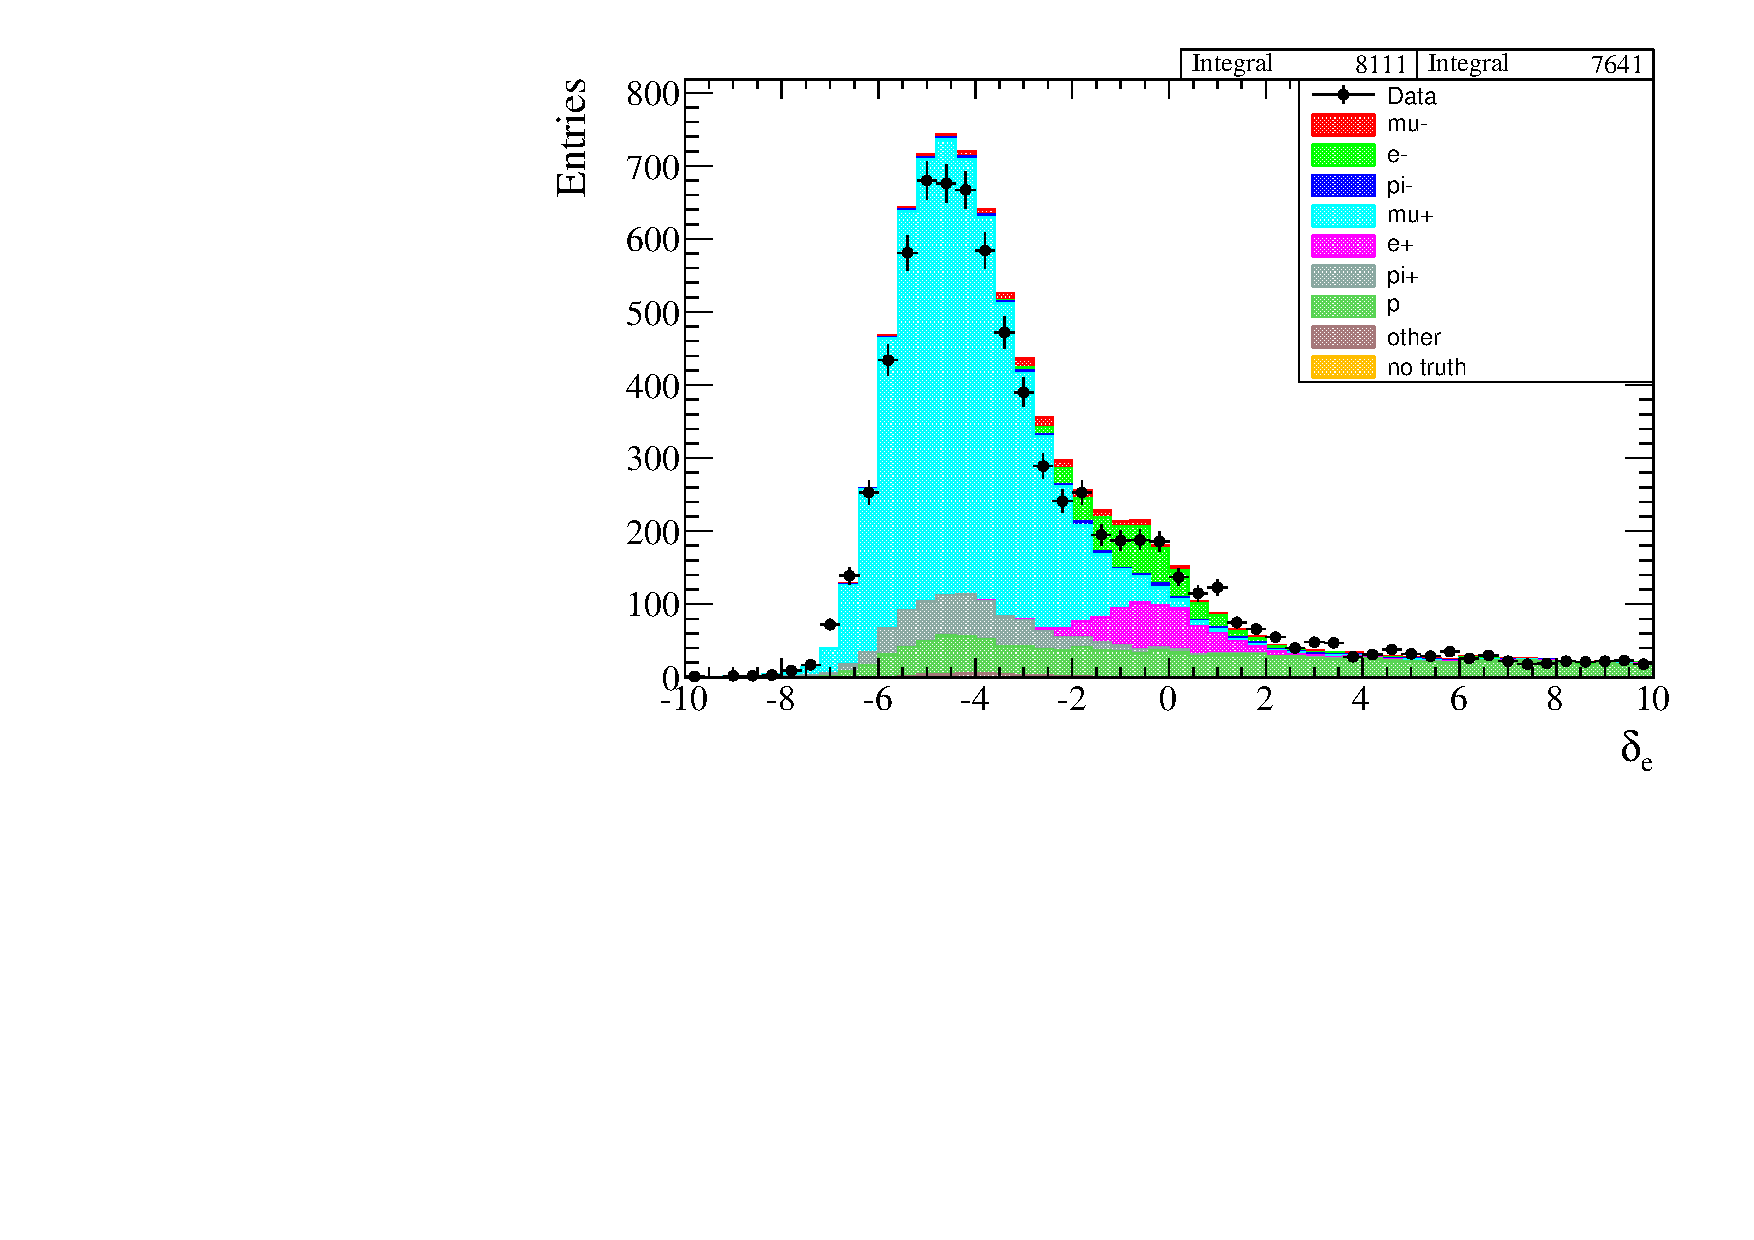
\includegraphics[width=\textwidth]{figures/numu/Cuts/numubar/presel_pullele_part}
		\caption{$Pull_e$}
	\end{subfigure}
	\begin{subfigure}[t]{0.32\textwidth}
		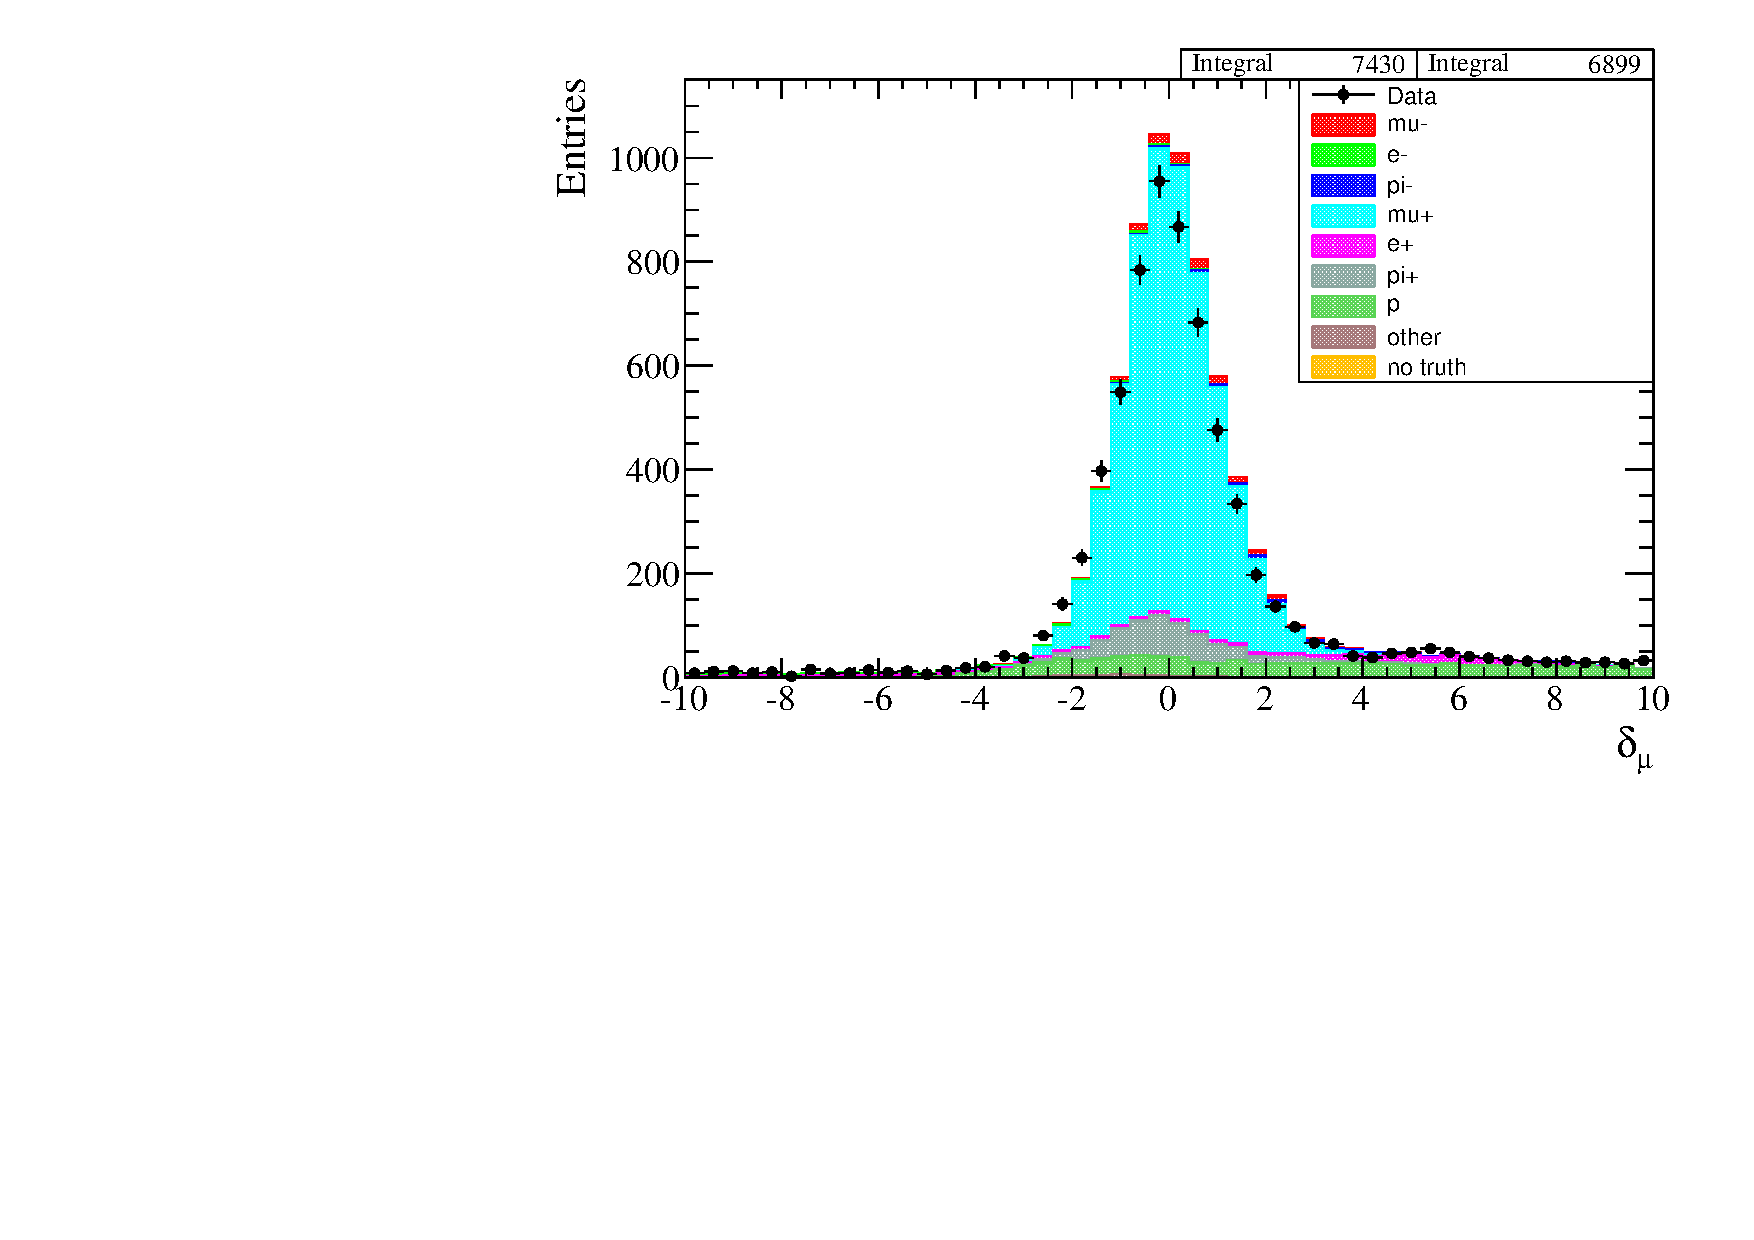
\includegraphics[width=\textwidth]{figures/numu/Cuts/numubar/presel_pullmu_part}
		\caption{$Pull_\mu$}
	\end{subfigure}
	\begin{subfigure}[t]{0.32\textwidth}
		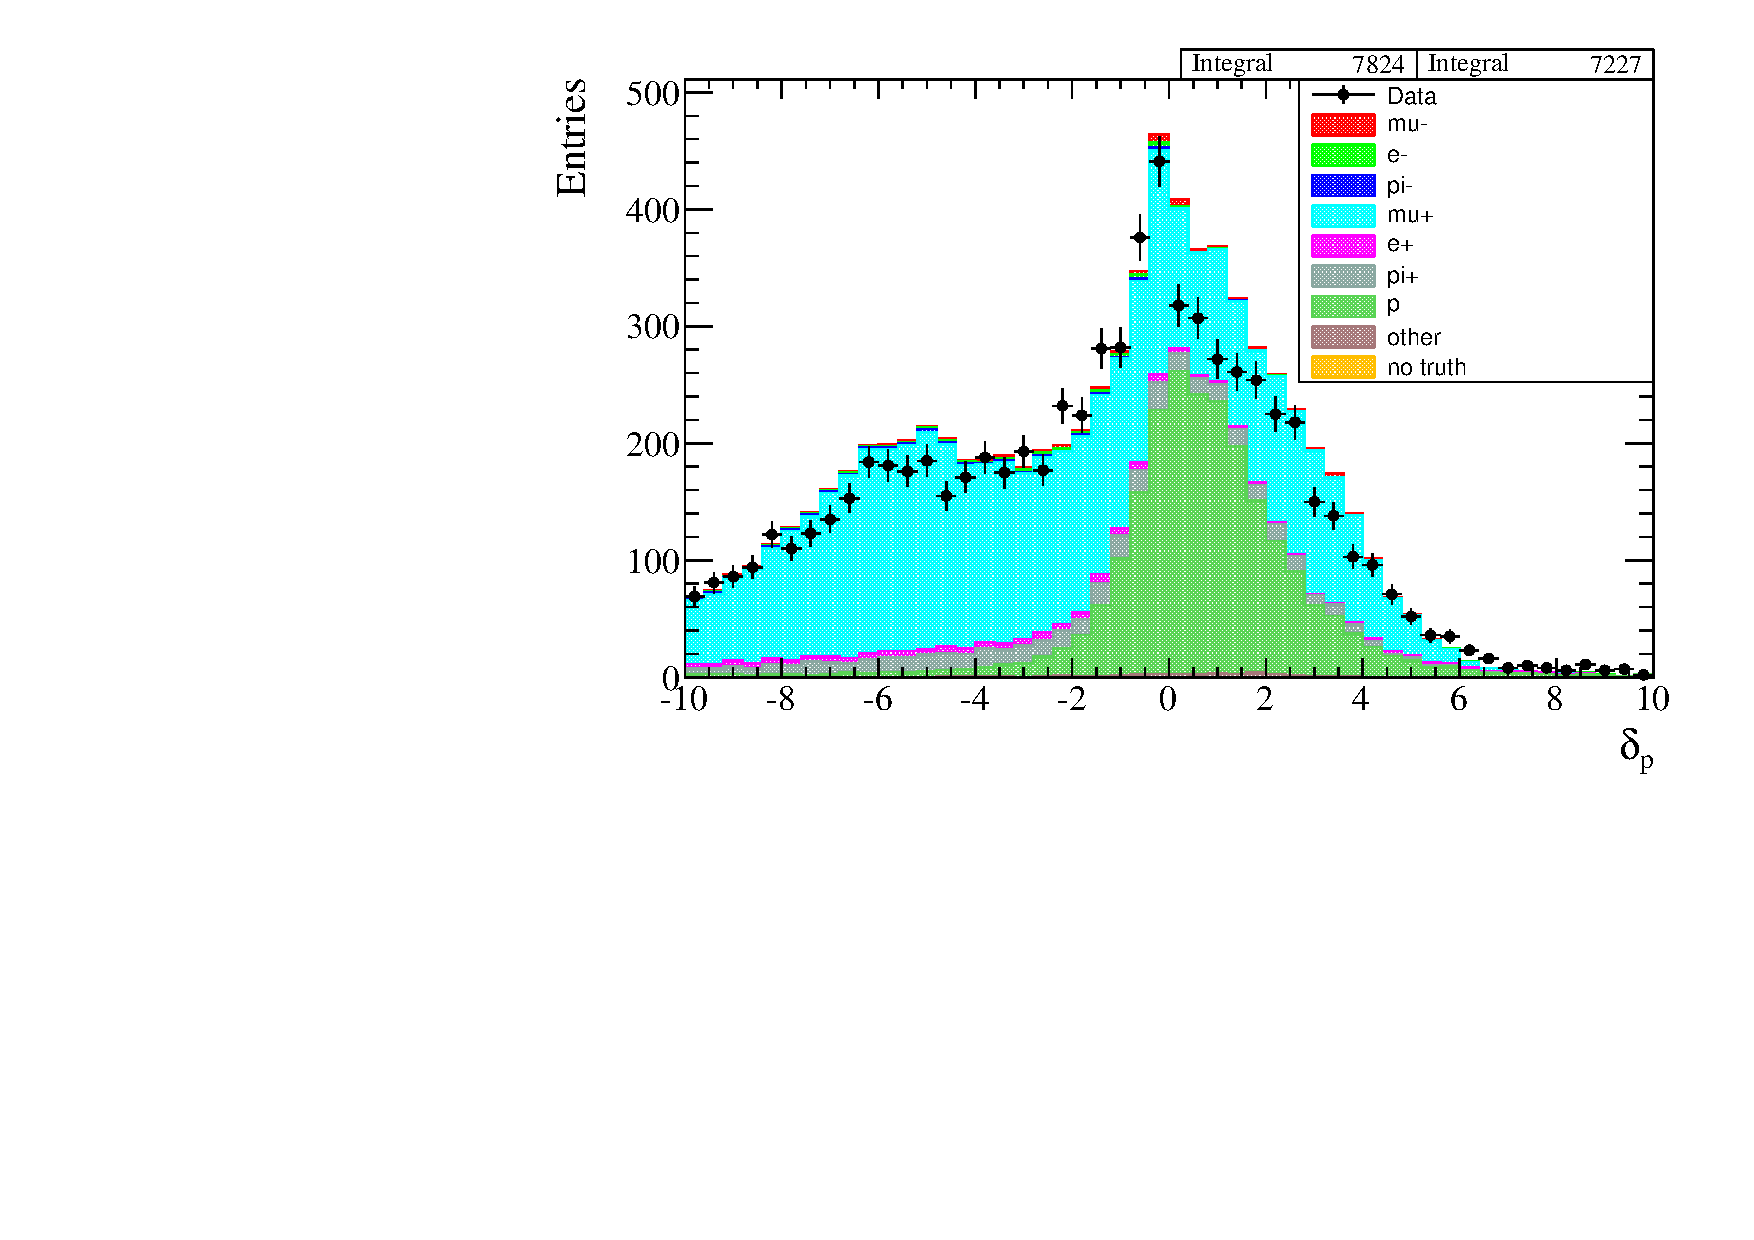
\includegraphics[width=\textwidth]{figures/numu/Cuts/numubar/presel_pullp_part}
		\caption{$Pull_p$}
	\end{subfigure}
	\caption{Pulls used in the TPC PID used in \numubar RHC selections}
	\label{fig:numubar_pulls}
\end{figure}

Once the \numubar CC-inclusive selection is run the aforementioned pion reconstruction is applied. The \numubar CC1Track selection has one positive muon and does not have any charged or neutral pions in the final state. Importantly, the \numubar CC1Track selection has a higher efficiency in selecting the muon candidate than the \numu CC0$\pi$ selection due to the \numubar resonant interactions producing a $\pi^-$, not a $\pi^+$, which are promptly absorbed in the nucleus and so do not leave a track to be (falsely) identified as a muon candidate. The \numubar CCNTrack selection contains the remaining particles passing the \numubar CC-inclusive selection, containing at least one neutral or charged pion and/or any number of heavier mesons.

\paragraph{Efficiency and purity}
As for the \numu case, we study the efficiency and purities of the anti-neutrino CC1Track and CCNTrack samples.

\autoref{fig:ccnubar1trk_topology} shows the \numubar CC 1 track topology purity. The purity peaks at 85\% with the event distribution peak ($p_{reco}\sim 0.6\text{ GeV}$) and decreases to $\sim60\%$ at higher momentum. The wrong-sign \numu equivalent selection have a small effect, notable only at low momentum. The largest background is the \numubar N tracks topology, in which one of the pions are unreconstructed. The NC topology enters primarily by the NC1$\pi^+$ via resonance interaction, in which the $\pi^+$ is reconstructed as a $\mu^+$. Over the whole range the purity is 76.7\% where the analogous \numu selection in \autoref{fig:cc0pi_topology} had a purity of 75.5\%, so are very similar in performance.
\begin{figure}[h]
	\begin{subfigure}[t]{0.49\textwidth}
		\includegraphics[width=\textwidth,page=13, trim={0mm 0mm 0mm 9mm}, clip]{figures/mach3/selection/2017b_Diag_WithSelection}
		\caption{FGD1}
	\end{subfigure}
	\begin{subfigure}[t]{0.49\textwidth}
		\includegraphics[width=\textwidth,page=17, trim={0mm 0mm 0mm 9mm}, clip]{figures/mach3/selection/2017b_Diag_WithSelection}
		\caption{FGD2}
	\end{subfigure}
	\caption{Breakdown of \numubar CC 1Trk selection events' true event topology for FGD1 and FGD2 }
	\label{fig:ccnubar1trk_topology}
\end{figure}

\autoref{fig:ccnubar1trk_muon} shows the muon efficiency for \numubar CC 1 track selection. As with the \numu selections, both FGDs have efficiencies of 90\% over the whole range, peaking at 95\% at the event distribution maximum around $p_{reco} \sim 0.5\text{ GeV/c}$. The wrong-sign (\numubar) background makes up 1\% of selected lepton candidates, and NC 5\%.
\begin{figure}[h]
	\begin{subfigure}[t]{0.49\textwidth}
		\includegraphics[width=\textwidth,page=14, trim={0mm 0mm 0mm 9mm}, clip]{figures/mach3/selection/2017b_Diag_WithSelection}
		\caption{FGD1}
	\end{subfigure}
	\begin{subfigure}[t]{0.49\textwidth}
		\includegraphics[width=\textwidth,page=18, trim={0mm 0mm 0mm 9mm}, clip]{figures/mach3/selection/2017b_Diag_WithSelection}
		\caption{FGD2}
	\end{subfigure}
	\caption{Breakdown of \numubar CC 1Trk selection events' true lepton candidate for FGD1 and FGD2 }
	\label{fig:ccnubar1trk_muon}
\end{figure}

As with the \numu samples, the CCNTrack selection purity in \autoref{fig:ccnubarNtrk_topology} is much lower than for the 1 track. It peaks at 60\% and decreases to 40\% at intermediate $p_{reco}$ to increase to 60\% at higher momentum. Overall, the wrong-sign CC N track topology (\numu) is the largest contribution at 27\%, the NC contribution is 14\% and \numubar CC 1 track is non-negligable at 12\% for both FGDs. Since the CCNtrack selection only requires $N>1$, the \numu CC N track enters by the \{$\mu^-$,$\pi^+$\} being identified as \{$\pi^-$, $\mu^+$\}, on top of the usual possibilities of broken tracks and missed secondary pions. The CC1Track contamination comes from energetic protons being reconstructed as a $\mu^+$ or $\pi^+$, and lesser so producing secondary pions and/or nucleons, leading to more particles associated with the primary vertex.
\begin{figure}[!h]
	\begin{subfigure}[t]{0.49\textwidth}
		\includegraphics[width=\textwidth,page=15, trim={0mm 0mm 0mm 9mm}, clip]{figures/mach3/selection/2017b_Diag_WithSelection}
		\caption{FGD1}
	\end{subfigure}
	\begin{subfigure}[t]{0.49\textwidth}
		\includegraphics[width=\textwidth,page=19, trim={0mm 0mm 0mm 9mm}, clip]{figures/mach3/selection/2017b_Diag_WithSelection}
		\caption{FGD2}
	\end{subfigure}
	\caption{Breakdown of \numubar CC NTrk selection events' true event topology for FGD1 and FGD2 }
	\label{fig:ccnubarNtrk_topology}
\end{figure}

\autoref{fig:ccnubarNtrk_muon} shows the selected lepton candidate, which over the entire momentum range is 54\%. At low momentum the efficiency is very poor but peaks at $p_{reco} \sim 0.5 \text{ GeV/c}$ at about 60\%. $\pi^+$ make up $\sim24\%$ of the lepton candidates, having the largest impact between 0.5-1.5 GeV/c. At $\sim 1.5\text{ GeV/c}$ the ``Other'' category rises sharply, making up 30\% of the lepton candidates. This population is predominantly protons being identified as $\mu^+$ in the TPC PID algorithm due to the dE/dx, which happens when $1.3 < p < 1.7 \text{ GeV/c}$ as seen in \autoref{fig:TPC_dedx}. Looking ahead at the \numu in RHC muon efficiency in \autoref{fig:ccnubarnuNtrk_muon}, the ``Other'' population contributes a mere 0.6\% over the entire momentum range since the lepton candidate is required to be of negative charge. After the proton ``bump'' the efficiency rises to 60\% again.
\begin{figure}[!h]
	\begin{subfigure}[t]{0.49\textwidth}
		\includegraphics[width=\textwidth,page=16, trim={0mm 0mm 0mm 9mm}, clip]{figures/mach3/selection/2017b_Diag_WithSelection}
		\caption{FGD1}
	\end{subfigure}
	\begin{subfigure}[t]{0.49\textwidth}
		\includegraphics[width=\textwidth,page=20, trim={0mm 0mm 0mm 9mm}, clip]{figures/mach3/selection/2017b_Diag_WithSelection}
		\caption{FGD2}
	\end{subfigure}
	\caption{Breakdown of \numubar CC NTrk selection events' true lepton candidate for FGD1 and FGD2 }
	\label{fig:ccnubarNtrk_muon}
\end{figure}

\subsection{Event selection, \numu in RHC}
\label{sec:numu_in_nubar_sel}
In anti-neutrino mode there is a large fraction of \numu interactions, owing partly to the larger \numu cross-section and partly due to the higher flux background. \red{show plots of this}. The same pre-selection cuts apply for the \numu in RHC selection as for the previous selections presented in \autoref{sec:numu_sel} and \autoref{sec:numubar_sel}.

The CC-inclusive selection proceeds by:
\begin{itemize}
	\item \textbf{Negative multiplicity}: The highest momentum track is required to be the highest momentum negative track, which starts the seeding track. The $\mu^-$ identification uses the TPC PID on the highest momentum negative track. 
	
	\item \textbf{TPC PID}: The PID proceeds by the MIP requirement in \autoref{eq:tpc_track_mip} for particles with $p_\mu < 500 \text{ MeV/c}$, accepting candidate tracks with $\mathcal{L}_{MIP} > 0.7$.
	
	Similar to \autoref{sec:numubar_sel}, a lower and upper bound is set $0.1 < \mathcal{L}_\mu < 0.8$, which rejects protons and mis-reconstructed $\mu^+$. The effect of these cuts can be seen in \autoref{fig:nu_numubar_likelihood}.
\end{itemize}

\begin{figure}[!h]
	\begin{subfigure}[t]{0.49\textwidth}
		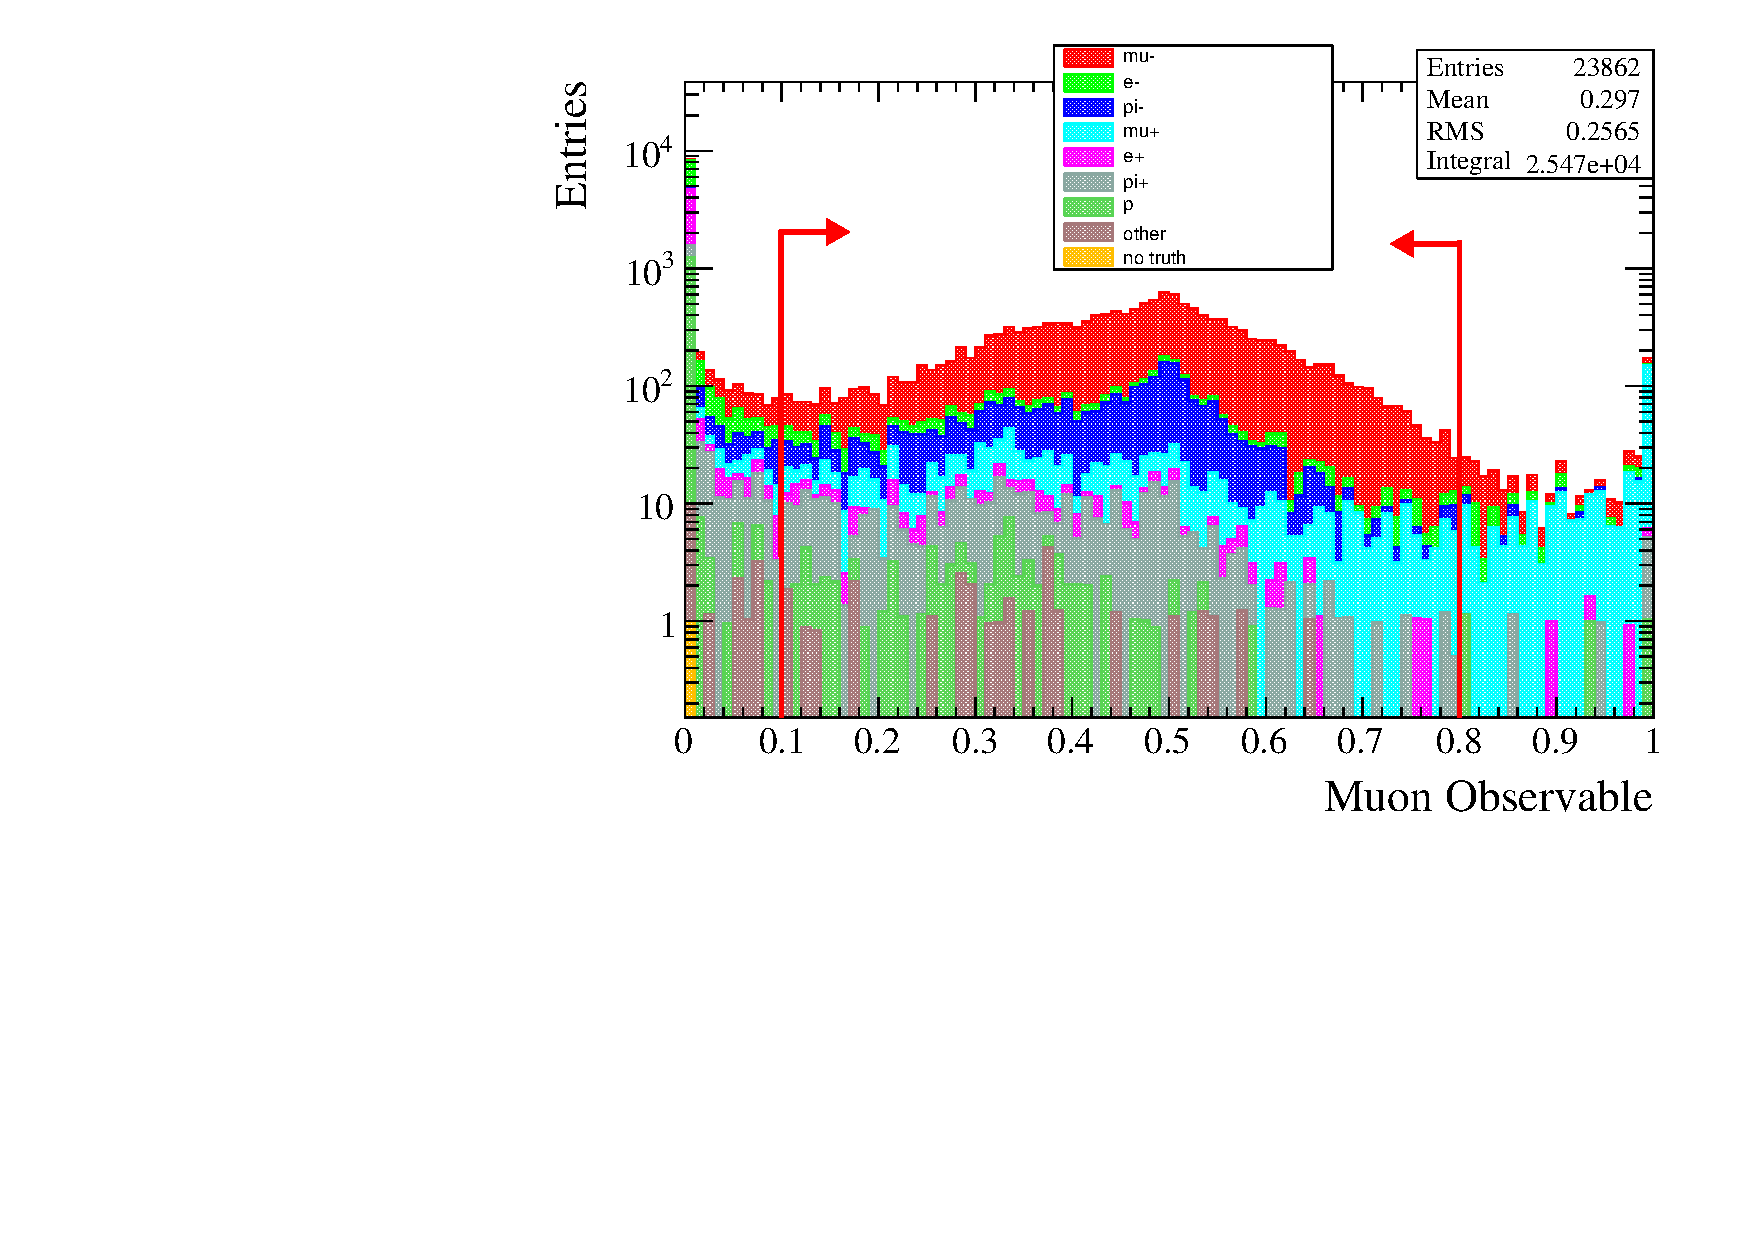
\includegraphics[width=\textwidth]{figures/numu/Cuts/numu_in_numubar/MuonLikelihood_prod6B_NuMuCont_FGD1Only}
		\caption{$\mathcal{L}_\mu$}
	\end{subfigure}
	\begin{subfigure}[t]{0.49\textwidth}
		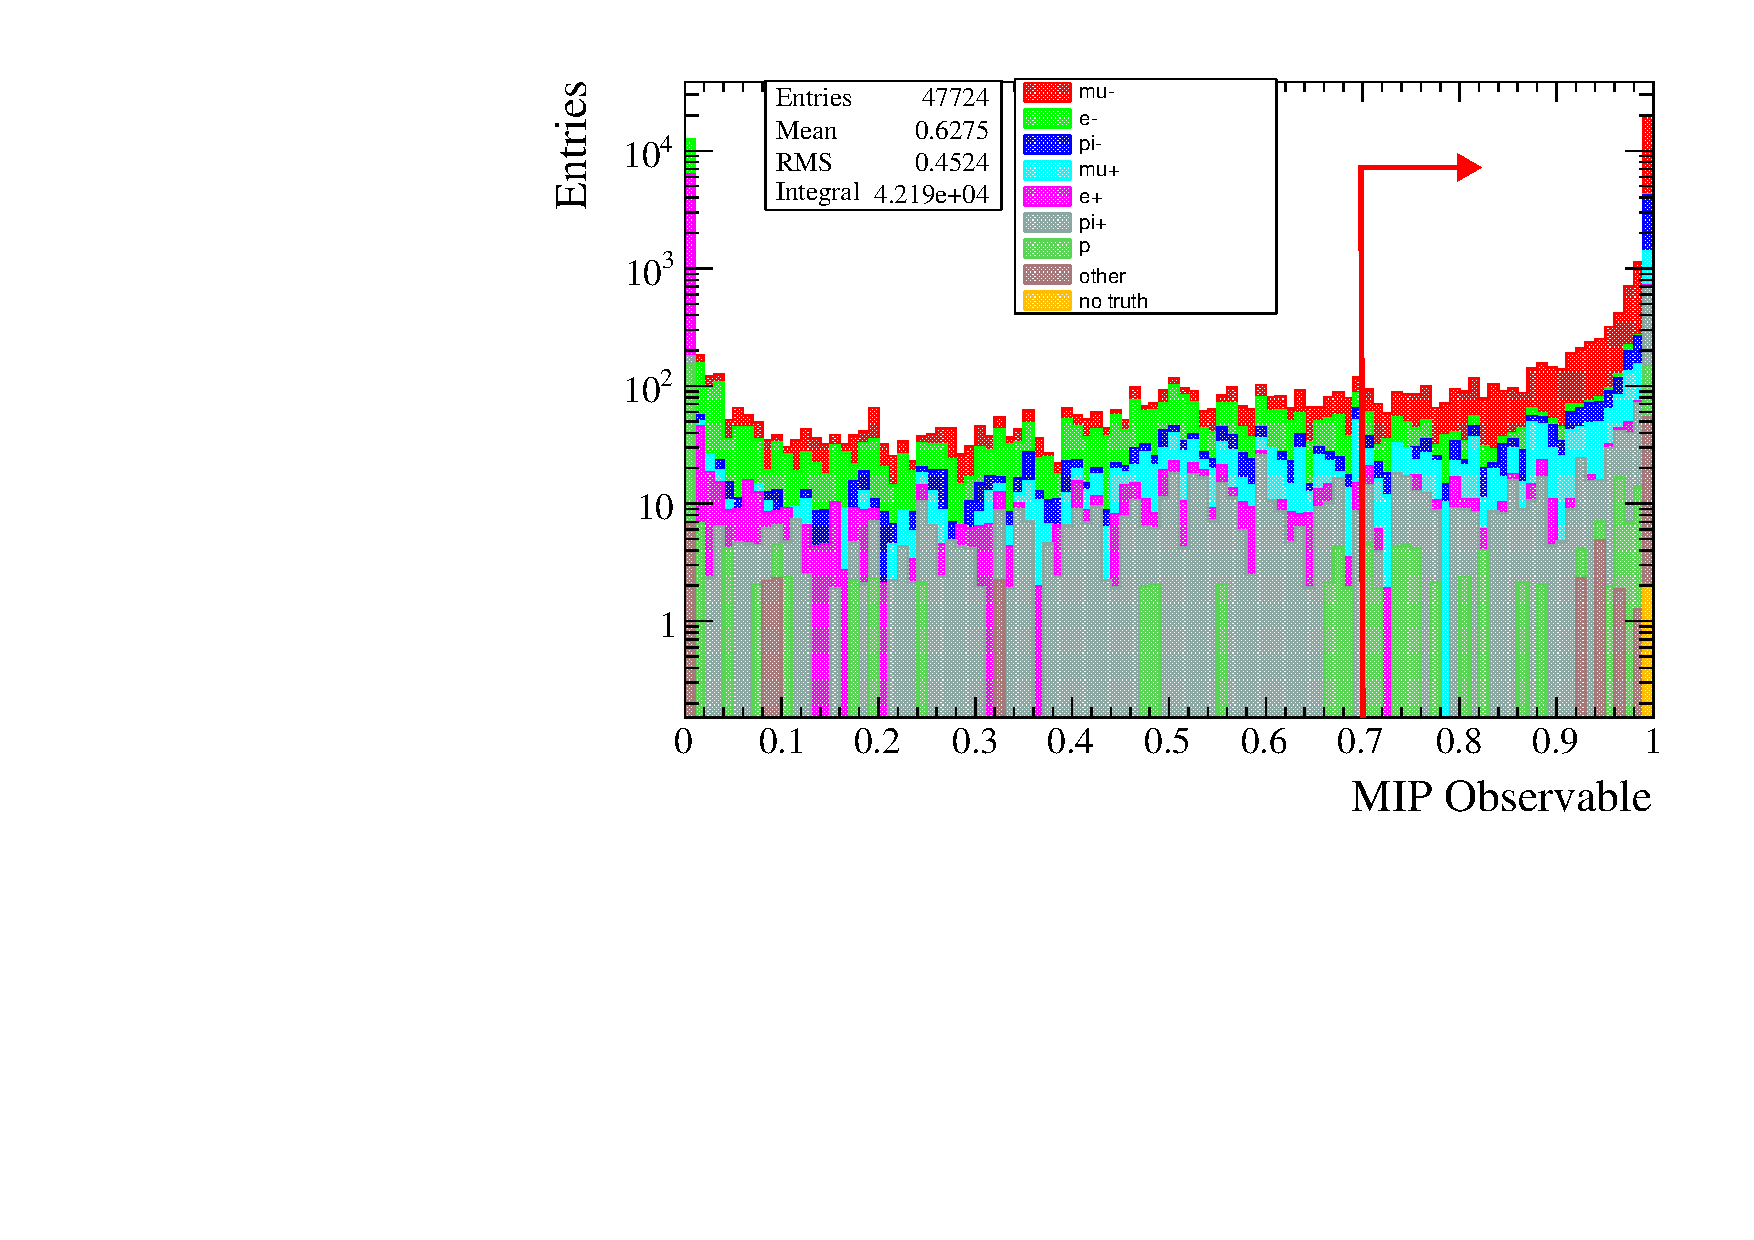
\includegraphics[width=\textwidth]{figures/numu/Cuts/numu_in_numubar/MipLikelihood_LogScale}
		\caption{$\mathcal{L}_{MIP}$}
	\end{subfigure}
	\caption{Likelihood distributions for $\mu$ and MIP using run5+6 \numubar data, used in \numu in RHC selections}
	\label{fig:nu_numubar_likelihood}
\end{figure}

The \numu in RHC selection then breaks down the CC-inclusive selection into CC1Track and CCNTrack, based entirely on the number of TPC-FGD matched tracks. Events with one such reconstructed track enters the CC1Track selection, and events with any other number of tracks regardless of PID, enter the CCNTrack selection. Hence the \numu RHC selection is analogous to the \numubar RHC selection.

\paragraph{Efficiency and purity}
As in previous sections we now study the muon tagging efficiency and topological purity of the final \numu in RHC selections.

\autoref{fig:ccnubarnu1trk_topology} shows the purity of the CC1Track selection, where we note a poor purity at low momentum, plateauing at 60\% at 0.8 GeV/c, averaging at 52\%. The overall \numu CCNtrack contribution is 29\%, 10 percentage units larger than for \numubar and is roughly constant over the full range. The wrong-sign contribution is 10\% in total, and NC is 10\%. The wrong-sign and NC contributions happen primarily at low momentum and vanish above $p_{reco}=1\text{ GeV/c}$.
\begin{figure}[!h]
	\begin{subfigure}[t]{0.49\textwidth}
		\includegraphics[width=\textwidth,page=21, trim={0mm 0mm 0mm 9mm}, clip]{figures/mach3/selection/2017b_Diag_WithSelection}
		\caption{FGD1}
	\end{subfigure}
	\begin{subfigure}[t]{0.49\textwidth}
		\includegraphics[width=\textwidth,page=25, trim={0mm 0mm 0mm 9mm}, clip]{figures/mach3/selection/2017b_Diag_WithSelection}
		\caption{FGD2}
	\end{subfigure}
	\caption{Breakdown of \numu in RHC CC 1Trk selection events' true event topology for FGD1 and FGD2 }
	\label{fig:ccnubarnu1trk_topology}
\end{figure}

\autoref{fig:ccnubarnu1trk_muon} shows the muon efficiency which closely follows the pattern of the purity. The efficiency is very poor up until 300 MeV/c and then sharply rises to plateau at 95\% at 1 GeV/c. However the event distribution peaks in region of low efficiency, causing the average to be 75\%. The background varies significantly in the low momentum range: at lowest momentum it's composed of $e^\pm$ since the TPC has similar energy loss for $e$ and $\mu$ in this region. Around the event peak, 1/2-2/3 of the selected leptons are background, almost equally wrong-sign muons and both signs of pions. The $\pi^-$ background comes primarily from NC1$\pi^-$ and \numubar CC1$\pi^-$ where the muon is missed.
\begin{figure}[!h]
	\begin{subfigure}[t]{0.49\textwidth}
		\includegraphics[width=\textwidth,page=22, trim={0mm 0mm 0mm 9mm}, clip]{figures/mach3/selection/2017b_Diag_WithSelection}
		\caption{FGD1}
	\end{subfigure}
	\begin{subfigure}[t]{0.49\textwidth}
		\includegraphics[width=\textwidth,page=26, trim={0mm 0mm 0mm 9mm}, clip]{figures/mach3/selection/2017b_Diag_WithSelection}
		\caption{FGD2}
	\end{subfigure}
	\caption{Breakdown of \numu in RHC CC 1Trk selection events' true lepton candidate for FGD1 and FGD2 }
	\label{fig:ccnubarnu1trk_muon}
\end{figure}

For the NTrack distribution purity in \autoref{fig:ccnubarnuNtrk_topology} we approximately 60\% purity, which plateaus at 70\% above 1.5 GeV/c. The largest background is from same-sign CC1Trk where a broken track or secondary interaction creates a false second (or more) track associated with the vertex. The NC contribution is approximately same size and shape to the wrong-sign CCNTrk, at 10\%, largest below $p_{reco}\sim 1\text{ GeV/c}$. For NC the contribution comes from reconstructing a \{$\pi^-$,$\pi^{0,+}$\} pair as a \{$\mu^-$, $\pi^{0,+}$\} pair, and the wrong sign NTrack comes from \{$\mu^+$, $\pi^-$\} as \{$\pi^+$, $\mu^-$\}, just as in the \numubar RHC selection, for which the NC contamination was 14\% and wrong-sign NTrack was 27\%. However, the \numubar RHC CCNtrack selection additionally stands the risk of a proton being reconstructed as the $\mu^+$, which is why the purity is worse.
\begin{figure}[!h]
	\begin{subfigure}[t]{0.49\textwidth}
		\includegraphics[width=\textwidth,page=23, trim={0mm 0mm 0mm 9mm}, clip]{figures/mach3/selection/2017b_Diag_WithSelection}
		\caption{FGD1}
	\end{subfigure}
	\begin{subfigure}[t]{0.49\textwidth}
		\includegraphics[width=\textwidth,page=27, trim={0mm 0mm 0mm 9mm}, clip]{figures/mach3/selection/2017b_Diag_WithSelection}
		\caption{FGD2}
	\end{subfigure}
	\caption{Breakdown of \numu in RHC CC NTrk selection events' true event topology for FGD1 and FGD2 }
	\label{fig:ccnubarnuNtrk_topology}
\end{figure}

Inspecting the muon tagging efficiency in \autoref{fig:ccnubarnuNtrk_muon}, we observe several traits common with the \numubar CCNTrack and \numu CCOther selections: at low momentum the lepton tag is primarily from $e^-$ due to the similar energy loss of $e$, $\mu$ and $\pi$ in this region; as we increase lepton candidate momentum we create $\mu$,$\pi$ systems in which the $\pi^-$ has the higher momentum and is assumed the $\mu^-$ candidate. The efficiency rises sharply at 0.3 GeV/c and plateaus at 80\% above 1 GeV/c, coinciding with the event distribution peak. Over the entire range the efficiency is 74\% and the $\pi^-$ background is 20\%.
\begin{figure}[!h]
	\begin{subfigure}[t]{0.49\textwidth}
		\includegraphics[width=\textwidth,page=24, trim={0mm 0mm 0mm 9mm}, clip]{figures/mach3/selection/2017b_Diag_WithSelection}
		\caption{FGD1}
	\end{subfigure}
	\begin{subfigure}[t]{0.49\textwidth}
		\includegraphics[width=\textwidth,page=28, trim={0mm 0mm 0mm 9mm}, clip]{figures/mach3/selection/2017b_Diag_WithSelection}
		\caption{FGD2}
	\end{subfigure}
	\caption{Breakdown of \numu in RHC CC NTrk selection events' true lepton candidate for FGD1 and FGD2 }
	\label{fig:ccnubarnuNtrk_muon}
\end{figure}

A summary of all selections' efficiency and purities is shown in \autoref{tab:eff_pur_summary}.
\begin{table}[!h]
	\centering
	\begin{tabular}{ l | c c }
		\hline
		\hline
		Selection 					   & Efficiency (\%) & Purity (\%) \\ 
		\hline
		\FGDCCNoPi{1}{\numu}           & 93.8  & 75.5  \\% \hline
		\FGDCCNoPi{2}{\numu}           & 93.2  & 73.5  \\% \hline
		\hline
		\FGDCCOnePi{1}{\numu}          & 83.3  & 58.0  \\% \hline
		\FGDCCOnePi{2}{\numu}          & 83.1  & 57.1  \\% \hline
		\hline
		\FGDCCOther{1}{\numu}          & 73.0  & 65.3  \\% \hline
		\FGDCCOther{2}{\numu}          & 73.4  & 64.9  \\% \hline
		\hline
		\FGDCCOneTrk{1}{\numubar}      & 90.0  & 76.7  \\% \hline
		\FGDCCOneTrk{2}{\numubar}      & 89.6  & 76.7  \\% \hline
		\hline
		\FGDCCNTrk{1}{\numubar}   	   & 54.1  & 45.1  \\% \hline
		\FGDCCNTrk{2}{\numubar}        & 53.8  & 43.9  \\% \hline
		\hline
		\FGDCCOneTrk{1}{\numu} in RHC  & 76.5  & 52.2  \\% \hline
		\FGDCCOneTrk{2}{\numu} in RHC  & 74.9  & 51.8  \\% \hline
		\hline
		\FGDCCNTrk{1}{\numu} in RHC    & 73.9  & 60.9  \\% \hline
		\FGDCCNTrk{2}{\numu} in RHC    & 74.2  & 61.4  \\% \hline
		\hline
		\hline
	\end{tabular}
	\caption{Efficiency and purity summary for all selections with the range $0 < p_{reco} < 3\text{ GeV/c}$}
	\label{tab:eff_pur_summary}
\end{table}

\section{Binning}
We expect largely similar kinematics across the two FGDs so apply the same binning in reconstructed muon momentum, \pmu, and cosine of the neutrino-muon angle, \cosmu. The binning for the fit is primarily influenced by MC statistics: we require $\sim 20$ raw MC events per bin (roughly equivalent to 1-2 data events). The momentum resolution is $\sim50\text{ MeV}$ up to 1 GeV and the angular resolution $\sim 2\degree$.
\begin{itemize}
	\item FGD1+2  CC$0\pi$, CC1$\pi$ and CCOther \numu: \\
	\pmu: 0, 300, 400, 500, 600, 700, 800, 900, 1000, 1250, 1500, 2000, 3000 (not for CC1$\pi$), 5000, 30000\\
	\cosmu:  -1, 0.6, 0.7, 0.8, 0.85, 0.9, 0.92, 0.94, 0.96, 0.98, 0.99, 1
	
	\item \FGDCCOneTrk{1+2}{\numubar}: \\
	\pmu: 0, 400, 500, 600, 700, 800, 900, 1100, 1400, 2000, 10000\\
	\cosmu: -1.0, 0.6, 0.7, 0.8, 0.85, 0.88, 0.91, 0.93, 0.95, 0.96, 0.97, 0.98, 0.99, 1
	
	\item \FGDCCNTrk{1+2}{\numubar}: \\
	\pmu: 0, 700, 950, 1200, 1500, 2000, 3000, 10000\\
	\cosmu: -1.0, 0.75, 0.85, 0.88, 0.91, 0.93, 0.95, 0.96, 0.97, 0.98, 0.99, 1
	
	\item \FGDCCnuOneTrk{1+2}{\numu} in RHC: \\
	\pmu: 0, 400, 600, 800, 1100, 2000, 10000 \\
	\cosmu: -1.0, 0.7, 0.8, 0.85, 0.9, 0.93, 0.95, 0.96, 0.97, 0.98, 0.99, 1
	
	\item \FGDCCnuNTrk{1+2}{\numu} in RHC: \\
	\pmu: 0, 500, 700, 1000, 1500, 2000, 3000, 10000\\
	\cosmu: -1.0, 0.7, 0.8, 0.85, 0.9, 0.93, 0.95, 0.96, 0.97, 0.98, 0.99, 1
\end{itemize}

The raw Monte-Carlo \pmu \cosmu event distributions with aforementioned binning is shown in \autoref{fig:nominal_mc2d} with the projections and by-mode distributions in \autoref{fig:nominal_mcpmu} and \autoref{fig:nominal_mccosmu}. The 2D plots include lines of constant $Q^2_{\text{reco}}$, for $E_\nu = 0.6 \text{ GeV}$, defined as the reconstructed (observed) $Q^2$:
\begin{equation}
Q^2_{\text{reco}} = -m^2_\mu + 2E_\nu \left( E_\mu-p_\mu\cos\theta_\mu \right)
\end{equation}
which if looking at constant $Q^2_{\text{reco}}$ surfaces with fixed $E_\nu$ leads to a simple update scheme of
\begin{equation}
\cos\theta_{\mu, 2} = \frac{\sqrt{p_{\mu,2}^2+m_{\mu,2}^2} - \sqrt{p_{\mu,1}^2+m_{\mu,1}^2}+p_{\mu,1}\cos\theta_{\mu,1}}{p_{\mu,2}}
\end{equation}
As expected from the neutrino flux at ND280 and neutrino interaction cross-sections, the CC0$\pi$ selection is an order of magnitude more populated than the other \numu selections. CC1$\pi$ and CCOther have similar statistics, and FGD1 generally has marginally more events than FGD2, owing to the reconstruction effects discussed in \autoref{sec:ND280:sel}. The \numubar CC1Track selections have similar statistics to \numu CC1$\pi$ and CCOther, a factor five higher than \numubar CCNTrack. The \numu in RHC selections have similar statistics to the \numubar CCNTrack and roughly the same for 1Track and NTrack. All the selections focus in on the $Q^2$ range of $0.1 < Q^2 < 0.5 \text{ GeV}^2$.
\begin{figure}[!h]
\begin{subfigure}[t]{0.32\textwidth}
\includegraphics[width=\textwidth,page=1]{{figures/mach3/selection/2017b_nominal_withdebug_forthesis_noweightsapplied_onlyMCnom}}
\end{subfigure}
\begin{subfigure}[t]{0.32\textwidth}
\includegraphics[width=\textwidth,page=2]{{figures/mach3/selection/2017b_nominal_withdebug_forthesis_noweightsapplied_onlyMCnom}}
\end{subfigure}
\begin{subfigure}[t]{0.32\textwidth}
\includegraphics[width=\textwidth,page=3]{{figures/mach3/selection/2017b_nominal_withdebug_forthesis_noweightsapplied_onlyMCnom}}
\end{subfigure}

\begin{subfigure}[t]{0.32\textwidth}
\includegraphics[width=\textwidth,page=4]{{figures/mach3/selection/2017b_nominal_withdebug_forthesis_noweightsapplied_onlyMCnom}}
\end{subfigure}
\begin{subfigure}[t]{0.32\textwidth}
\includegraphics[width=\textwidth,page=5]{{figures/mach3/selection/2017b_nominal_withdebug_forthesis_noweightsapplied_onlyMCnom}}
\end{subfigure}
\begin{subfigure}[t]{0.32\textwidth}
\includegraphics[width=\textwidth,page=6]{{figures/mach3/selection/2017b_nominal_withdebug_forthesis_noweightsapplied_onlyMCnom}}
\end{subfigure}

\begin{subfigure}[t]{0.24\textwidth}
\includegraphics[width=\textwidth,page=7]{{figures/mach3/selection/2017b_nominal_withdebug_forthesis_noweightsapplied_onlyMCnom}}
\end{subfigure}
\begin{subfigure}[t]{0.24\textwidth}
\includegraphics[width=\textwidth,page=8]{{figures/mach3/selection/2017b_nominal_withdebug_forthesis_noweightsapplied_onlyMCnom}}
\end{subfigure}
\begin{subfigure}[t]{0.24\textwidth}
\includegraphics[width=\textwidth,page=9]{{figures/mach3/selection/2017b_nominal_withdebug_forthesis_noweightsapplied_onlyMCnom}}
\end{subfigure}
\begin{subfigure}[t]{0.24\textwidth}
\includegraphics[width=\textwidth,page=10]{{figures/mach3/selection/2017b_nominal_withdebug_forthesis_noweightsapplied_onlyMCnom}}
\end{subfigure}

\begin{subfigure}[t]{0.24\textwidth}
\includegraphics[width=\textwidth,page=11]{{figures/mach3/selection/2017b_nominal_withdebug_forthesis_noweightsapplied_onlyMCnom}}
\end{subfigure}
\begin{subfigure}[t]{0.24\textwidth}
\includegraphics[width=\textwidth,page=12]{{figures/mach3/selection/2017b_nominal_withdebug_forthesis_noweightsapplied_onlyMCnom}}
\end{subfigure}
\begin{subfigure}[t]{0.24\textwidth}
\includegraphics[width=\textwidth,page=13]{{figures/mach3/selection/2017b_nominal_withdebug_forthesis_noweightsapplied_onlyMCnom}}
\end{subfigure}
\begin{subfigure}[t]{0.24\textwidth}
\includegraphics[width=\textwidth,page=14]{{figures/mach3/selection/2017b_nominal_withdebug_forthesis_noweightsapplied_onlyMCnom}}
\end{subfigure}
\caption{Raw Monte-Carlo event distributions for the 6CC\numu, 4CC\numubar and 4CC\numu in RHC, selections at ND280 in \pmu \cosmu. Red lines are regions of constant $Q^2_{\text{reco}}$ with fixed $E_\nu=0.6\text{ GeV}$.}
\label{fig:nominal_mc2d}
\end{figure}

\autoref{fig:nominal_mcpmu} and \autoref{fig:nominal_mccosmu} show the projections onto \pmu and \cosmu along with the composition by mode. \autoref{tab:nominal_mode} gives the mode breakdown of the histograms binned into 2D. The CC0$\pi$ samples have sizeable contributions from single pion interactions which is more than an effect from misreconstruction: in \autoref{fig:cc0pi_topology} the fraction of CC1$\pi$ topology events reconstructed as CC0$\pi$ was $\sim11\%$, whereas for the true interaction mode we have $\sim20\%$. This effect is almost entirely driven by final-state-interactions, in which nucleons and pions exit the nucleon-level interaction and are propagated through the nucleus with a probability of re-interaction with surrounding nucleons. A CC1$\pi^{0,+}$ interaction can see a pion absorbed, leaving only the outgoing muon, classifying it (correctly) as a CC0$\pi$ topology. This applies to all samples: feed-down occurs from pion absorption and feed-up occurs from inelastic nucleon or pion interactions, in which additional pions exit the nucleus. There is no effort to disentangle the effects of the fundamental interaction to that of final-state-interaction in this fit, as doing so is very model dependent\red{maybe cite some model dependence?}. In general, the selections perform well in separating the interaction models achieving above 65\% content for all samples. 

\autoref{fig:nominal_mcpmu} shows the fraction of single pion events in 0$\pi$ is highest at low momentum, reaching 50\% in the first bin. We also note the NC contribution is primarily focused in the 500-1000 MeV/c region for the 1$\pi$ and Other samples. It is also clear that the Other sample produces higher momentum muons, and mostly contains multi-$\pi$ and DIS events, as intended. 

Looking at the \cosmu projection in \autoref{fig:nominal_mccosmu}, the forward region of the CC0$\pi$ selection contains a large fraction of CC1$\pi$ events (50\%) and the highest amount of 2p2h. For the 1$\pi$ selection we note the CC coherent contribution almost exclusively in the most forward-going bin, as expected.
\begin{table}
	\begin{tabular}{l | c c c c c c | c}
		\hline
		\hline
		Sample 			& CCQE & 2p2h & CC1$\pi^{\pm,0}$ 	& CC coh 	& CC multi-$\pi$ & CC DIS  	& NC \\
		\hline
		FGD1 0$\pi$	    & \textbf{58.0} & \textbf{10.1} & 19.6 & 0.3 & 4.2 & 4.6 & 3.1 \\
		FGD2 0$\pi$	    & \textbf{56.5} & \textbf{9.5}  & 21.3 & 0.3 & 4.6 & 4.7 & 3.1 \\
		\hline
		FGD1 1$\pi$	    & 5.6 & 0.9 & \textbf{50.8} & \textbf{2.8} & \textbf{17.7} & 16.1 & 6.0 \\
		FGD2 1$\pi$	    & 5.7 & 0.8 & \textbf{50.1} & \textbf{2.9} & \textbf{17.9} & 16.5 & 5.9 \\
		\hline
		FGD1 Other	    & 5.0 & 1.0 & 15.6 & 0.4 & \textbf{26.3} & \textbf{43.7} & 7.9 \\
		FGD2 Other	    & 5.3 & 1.1 & 16.3 & 0.4 & \textbf{25.8} & \textbf{43.6} & 7.6 \\
		\hline
		FGD1 1Trk	    	& \textbf{64.2} & \textbf{10.1} & 15.0 & 0.7 & 2.9 & 2.5 & 4.5 \\
		FGD2 1Trk	    	& \textbf{64.4} & \textbf{9.9} & 15.0 & 0.7 & 2.9 & 2.5 & 4.6 \\
		\hline
		FGD1 NTrk	    	& 7.8 & 2.7 & \textbf{29.3} & \textbf{3.4} & \textbf{20.3} & \textbf{26.0} & 10.5 \\ 
		FGD2 NTrk	  		& 8.7 & 2.6 & \textbf{29.0} & \textbf{3.3} & \textbf{20.5} & \textbf{25.4} & 10.5 \\
		\hline
		FGD1 1Trk   \numu 	& \textbf{44.5} & \textbf{8.5} & 25.4 & 0.9 & 7.2 & 6.2 & 7.5 \\
		FGD2 1Trk	\numu   & \textbf{43.8} & \textbf{8.3} & 25.5 & 0.8 & 7.7 & 6.6 & 7.2 \\
		FGD1 NTrk	\numu   & 12.6 & 3.1 & \textbf{29.3} & \textbf{1.8} & \textbf{20.9} & \textbf{25.6} & 6.6 \\ 
		\hline
		FGD2 NTrk	\numu   & 12.2 & 2.8 & \textbf{30.0} & \textbf{1.9} & \textbf{21.3} & \textbf{25.6} & 6.2 \\
		\hline
		\hline
	\end{tabular}
	\caption{Percentage mode breakdown for the binned nominal \textbf{unscaled} Monte-Carlo samples, \textbf{boldface} indicates interactions targeted by specific selections. The distributions are \textbf{not} bin-width normalised. Compare to \autoref{tab:nominal_mode_afterscale} for effect of weights.}
	\label{tab:nominal_mode}
\end{table}

\begin{figure}[!h]
	\begin{subfigure}[t]{0.24\textwidth}
		\includegraphics[width=\textwidth,page=15]{{figures/mach3/selection/2017b_nominal_withdebug_forthesis_noweightsapplied_onlyMCnom}}
	\end{subfigure}
	\begin{subfigure}[t]{0.24\textwidth}
		\includegraphics[width=\textwidth,page=16]{{figures/mach3/selection/2017b_nominal_withdebug_forthesis_noweightsapplied_onlyMCnom}}
	\end{subfigure}
	\begin{subfigure}[t]{0.24\textwidth}
		\includegraphics[width=\textwidth,page=18]{{figures/mach3/selection/2017b_nominal_withdebug_forthesis_noweightsapplied_onlyMCnom}}
	\end{subfigure}
	\begin{subfigure}[t]{0.24\textwidth}
		\includegraphics[width=\textwidth,page=20]{{figures/mach3/selection/2017b_nominal_withdebug_forthesis_noweightsapplied_onlyMCnom}}
	\end{subfigure}

	\begin{subfigure}[t]{0.24\textwidth}
		\includegraphics[width=\textwidth,page=22]{{figures/mach3/selection/2017b_nominal_withdebug_forthesis_noweightsapplied_onlyMCnom}}
	\end{subfigure}
	\begin{subfigure}[t]{0.24\textwidth}
		\includegraphics[width=\textwidth,page=24]{{figures/mach3/selection/2017b_nominal_withdebug_forthesis_noweightsapplied_onlyMCnom}}
	\end{subfigure}
	\begin{subfigure}[t]{0.24\textwidth}
		\includegraphics[width=\textwidth,page=26]{{figures/mach3/selection/2017b_nominal_withdebug_forthesis_noweightsapplied_onlyMCnom}}
	\end{subfigure}

	\begin{subfigure}[t]{0.24\textwidth}
		\includegraphics[width=\textwidth,page=28]{{figures/mach3/selection/2017b_nominal_withdebug_forthesis_noweightsapplied_onlyMCnom}}
	\end{subfigure}
	\begin{subfigure}[t]{0.24\textwidth}
		\includegraphics[width=\textwidth,page=30]{{figures/mach3/selection/2017b_nominal_withdebug_forthesis_noweightsapplied_onlyMCnom}}
	\end{subfigure}
	\begin{subfigure}[t]{0.24\textwidth}
		\includegraphics[width=\textwidth,page=32]{{figures/mach3/selection/2017b_nominal_withdebug_forthesis_noweightsapplied_onlyMCnom}}
	\end{subfigure}
	\begin{subfigure}[t]{0.24\textwidth}
		\includegraphics[width=\textwidth,page=34]{{figures/mach3/selection/2017b_nominal_withdebug_forthesis_noweightsapplied_onlyMCnom}}
	\end{subfigure}

	\begin{subfigure}[t]{0.24\textwidth}
		\includegraphics[width=\textwidth,page=36]{{figures/mach3/selection/2017b_nominal_withdebug_forthesis_noweightsapplied_onlyMCnom}}
	\end{subfigure}
	\begin{subfigure}[t]{0.24\textwidth}
		\includegraphics[width=\textwidth,page=38]{{figures/mach3/selection/2017b_nominal_withdebug_forthesis_noweightsapplied_onlyMCnom}}
	\end{subfigure}
	\begin{subfigure}[t]{0.24\textwidth}
		\includegraphics[width=\textwidth,page=40]{{figures/mach3/selection/2017b_nominal_withdebug_forthesis_noweightsapplied_onlyMCnom}}
	\end{subfigure}
	\begin{subfigure}[t]{0.24\textwidth}
		\includegraphics[width=\textwidth,page=42]{{figures/mach3/selection/2017b_nominal_withdebug_forthesis_noweightsapplied_onlyMCnom}}
	\end{subfigure}
	\caption{Raw Monte-Carlo event distributions for the 6CC\numu, 4CC\numubar and 4CC\numu in RHC, selections at ND280 projected onto \pmu and bin-width normalised}
	\label{fig:nominal_mcpmu}
\end{figure}

\begin{figure}[!h]
	\begin{subfigure}[t]{0.24\textwidth}
		\includegraphics[width=\textwidth,page=15]{{figures/mach3/selection/2017b_nominal_withdebug_forthesis_noweightsapplied_onlyMCnom}}
	\end{subfigure}
	\begin{subfigure}[t]{0.24\textwidth}
		\includegraphics[width=\textwidth,page=17]{{figures/mach3/selection/2017b_nominal_withdebug_forthesis_noweightsapplied_onlyMCnom}}
	\end{subfigure}
	\begin{subfigure}[t]{0.24\textwidth}
		\includegraphics[width=\textwidth,page=19]{{figures/mach3/selection/2017b_nominal_withdebug_forthesis_noweightsapplied_onlyMCnom}}
	\end{subfigure}
	\begin{subfigure}[t]{0.24\textwidth}
		\includegraphics[width=\textwidth,page=21]{{figures/mach3/selection/2017b_nominal_withdebug_forthesis_noweightsapplied_onlyMCnom}}
	\end{subfigure}
	
	\begin{subfigure}[t]{0.24\textwidth}
		\includegraphics[width=\textwidth,page=23]{{figures/mach3/selection/2017b_nominal_withdebug_forthesis_noweightsapplied_onlyMCnom}}
	\end{subfigure}
	\begin{subfigure}[t]{0.24\textwidth}
		\includegraphics[width=\textwidth,page=25]{{figures/mach3/selection/2017b_nominal_withdebug_forthesis_noweightsapplied_onlyMCnom}}
	\end{subfigure}
	\begin{subfigure}[t]{0.24\textwidth}
		\includegraphics[width=\textwidth,page=27]{{figures/mach3/selection/2017b_nominal_withdebug_forthesis_noweightsapplied_onlyMCnom}}
	\end{subfigure}

	\begin{subfigure}[t]{0.24\textwidth}
		\includegraphics[width=\textwidth,page=29]{{figures/mach3/selection/2017b_nominal_withdebug_forthesis_noweightsapplied_onlyMCnom}}
	\end{subfigure}
	\begin{subfigure}[t]{0.24\textwidth}
		\includegraphics[width=\textwidth,page=31]{{figures/mach3/selection/2017b_nominal_withdebug_forthesis_noweightsapplied_onlyMCnom}}
	\end{subfigure}
	\begin{subfigure}[t]{0.24\textwidth}
		\includegraphics[width=\textwidth,page=33]{{figures/mach3/selection/2017b_nominal_withdebug_forthesis_noweightsapplied_onlyMCnom}}
	\end{subfigure}
	\begin{subfigure}[t]{0.24\textwidth}
		\includegraphics[width=\textwidth,page=35]{{figures/mach3/selection/2017b_nominal_withdebug_forthesis_noweightsapplied_onlyMCnom}}
	\end{subfigure}

	\begin{subfigure}[t]{0.24\textwidth}
		\includegraphics[width=\textwidth,page=37]{{figures/mach3/selection/2017b_nominal_withdebug_forthesis_noweightsapplied_onlyMCnom}}
	\end{subfigure}
	\begin{subfigure}[t]{0.24\textwidth}
		\includegraphics[width=\textwidth,page=39]{{figures/mach3/selection/2017b_nominal_withdebug_forthesis_noweightsapplied_onlyMCnom}}
	\end{subfigure}
	\begin{subfigure}[t]{0.24\textwidth}
		\includegraphics[width=\textwidth,page=41]{{figures/mach3/selection/2017b_nominal_withdebug_forthesis_noweightsapplied_onlyMCnom}}
	\end{subfigure}
	\begin{subfigure}[t]{0.24\textwidth}
		\includegraphics[width=\textwidth,page=43]{{figures/mach3/selection/2017b_nominal_withdebug_forthesis_noweightsapplied_onlyMCnom}}
	\end{subfigure}
	\caption{Raw Monte-Carlo event distributions for the 6CC\numu, 4CC\numubar and 4CC\numu in RHC, selections at ND280 projected onto \cosmu and bin-width normalised}
	\label{fig:nominal_mccosmu}
\end{figure}


\section{Systematics}
\label{sec:syst}
The fit's main goal is to minimise impact of systematic parameters for T2K-SK oscillation analyses by using near-detector data. The shared parameters between ND280 and SK are the neutrino flux parameters (since T2K and SK are in the same neutrino ``beamline''), and neutrino-nucleus interaction parameters. Nuisance parameters are mostly ND280 detector parameters and cross-section parameters that are parametrised as only effective on Carbon. As such, there are many ``parameters of interest'', which the following sections cover.

\subsection{Flux}
\label{subsec:syst_flux}
The flux systematics are evaluated by varying underlying parameters in the flux model and using NA61/SHINE \red{CITE} data. [7] N. Antoniou et al. CERN-SPSC-2006-034, 2006.

The NA61 data comes from runs using the thin target, whereas the T2K target is roughly 2 interaction lengths The data is $\pi^\pm$, $K^\pm$, $K^0_S$ and $\rho^+$.

HARP data used for pion rescattering.

Talk about the corrections in psyche
\begin{itemize}
  \item ND280, SK FHC \numu; ND280, SK RHC \numubar, :\\
    $E_\nu^{true}$: 0, 0.4, 0.5, 0.6, 0.7, 1, 1.5, 2.5, 3.5, 5, 7, 30

  \item ND280, SK FHC \numubar; ND280, SK RHC \numu:\\
    $E_\nu^{true}$: 0, 0.7, 1, 1.5, 2.5, 30

  \item ND280, SK FHC \nue; ND280, SK RHC \nuebar:\\
    $E_\nu^{true}$: 0, 0.5, 0.7, 0.8, 1.5, 2.5, 4, 30

  \item ND280, SK FHC \nuebar; ND280, SK RHC \nue:\\
    $E_\nu^{true}$: 0, 2.5, 30
\end{itemize}

\subsection{Detector systematics}
\label{subsec:syst_nd280}
The treatment of ND280 detector systematic uncertainties consists of varying the underlying detector systematics, such as TPC PID, FGD PID, TPC Momentum scale\red{talk about all the detector systematics in summary} and study the impact on the number of predicted events in each \pmu \cosmu bin. 

There are three categories of underlying ND280 systematics: observable-variation systematics, efficiency like systematics, normalisation systematic

The event variation in each \pmu \cosmu bin is assumed to be Gaussian \red{show examples of good Gaussian bins and bad ones} 

see TN 212 p 95
Field distortions
Momentum resolution
Momentum scale
TPC PID
FGD PID
Time of flight

charge ID efficiency
tpc cluster eff
tpc track eff
fgd track eff
tpc-fgd matching eff
michel electron
oofv bckg
pile-up
fgd mass
pion SI

all magnet
sand muon bkgd
total

read p39 onwards about syst

The number of detector systematics still decreased slightly from 580 to 556 due to merging bins with similar detector systematic effects for the rebinned samples.
All the consecutive bins with similar systematic values have been merged in order to reach a lower number of parameters (556) while the number of bins in the fit increased a lot (1624 bins), keeping the number of parameters under control.
It has been demonstrated with Asimov fits, the results of which are shown in \autoref{fig:2017_rebin_asimov}, that the effect of this rebinning was small.

The effect of changing the ND280 systematics binning was done with an older cross-section model than which the fit was completed in. This was due to a late delivery of the cross-section model \red{write an appendix on this model}. The flux parameters were entirely consistent.
\begin{table}
	\centering
	\begin{tabular}{ l | c | c }
		\hline
		Parameter & Fit binning & Similar syst. merge \\
		\hline
		\hline
		FSI INEL LO & $0.0 \pm 0.202$ & $0.0\pm0.200$ \\
		FSI INEL HI & $0.0 \pm 0.235$ & $0.0\pm0.233$ \\
		FSI PI PROD & $0.0 \pm 0.347$ & $0.0\pm0.344$ \\
		FSI CEX LO  & $0.0 \pm 0.416$ & $0.0\pm0.412$ \\
		FSI CEX HI  & $0.0 \pm 0.193$ & $0.0\pm0.191$ \\
		$M_A^{QE}$  & $1.2 \pm 0.0517$ & $1.2\pm0.0512$ \\
		$p_F^{C}$   & $217 \pm 36.96$ & $217\pm36.021$ \\
		2p2h norm C & $100 \pm 30.79$ & $100\pm30.56$ \\
		$E_B^{C}$   & $25.0 \pm 8.57$ & $25.0\pm8.56$ \\
		$p_F^{O}$   & $225 \pm 57.61$  & $225\pm56.16$ \\
		2p2h norm O & $100 \pm 277.98$ & $0.0\pm272.62$ \\
		$E_B^{C}$   & $27.0 \pm 9.00$ & $27.0\pm9.00$ \\
		$C_5^A$		& $1.01 \pm 0.066$ & $1.01\pm0.064$ \\
		$M_A^{1\pi}$ & $0.95 \pm 0.060$ & $0.95\pm0.059$ \\
		$I_{1/2}$ non-res & $1.30 \pm 0.180$ & $1.30\pm0.180$ \\
		CC $\nu_e$ norm & $1.00 \pm 0.030$ & $1.00\pm0.030$ \\
		DIS Shape	& $0.00 \pm 0.208$ & $0.0\pm0.208$ \\
		CC Coherent norm & $1.0 \pm 0.258$ & $1.0\pm0.257$ \\
		NC Coherent norm & $1.0 \pm 0.299$ & $1.0\pm0.299$ \\
		NC Other & $1.0 \pm 0.182$ & $1.0\pm0.181$ \\
		2p2h $\bar{\nu}$ & $1.0 \pm 0.332$ & $1.0\pm0.329$ \\
		\hline
	\end{tabular}
	\caption{Cross-section parameter results from comparisons using fit binning and a merged binning for the 2015 cross-section model.}
\label{fig:2017_rebin_asimov}
\end{table}

The merged systematics binning was improved to:
\begin{itemize}
	\item FHC $\nu_{\mu}$~CC0$\pi$ bin edges: \\
	\pmu (MeV/c): 0, 1000, 1250, 2000, 3000, 5000, 30000 \\
	\cosmu:  -1, 0.6, 0.7, 0.8, 0.85,0.94, 0.96, 1
	\item FHC $\nu_{\mu}$~CC1$\pi$  bin edges: \\
	\pmu (MeV/c):  0, 300, 1250, 1500, 5000, 30000 \\
	\cosmu: -1, 0.7, 0.85, 0.9, 0.92, 0.96, 0.98, 0.99, 1
	\item FHC $\nu_{\mu}$~CCOther bin edges: \\
	\pmu (MeV/c): 0, 1500, 2000, 3000, 5000, 30000 \\
	\cosmu:  -1, 0.8, 0.85, 0.9, 0.92, 0.96, 0.98, 0.99, 1
	\item RHC $\bar{\nu}_{\mu}$~CC 1-Track bin edges: \\
	\pmu (MeV/c): 0, 400, 900, 1100, 2000, 10000 \\
	\cosmu:  -1, 0.6, 0.7, 0.88, 0.95, 0.97, 0.98, 0.99, 1.00
	\item RHC $\bar{\nu}_{\mu}$~CC N-Track bin edges: \\
	\pmu (MeV/c):  0, 700, 1200, 1500, 2000, 3000, 10000 \\
	\cosmu: -1, 0.85, 0.88, 0.93, 0.98, 0.99, 1.00
	\item RHC $\nu_{\mu}$~CC 1-Track bin edges: \\
	\pmu (MeV/c):  0, 400, 800, 1100, 2000, 10000 \\
	\cosmu:   -1, 0.7, 0.85, 0.90, 0.93, 0.96, 0.98, 0.99, 1.00
	\item RHC $\nu_{\mu}$~CC N-Track bin edges: \\
	\pmu (MeV/c):  0, 1000, 1500, 2000, 3000, 10000 \\
	\cosmu: -1, 0.8, 0.90, 0.93, 0.95, 0.96, 0.97, 0.99, 1.00
\end{itemize}
Be mega clear that each of these above make up one parameter

\subsection{Cross-section}
\label{subsec:syst_xsec}
splines vs normalisation parameter, Maybe extra bit on BeRPA because of involvement

\section{Building and varying the Monte-Carlo prediction}
T2K has been taking data since 2010 with steadily increasing beam power and protons on target (POT), and is currently on ``run 9'', shown in \autoref{fig:t2k_pot}. This analysis uses data from runs 2 to 6: run 1 was omitted because parts of the detector was uninstrumented (and is only $\sim4\%$ of the run 1-6 data), and run 7 and beyond had not gone through full Monte-Carlo production until summer 2017. 

The overall efficiency of ND280 in runs 2 to 6 was approximately 85\%, collecting 9.7E20 POT out of 12E20 POT. The good POT\footnote{Defined as POT collected when all ND280 sub-detectors and global DAQ are flagged online} per run used in this analysis is listed in \autoref{tab:pot_2017}.

\begin{figure}
	\includegraphics[width=0.5\textwidth, trim={5mm 100mm 5mm 90mm}, clip]{{figures/pow_t2k_all_toRun77full}}
	\caption{T2K protons on target and beam power for run 1-9}
	\label{fig:t2k_pot}
\end{figure}

\begin{table}[htbp]
	\centering
	\begin{tabular}{ l c c c }
		\hline
		Run & Data POT (E19) & MC POT (E19) & Sand POT (E19) \\
		\hline
		\hline
		2a  FHC & 3.59337    & 92.15       & 10 \\
		2w  FHC & 4.33934    & 120.15      & 10 \\
		\hline
		3b FHC  & 2.17273    & 44.8        & 5 \\
		3c FHC  & 13.6447    & 263         & 25 \\
		\hline
		4a FHC  & 17.8271    & 349.9       & 30 \\
		4w FHC  & 16.4277    & 349.65      & 29.15 \\
		\hline
		5 RHC & 4.3468     & 208.25      & 20 \\
		\hline
		6b RHC & 12.8838    & 141.03      & 40 \\
		6c RHC & 5.07819    & 53.21       & 15 \\
		6d RHC & 7.75302    & 69.41       & 20 \\
		6e RHC & 8.51668    & 86.72       & 23 \\
		\hline
		\hline
		Total FHC & 58.00494 & 1219.65 & 109.15\\
		Total RHC & 38.57849 & 558.62  & 118 \\
		\hline
		Total & 96.58343 & 1778.27 & 227.15 \\
		\hline
	\end{tabular}
	\caption{Counted and generated proton-on-targets for the T2K ND280 2017 analysis. FHC denotes Forward Horn Current (neutrino dominated mode), RHC denotes Reverse Horn Current (anti-neutrino dominated mode)}
	\label{tab:pot_2017}
\end{table}
The Monte-Carlo is generated for the different run-periods to account for beam configurations, ND280 configurations, run-dependent calibrations, and so on. Runs marked ``a'' and ``w'' refer to the P0D detector's removable water bags being air filled (a) or water filled (w), which require different ND280 geometries in simulation.

To build the nominal distribution for direct comparison to data, a number of scalings and weights are applied. For the near-detector portion of MaCh3 and BANFF, all weights are applied on an event-by-event basis:
\begin{itemize}
	\item \textbf{POT weight:} \\
	A run-by-run scaling factor taking the ratio of total good flagged data to the generated Monte-Carlo POT. An event receives a one-time weight depending on what run it was from and how much MC was generated in the production. These numbers can be read off directly from \autoref{tab:pot_2017}. This weight $w_\text{POT}$ is only applied once and is not varied in the fit.
	
	\item \textbf{Flux weight:} \\
	A run-by-run correction to the nominal neutrino flux which the production was made in. The weight is applied as a function of $E_\nu^{true}$ with~$0 < E_\nu^{true} < 30 \text{ GeV}$~\red{show example of this, psycheND280utils/data/tuned13av2}, detailed in \autoref{subsec:syst_flux}. An event receives a weight depending on what run it was from and its $E_\nu^{true}$. The weight $w_\text{Flux}$ is only applied once and is not varied in the fit.
	
	\item \textbf{Beam covariance weight:} \\
	An event-by-event weight to vary the impact of the flux simulation. An event gets weighted as a function of the neutrino running mode (FHC or RHC), the flavour of neutrino ($\nu_\mu$, $\bar{\nu}_\mu$, $\nu_e$ or $\bar{\nu}_e$) and the neutrino energy. There are 100 parameters $\vec{b}$ in the fit---although only 50 being constrained directly by ND280 data, the remaining 50 being the SK flux parameters, constrained solely by their correlations with the ND280 flux parameters---outlined in detail in \autoref{subsec:syst_flux}.
	
	The weight $w_{\vec{b}\rightarrow \vec{b}'}$ is applied once to weight the simulation to nominal, and is recalculated for every iteration of the fit.
	
	\item \textbf{Cross-section weight:} \\
	An event-by-event weight taking the full generated event through the neutrino interaction simulation, calculating a weight to apply to the event. The applied weight is calculated as $w_{\vec{x} \rightarrow \vec{x}'}=\sigma(\vec{x}')/\sigma(\vec{x})$ for the generated neutrino interaction systematic parameter values $\vec{x}$ and the modified parameter values $\vec{x}'$. The event can receive a normalisation and a shape parameter depending on its interaction type and the interaction model considered in the analysis. Details of the model are found in \autoref{subsec:syst_xsec}.
	
	The weight $w_{\vec{x}\rightarrow \vec{x}'}$ is applied once to weight the simulation to nominal, and is recalculated for every iteration of the fit.
	
	\item \textbf{Detector covariance weight:} \\
	An event-by-event weight from the reconstruction and selection package to vary the impact of the detector simulation. It is applied as a function of the event's topology and detector (e.g. FGD1 CC0$\pi$) and which detector covariance bin the event bin falls into (e.g. $p_\mu=350\text{ MeV}, \cos\theta_\mu=0.99$). The weight is a normalisation parameter $\vec{d}$ for each bin in the detector covariance matrix scheme, explained in detail in \autoref{subsec:syst_nd280}.
	
	The weight $w_{\vec{d}\rightarrow \vec{d}'}$ is applied once to weight the simulation to nominal, and is recalculated for every iteration of the fit.
\end{itemize}

All weights are parameterised as multiplicative, so for a two parameter variation $x \rightarrow x'$ and $y \rightarrow y'$ we have the total weight 
\begin{equation}
w_{x \rightarrow x', y \rightarrow y'} = w_{x \rightarrow x', y \rightarrow y} \times w_{x \rightarrow x, y\rightarrow y'}
\end{equation}

Defining the beam parameters as $\vec{b}$, cross-section parameters as $\vec{x}$ and detector parameters as $\vec{d}$, we express one rescaled Monte-Carlo event $i$ as

\begin{equation}
\lambda_i\left(\vec{b}, \vec{x}, \vec{d}\right) = 1 \times w_i^\text{POT} \times w_i^\text{Flux} \times w^{\vec{b}\rightarrow \vec{b}'}_i \times w^{\vec{x} \rightarrow \vec{x}'}_i \times w^{\vec{d}\rightarrow \vec{d}'}_i
\label{eq:mc_scale}
\end{equation}

The effect of each weight on the MC sample statistics is shown in \autoref{tab:eventrate_mach3}. The nominal flux and detector weights are 1.0, so are not included in the table

\begin{table}[!h]
	\resizebox{\textwidth}{!}{
	\begin{tabular}{ l | c | c | c | c | c }
		\hline
		Sample & Raw MC & POT only & POT+xsec & POT+NDCov & POT+BeamCov \\ 
		\hline
		\hline
		\FGDCCNoPi{1}{\numu}& 337436 & 15905.2 & 15340.2 & 16246.1 & 16090.8 \\
		\FGDCCOnePi{1}{\numu}& 84982  & 4011.58 & 3819.3 & 4131.35 & 4058.36 \\
		\FGDCCOther{1}{\numu}& 65286 & 3071.21 & 3078.52 & 3374.21 & 3107.04 \\
		\FGDCCNoPi{2}{\numu}& 345467 & 16259.6 & 15749.8 & 16415 & 16449.2 \\
		\FGDCCOnePi{2}{\numu}& 70444  & 3318.26 & 3190.09 & 3321.4 & 3356.97 \\
		\FGDCCOther{2}{\numu}& 63402  & 2983.43 & 2995.68 & 3051.48 & 3018.22 \\
		\FGDCCOneTrk{1}{\numubar}& 54419  & 3744.02 & 3430.15 & 3872.18 & 3773.79 \\
		\FGDCCNTrk{1}{\numubar}& 15392  & 1056.8 & 986.32 & 1121.1 & 1065.2 \\
		\FGDCCOneTrk{2}{\numubar}& 55732  & 3833.73 & 3506.36 & 3906.32 & 3864.24 \\
		\FGDCCNTrk{2}{\numubar}& 15808  & 1088.15 & 1024.77 & 1122.73 & 1096.81 \\
		\FGDCCOneTrk{1}{\numu} in RHC& 18146 & 1246.03 & 1194.72 & 1262.00 & 1255.92 \\
		\FGDCCNTrk{1}{\numu} in RHC& 17156 & 1181.54 & 1172.13 & 1257.34 & 1190.94 \\
		\FGDCCOneTrk{2}{\numu} in RHC& 18052 & 1231.24 & 1189.64 & 1245.3 & 1241.02 \\
		\FGDCCNTrk{2}{\numu} in RHC& 16339 & 1127.64 & 1121.37 & 1150.7 & 1136.62 \\
		\hline
		\hline
	\end{tabular}
}
	\caption{Event rates broken by type of weight applied for the nominal MC samples}
	\label{tab:eventrate_mach3}
\end{table}

\subsection{Defining the test-statistic}
As mentioned in \autoref{sec:ND280:sel}, data and simulation events are binned in \pmu, \cosmu for 14 different selections (seven per FGD): \numu CC0$\pi$, \numu CC1$\pi$, \numu CCOther, \numubar CC1Track, \numubar CCNTrack, \numu in RHC CC1Track and \numu in RHC CCNTrack. It is assumed that the data $n^{\alpha}$ in each bin $\alpha$, is a statistical fluctuation of the simulation in that bin, $\lambda^{\alpha}$, and the probability distribution to observe $n^{\alpha}$ given $\lambda^\alpha$ is Poissonian:
\begin{equation}
P(n^\alpha|\lambda^\alpha) = \frac{e^{-\lambda^\alpha} \left(\lambda^\alpha\right)^n}{\left(n^\alpha\right)!}
\end{equation}
The Monte-Carlo prediction $\lambda$ is influenced by the beam parameters $\vec{b}$, the cross-section parameters $\vec{x}$ and the ND280 detector parameters $vec{d}$ outlined in \autoref{eq:mc_scale}. Then the statistical contribution to the negative log-likelihood per \pmu \cosmu bin $\alpha$ is
\begin{equation}
-\log\mathcal{L}^\alpha_\text{Sample} = \lambda^\alpha(\vec{b},\vec{x},\vec{d}) - n^\alpha + n^\alpha\log\frac{n^\alpha}{\lambda^\alpha(\vec{b},\vec{x},\vec{d})}
\end{equation}

The majority of systematics in \autoref{sec:syst} are constrained by prior information outside of the ND280 data used in the fit. The constraints may come from calibration studies, external cross-section data, beam simulations, and so on. A covariance matrix $\boldsymbol{V}_{i,j}$ encoding the correlations and uncertainties of parameters $i$ to $j$ is used for the separate sources of systematics. If the central values from external constraints (priors) is $\vec{\mu}$ and the parameter values varied in the fit are $\vec{X}$, we assume a Gaussian probability density function for each parameter, giving rise to a negative log-likelihood contribution for systematic $K$
\begin{equation}
-\log\mathcal{L}^K_\text{Syst} = \frac{1}{2}( X_i - \mu_i ) \left(\boldsymbol{V}^K\right)^{-1}_{i,j} ( X_j - \mu_j )
\end{equation}
and for our three separate sources of systematics we then have in total
\begin{equation}
-\log\mathcal{L_\text{Syst}} = -\left(\log\mathcal{L_\text{Flux}} + \log\mathcal{L_\text{Interaction}} + \log\mathcal{L_\text{ND280}}\right)
\end{equation}
Finally, our combined test-statistic for \pmu, \cosmu bins $\alpha$ over samples $S$, using our three sets of systematics (flux with parameters $\vec{b}$, cross-section with parameters $\vec{x}$, ND280 with parameters $\vec{d}$), is
\begin{equation}
\label{eq:test_stat}
\begin{split}
-\log\mathcal{L_\text{Total}} & =  \sum_S^\text{Samples} \left( \sum_{\alpha}^\text{Bins} \left( \lambda^\alpha(\vec{b},\vec{x},\vec{d}) - n^\alpha + n^\alpha\log\frac{n^\alpha}{\lambda^\alpha(\vec{b},\vec{x},\vec{d})} \right) \right)_S \\
 & + \frac{1}{2} \left( \sum_{i,j}^\text{Flux} ( b_i - \mu_i ) \left(\boldsymbol{V}^b\right)^{-1}_{i,j} ( b_j - \mu_j ) \right) \\
 & + \frac{1}{2} \left( \sum_{i,j}^\text{Interaction} ( x_i - \mu_i ) \left(\boldsymbol{V}^x\right)^{-1}_{i,j} ( x_j - \mu_j ) \right) \\
 & + \frac{1}{2} \left( \sum_{i,j}^\text{ND280} ( d_i - \mu_i ) \left(\boldsymbol{V}^d\right)^{-1}_{i,j} ( d_j - \mu_j ) \right)
\end{split}
\end{equation}

\section{Parameters of interest}
flux and cross-section

\section{Fitting method: MCMC}
tests

\section{Nominal model}
\label{sec:nom_model}
The rates for the data and nominal model with all mentioned Monte-Carlo scalings and selections are presented in \autoref{tab:event_rates_2017}. We note that generally the Monte-Carlo rates of the CC0$\pi$ and CC1Track are underestimated (2-3\%) , CC$1\pi$ is overestimated (6-11\%) and CCOther is under-estimated (5-15\%). \numubar selections except FGD2 CC1Track \numubar are overestimated by 5\%, with FGD1 being 2\%. The \numu in RHC selections are mildly underestimated. The rates across the FGDs are consistent for all selections.
\begin{table}[!h]
	\centering
	\begin{tabular}{ l | c c c }
		\hline
		Sample & Data & Nominal MC & Data/MC \\ \hline
		\hline
		\FGDCCNoPi{1}{\numu}           & 17136 & 16723.80 & 1.02 \\% \hline
		\FGDCCOnePi{1}{\numu}          & 3954  & 4381.47 & 0.90 \\% \hline
		\FGDCCOther{1}{\numu}          & 4149  & 3943.95 & 1.05\\% \hline
		\hline
		\FGDCCNoPi{2}{\numu}           & 17443 & 16959.30 & 1.03 \\% \hline
		\FGDCCOnePi{2}{\numu}          & 3366  & 3564.23  & 0.94\\% \hline
		\FGDCCOther{2}{\numu}          & 4075  & 3570.94  & 1.14 \\% \hline
		\hline
		\FGDCCOneTrk{1}{\numubar}      & 3527 & 3587.77 & 0.98 \\% \hline
		\FGDCCNTrk{1}{\numubar}   	   & 1054 & 1066.91 & 0.99 \\% \hline
		\hline
		\FGDCCOneTrk{2}{\numubar}      & 3732 & 3618.29 & 1.03 \\% \hline
		\FGDCCNTrk{2}{\numubar}        & 1026 & 1077.24 & 0.95\\% \hline
		\hline
		\FGDCCOneTrk{1}{\numu} in RHC  & 1363 & 1272.17 & 1.07 \\% \hline
		\FGDCCNTrk{1}{\numu} in RHC    & 1370 & 1357.45 & 1.01 \\% \hline
		\hline
		\FGDCCOneTrk{2}{\numu} in RHC  & 1320 & 1262.63 & 1.05 \\% \hline
		\FGDCCNTrk{2}{\numu} in RHC    & 1253 & 1246.71 & 1.01\\% \hline
		\hline
		\hline
		Total & 64768 & 63632.86 & 0.98 \\
		\hline
	\end{tabular}
	\caption{Observed and predicted event rates for the different \nd~samples in the near-detector}
	\label{tab:event_rates_2017}
\end{table}

\autoref{fig:nominal2D_FGD1numu} shows the \pmu \cosmu distributions and their ratios for FGD1, normalised to bin width. For FGD1 CC0$\pi$, the largest Data/MC discrepancies are in the very forward region around 500-1000 MeV/c, with some areas of low cross-section  (e.g. \pmu 2-5 GeV/c, \cosmu 0.85-0.9) mismodelled. The lines of constant $Q^2$ suggest high $Q^2$ behaviour is over-estimated in Monte-Carlo, whereas for $0.05 < Q^2 < 0.15 \text{ GeV}^2$ it is under-estimated. For CC1$\pi$ the most forward-goign bins are almost consistently under-estimated. As for CC0$\pi$, the $Q^2 >0.1 \text{GeV}^2$ region is over-estimated, but it is less clear at lower $Q^2$. For CCOther there is a band-like behaviour in $Q^2$ going from over estimation to underestimation up until $Q^2\sim0.1\text{ GeV}^2$. The high-momentum areas are mostly under-estimated in Monte-Carlo. It is also clear that ND280 are dominated by $0.05 < Q^2 < 0.30\text{ GeV}^2$ events.

\begin{figure}[!t]
	\begin{subfigure}[t]{0.32\textwidth}
		\includegraphics[width=\textwidth,page=1]{{figures/mach3/selection/2017b_nominal_withdebug_forthesis_ND280_nom.pdf}}
	\end{subfigure}
	\begin{subfigure}[t]{0.32\textwidth}
		\includegraphics[width=\textwidth,page=2]{{figures/mach3/selection/2017b_nominal_withdebug_forthesis_ND280_nom.pdf}}
	\end{subfigure}
	\begin{subfigure}[t]{0.32\textwidth}
		\includegraphics[width=\textwidth,page=3]{{figures/mach3/selection/2017b_nominal_withdebug_forthesis_ND280_nom.pdf}}
	\end{subfigure}

	\begin{subfigure}[t]{0.32\textwidth}
		\includegraphics[width=\textwidth,page=4]{{figures/mach3/selection/2017b_nominal_withdebug_forthesis_ND280_nom.pdf}}
	\end{subfigure}
	\begin{subfigure}[t]{0.32\textwidth}
		\includegraphics[width=\textwidth,page=5]{{figures/mach3/selection/2017b_nominal_withdebug_forthesis_ND280_nom.pdf}}
	\end{subfigure}
	\begin{subfigure}[t]{0.32\textwidth}
		\includegraphics[width=\textwidth,page=6]{{figures/mach3/selection/2017b_nominal_withdebug_forthesis_ND280_nom.pdf}}
	\end{subfigure}

	\begin{subfigure}[t]{0.32\textwidth}
		\includegraphics[width=\textwidth,page=7]{{figures/mach3/selection/2017b_nominal_withdebug_forthesis_ND280_nom.pdf}}
	\end{subfigure}
	\begin{subfigure}[t]{0.32\textwidth}
		\includegraphics[width=\textwidth,page=8]{{figures/mach3/selection/2017b_nominal_withdebug_forthesis_ND280_nom.pdf}}
	\end{subfigure}
	\begin{subfigure}[t]{0.32\textwidth}
		\includegraphics[width=\textwidth,page=9]{{figures/mach3/selection/2017b_nominal_withdebug_forthesis_ND280_nom.pdf}}
	\end{subfigure}

\caption{Data and nominal MC distributions and the Data/MC ratio for FGD1 \numu selections. Lines of constant $Q^2_\text{reco}$ are shown. Bin content is normalised to bin width.}
\label{fig:nominal2D_FGD1numu}
\end{figure}

\autoref{fig:nominal2D_FGD2numu} shows the same \numu selections for FGD2. The CC0$\pi$ selection is very similar to the FGD1 CC0$\pi$ selection, whereas the CC1$\pi$ selection appears better modelled for FGD2 than FGD1, although the opposite is true for CCOther.

\begin{figure}[!t]
	\begin{subfigure}[t]{0.32\textwidth}
		\includegraphics[width=\textwidth,page=10]{{figures/mach3/selection/2017b_nominal_withdebug_forthesis_ND280_nom.pdf}}
	\end{subfigure}
	\begin{subfigure}[t]{0.32\textwidth}
		\includegraphics[width=\textwidth,page=11]{{figures/mach3/selection/2017b_nominal_withdebug_forthesis_ND280_nom.pdf}}
	\end{subfigure}
	\begin{subfigure}[t]{0.32\textwidth}
		\includegraphics[width=\textwidth,page=12]{{figures/mach3/selection/2017b_nominal_withdebug_forthesis_ND280_nom.pdf}}
	\end{subfigure}

	\begin{subfigure}[t]{0.32\textwidth}
		\includegraphics[width=\textwidth,page=13]{{figures/mach3/selection/2017b_nominal_withdebug_forthesis_ND280_nom.pdf}}
	\end{subfigure}
	\begin{subfigure}[t]{0.32\textwidth}
		\includegraphics[width=\textwidth,page=14]{{figures/mach3/selection/2017b_nominal_withdebug_forthesis_ND280_nom.pdf}}
	\end{subfigure}
	\begin{subfigure}[t]{0.32\textwidth}
		\includegraphics[width=\textwidth,page=15]{{figures/mach3/selection/2017b_nominal_withdebug_forthesis_ND280_nom.pdf}}
	\end{subfigure}

	\begin{subfigure}[t]{0.32\textwidth}
		\includegraphics[width=\textwidth,page=16]{{figures/mach3/selection/2017b_nominal_withdebug_forthesis_ND280_nom.pdf}}
	\end{subfigure}
	\begin{subfigure}[t]{0.32\textwidth}
		\includegraphics[width=\textwidth,page=17]{{figures/mach3/selection/2017b_nominal_withdebug_forthesis_ND280_nom.pdf}}
	\end{subfigure}
	\begin{subfigure}[t]{0.32\textwidth}
		\includegraphics[width=\textwidth,page=18]{{figures/mach3/selection/2017b_nominal_withdebug_forthesis_ND280_nom.pdf}}
	\end{subfigure}

\caption{Data and nominal MC distributions and the Data/MC ratio for FGD2 \numu selections. Lines of constant $Q^2_\text{reco}$ are shown. Bin content is normalised to bin width.}
\label{fig:nominal2D_FGD2numu}
\end{figure}

\autoref{fig:nominal2D_FGD12numubar} shows the \pmu \cosmu for the \numubar selection, which again sees mostly consistent behaviour for the two FGDs for both the 1Track and NTracks selection. The event are mostly underestimated at low \pmu and become overestimated as we go up in \cosmu. The $Q^2$ bands appear present, notably in the 1 Track selections for $0.05 < Q^2 < 0.10 \text{ GeV}^2$.

\begin{figure}
	\begin{subfigure}[t]{0.32\textwidth}
		\includegraphics[width=\textwidth,page=19]{{figures/mach3/selection/2017b_nominal_withdebug_forthesis_ND280_nom.pdf}}
	\end{subfigure}
	\begin{subfigure}[t]{0.32\textwidth}
		\includegraphics[width=\textwidth,page=20]{{figures/mach3/selection/2017b_nominal_withdebug_forthesis_ND280_nom.pdf}}
	\end{subfigure}
	\begin{subfigure}[t]{0.32\textwidth}
		\includegraphics[width=\textwidth,page=21]{{figures/mach3/selection/2017b_nominal_withdebug_forthesis_ND280_nom.pdf}}
	\end{subfigure}

	\begin{subfigure}[t]{0.32\textwidth}
		\includegraphics[width=\textwidth,page=22]{{figures/mach3/selection/2017b_nominal_withdebug_forthesis_ND280_nom.pdf}}
	\end{subfigure}
	\begin{subfigure}[t]{0.32\textwidth}
		\includegraphics[width=\textwidth,page=23]{{figures/mach3/selection/2017b_nominal_withdebug_forthesis_ND280_nom.pdf}}
	\end{subfigure}
	\begin{subfigure}[t]{0.32\textwidth}
		\includegraphics[width=\textwidth,page=24]{{figures/mach3/selection/2017b_nominal_withdebug_forthesis_ND280_nom.pdf}}
	\end{subfigure}

	\begin{subfigure}[t]{0.32\textwidth}
		\includegraphics[width=\textwidth,page=25]{{figures/mach3/selection/2017b_nominal_withdebug_forthesis_ND280_nom.pdf}}
	\end{subfigure}
	\begin{subfigure}[t]{0.32\textwidth}
		\includegraphics[width=\textwidth,page=26]{{figures/mach3/selection/2017b_nominal_withdebug_forthesis_ND280_nom.pdf}}
	\end{subfigure}
	\begin{subfigure}[t]{0.32\textwidth}
		\includegraphics[width=\textwidth,page=27]{{figures/mach3/selection/2017b_nominal_withdebug_forthesis_ND280_nom.pdf}}
	\end{subfigure}

	\begin{subfigure}[t]{0.32\textwidth}
		\includegraphics[width=\textwidth,page=28]{{figures/mach3/selection/2017b_nominal_withdebug_forthesis_ND280_nom.pdf}}
	\end{subfigure}
	\begin{subfigure}[t]{0.32\textwidth}
		\includegraphics[width=\textwidth,page=29]{{figures/mach3/selection/2017b_nominal_withdebug_forthesis_ND280_nom.pdf}}
	\end{subfigure}
	\begin{subfigure}[t]{0.32\textwidth}
		\includegraphics[width=\textwidth,page=30]{{figures/mach3/selection/2017b_nominal_withdebug_forthesis_ND280_nom.pdf}}
	\end{subfigure}
\caption{Data and nominal MC distributions and the Data/MC ratio for FGD1 and FGD2 \numubar selections. Lines of constant $Q^2_\text{reco}$ are shown. Bin content is normalised to bin width.}
\label{fig:nominal2D_FGD12numubar}
\end{figure}

\autoref{fig:nominal2D_FGD12numuRHC} shows the \numu in RHC selections, which generally populate higher \pmu due to the \numu flux in RHC mode. The samples are also statistically small so are more prone to larger statistical fluctuations. The CC1Track selection appears to have a pattern of underestimation at low \pmu, following the $Q^2$ band to high \pmu and high \cosmu.

\begin{figure}
	\begin{subfigure}[t]{0.32\textwidth}
		\includegraphics[width=\textwidth,page=31]{{figures/mach3/selection/2017b_nominal_withdebug_forthesis_ND280_nom.pdf}}
	\end{subfigure}
	\begin{subfigure}[t]{0.32\textwidth}
		\includegraphics[width=\textwidth,page=32]{{figures/mach3/selection/2017b_nominal_withdebug_forthesis_ND280_nom.pdf}}
	\end{subfigure}
	\begin{subfigure}[t]{0.32\textwidth}
		\includegraphics[width=\textwidth,page=33]{{figures/mach3/selection/2017b_nominal_withdebug_forthesis_ND280_nom.pdf}}
	\end{subfigure}

	\begin{subfigure}[t]{0.32\textwidth}
		\includegraphics[width=\textwidth,page=34]{{figures/mach3/selection/2017b_nominal_withdebug_forthesis_ND280_nom.pdf}}
	\end{subfigure}
	\begin{subfigure}[t]{0.32\textwidth}
		\includegraphics[width=\textwidth,page=35]{{figures/mach3/selection/2017b_nominal_withdebug_forthesis_ND280_nom.pdf}}
	\end{subfigure}
	\begin{subfigure}[t]{0.32\textwidth}
		\includegraphics[width=\textwidth,page=36]{{figures/mach3/selection/2017b_nominal_withdebug_forthesis_ND280_nom.pdf}}
	\end{subfigure}

	\begin{subfigure}[t]{0.32\textwidth}
		\includegraphics[width=\textwidth,page=37]{{figures/mach3/selection/2017b_nominal_withdebug_forthesis_ND280_nom.pdf}}
	\end{subfigure}
	\begin{subfigure}[t]{0.32\textwidth}
		\includegraphics[width=\textwidth,page=38]{{figures/mach3/selection/2017b_nominal_withdebug_forthesis_ND280_nom.pdf}}
	\end{subfigure}
	\begin{subfigure}[t]{0.32\textwidth}
		\includegraphics[width=\textwidth,page=39]{{figures/mach3/selection/2017b_nominal_withdebug_forthesis_ND280_nom.pdf}}
	\end{subfigure}

	\begin{subfigure}[t]{0.32\textwidth}
		\includegraphics[width=\textwidth,page=40]{{figures/mach3/selection/2017b_nominal_withdebug_forthesis_ND280_nom.pdf}}
	\end{subfigure}
	\begin{subfigure}[t]{0.32\textwidth}
		\includegraphics[width=\textwidth,page=41]{{figures/mach3/selection/2017b_nominal_withdebug_forthesis_ND280_nom.pdf}}
	\end{subfigure}
	\begin{subfigure}[t]{0.32\textwidth}
		\includegraphics[width=\textwidth,page=42]{{figures/mach3/selection/2017b_nominal_withdebug_forthesis_ND280_nom.pdf}}
	\end{subfigure}
\caption{Data and nominal MC distributions and the Data/MC ratio for FGD1 and FGD2 \numu in RHC selections. Lines of constant $Q^2_\text{reco}$ are shown. Bin content is normalised to bin width.}
\label{fig:nominal2D_FGD12numurhc}
\end{figure}

\red{fix z axis is \autoref{fig:nominal2D_FGD12numurhc}}

\autoref{fig:nominal1D_pmu} shows the projections of the 2D distributions onto \pmu, where we note generally good modelling. The CC0$\pi$ selections have a clear oscillation from underprediction to overprediction for FGD1 and FGD2 in $0 < p_\mu < 1 \text{ GeV}$. The FGD1 \numubar CC1Track selection appears to show similar behaviour although without the under-prediction at low \pmu, although FGD2 \numu CC1Track does not. The CC1$\pi$ selection shows a nearly consistent over-estimation of $\sim10\%$ in every bin for both FGDs. The CCOther selection is instead underestimated at the event distribution peak, into the tail ($0.5<p_\mu <1.5\text{ GeV}$). The CCNtrack distributions consistent with good modelling due to their large statistical errors.

\begin{figure}
\begin{subfigure}[t]{0.24\textwidth}
	\includegraphics[width=\textwidth,page=43]{{figures/mach3/selection/2017b_nominal_withdebug_forthesis_ND280_nom.pdf}}
\end{subfigure}
\begin{subfigure}[t]{0.24\textwidth}
	\includegraphics[width=\textwidth,page=44]{{figures/mach3/selection/2017b_nominal_withdebug_forthesis_ND280_nom.pdf}}
\end{subfigure}
\begin{subfigure}[t]{0.24\textwidth}
	\includegraphics[width=\textwidth,page=46]{{figures/mach3/selection/2017b_nominal_withdebug_forthesis_ND280_nom.pdf}}
\end{subfigure}
\begin{subfigure}[t]{0.24\textwidth}
	\includegraphics[width=\textwidth,page=48]{{figures/mach3/selection/2017b_nominal_withdebug_forthesis_ND280_nom.pdf}}
\end{subfigure}


\begin{subfigure}[t]{0.24\textwidth}
	\includegraphics[width=\textwidth,page=50]{{figures/mach3/selection/2017b_nominal_withdebug_forthesis_ND280_nom.pdf}}
\end{subfigure}
\begin{subfigure}[t]{0.24\textwidth}
	\includegraphics[width=\textwidth,page=52]{{figures/mach3/selection/2017b_nominal_withdebug_forthesis_ND280_nom.pdf}}
\end{subfigure}
\begin{subfigure}[t]{0.24\textwidth}
	\includegraphics[width=\textwidth,page=54]{{figures/mach3/selection/2017b_nominal_withdebug_forthesis_ND280_nom.pdf}}
\end{subfigure}

\begin{subfigure}[t]{0.24\textwidth}
	\includegraphics[width=\textwidth,page=56]{{figures/mach3/selection/2017b_nominal_withdebug_forthesis_ND280_nom.pdf}}
\end{subfigure}
\begin{subfigure}[t]{0.24\textwidth}
	\includegraphics[width=\textwidth,page=58]{{figures/mach3/selection/2017b_nominal_withdebug_forthesis_ND280_nom.pdf}}
\end{subfigure}
\begin{subfigure}[t]{0.24\textwidth}
	\includegraphics[width=\textwidth,page=60]{{figures/mach3/selection/2017b_nominal_withdebug_forthesis_ND280_nom.pdf}}
\end{subfigure}
\begin{subfigure}[t]{0.24\textwidth}
	\includegraphics[width=\textwidth,page=62]{{figures/mach3/selection/2017b_nominal_withdebug_forthesis_ND280_nom.pdf}}
\end{subfigure}

\begin{subfigure}[t]{0.24\textwidth}
	\includegraphics[width=\textwidth,page=64]{{figures/mach3/selection/2017b_nominal_withdebug_forthesis_ND280_nom.pdf}}
\end{subfigure}
\begin{subfigure}[t]{0.24\textwidth}
	\includegraphics[width=\textwidth,page=66]{{figures/mach3/selection/2017b_nominal_withdebug_forthesis_ND280_nom.pdf}}
\end{subfigure}
\begin{subfigure}[t]{0.24\textwidth}
	\includegraphics[width=\textwidth,page=68]{{figures/mach3/selection/2017b_nominal_withdebug_forthesis_ND280_nom.pdf}}
\end{subfigure}
\begin{subfigure}[t]{0.24\textwidth}
	\includegraphics[width=\textwidth,page=70]{{figures/mach3/selection/2017b_nominal_withdebug_forthesis_ND280_nom.pdf}}
\end{subfigure}
\caption{Data and nominal MC distributions selections projected onto \pmu, showing contributions by interaction mode. Bin content is normalised to bin width.}
\label{fig:nominal1D_pmu}
\end{figure}

\autoref{fig:nominal1D_cosmu} shows the projections of the 2D distributions onto \cosmu. Again we see consistency across the FGDs, with CC0$\pi$ showing another oscillatory behaviour, going from underestimation at low \cosmu to a good prediction until $\cos \theta_\mu \sim 0.93$, in which the underestimation is back, similar in magnitude. For CC1$\pi$ we see a similar oscillation but shifted by 10\% over-estimation. For \numu CCOther we have less consistency, although the bin above $\cos \theta_\mu = 0.93$ are all underestimated, and for FGD2 this continues as \cosmu decreases. The most forward bin appears to be good modelled for all \numu samples except FGD2 CCOther. For the RHC 1 track selections, we note FGD2 looking similar to the CC0$\pi$ selection, where FGD1 less so. The NTracks selections look similar for FGD1 and FGD2 with overestimates at high \cosmu. For RHC \numu selections, the NTrack selections appear more consistent than 1 track, with underestimates in the highest \cosmu bin. The 1 track appears consistently underestimated in $0.9 < \cos\theta_\mu < 1$.

\begin{figure}
	\begin{subfigure}[t]{0.24\textwidth}
		\includegraphics[width=\textwidth,page=43]{{figures/mach3/selection/2017b_nominal_withdebug_forthesis_ND280_nom.pdf}}
	\end{subfigure}
	\begin{subfigure}[t]{0.24\textwidth}
		\includegraphics[width=\textwidth,page=45]{{figures/mach3/selection/2017b_nominal_withdebug_forthesis_ND280_nom.pdf}}
	\end{subfigure}
	\begin{subfigure}[t]{0.24\textwidth}
		\includegraphics[width=\textwidth,page=47]{{figures/mach3/selection/2017b_nominal_withdebug_forthesis_ND280_nom.pdf}}
	\end{subfigure}
	\begin{subfigure}[t]{0.24\textwidth}
		\includegraphics[width=\textwidth,page=49]{{figures/mach3/selection/2017b_nominal_withdebug_forthesis_ND280_nom.pdf}}
	\end{subfigure}
	
	
	\begin{subfigure}[t]{0.24\textwidth}
		\includegraphics[width=\textwidth,page=51]{{figures/mach3/selection/2017b_nominal_withdebug_forthesis_ND280_nom.pdf}}
	\end{subfigure}
	\begin{subfigure}[t]{0.24\textwidth}
		\includegraphics[width=\textwidth,page=53]{{figures/mach3/selection/2017b_nominal_withdebug_forthesis_ND280_nom.pdf}}
	\end{subfigure}
	\begin{subfigure}[t]{0.24\textwidth}
		\includegraphics[width=\textwidth,page=55]{{figures/mach3/selection/2017b_nominal_withdebug_forthesis_ND280_nom.pdf}}
	\end{subfigure}
	
	\begin{subfigure}[t]{0.24\textwidth}
		\includegraphics[width=\textwidth,page=57]{{figures/mach3/selection/2017b_nominal_withdebug_forthesis_ND280_nom.pdf}}
	\end{subfigure}
	\begin{subfigure}[t]{0.24\textwidth}
		\includegraphics[width=\textwidth,page=59]{{figures/mach3/selection/2017b_nominal_withdebug_forthesis_ND280_nom.pdf}}
	\end{subfigure}
	\begin{subfigure}[t]{0.24\textwidth}
		\includegraphics[width=\textwidth,page=61]{{figures/mach3/selection/2017b_nominal_withdebug_forthesis_ND280_nom.pdf}}
	\end{subfigure}
	\begin{subfigure}[t]{0.24\textwidth}
		\includegraphics[width=\textwidth,page=63]{{figures/mach3/selection/2017b_nominal_withdebug_forthesis_ND280_nom.pdf}}
	\end{subfigure}
	
	\begin{subfigure}[t]{0.24\textwidth}
		\includegraphics[width=\textwidth,page=65]{{figures/mach3/selection/2017b_nominal_withdebug_forthesis_ND280_nom.pdf}}
	\end{subfigure}
	\begin{subfigure}[t]{0.24\textwidth}
		\includegraphics[width=\textwidth,page=67]{{figures/mach3/selection/2017b_nominal_withdebug_forthesis_ND280_nom.pdf}}
	\end{subfigure}
	\begin{subfigure}[t]{0.24\textwidth}
		\includegraphics[width=\textwidth,page=69]{{figures/mach3/selection/2017b_nominal_withdebug_forthesis_ND280_nom.pdf}}
	\end{subfigure}
	\begin{subfigure}[t]{0.24\textwidth}
		\includegraphics[width=\textwidth,page=71]{{figures/mach3/selection/2017b_nominal_withdebug_forthesis_ND280_nom.pdf}}
	\end{subfigure}
	\caption{Data and nominal MC distributions selections projected onto \cosmu, showing contributions by interaction mode. Bin content is normalised to bin width.}
	\label{fig:nominal1D_cosmu}
\end{figure}

The \pmu and \cosmu mode distributions in \autoref{fig:nominal1D_pmu} and \autoref{fig:nominal1D_cosmu} after applying the weights scaling show no noticeable differences to the raw MC distributions in \autoref{fig:nominal_mcpmu} and \autoref{fig:nominal_mccosmu}. Comparing the sample breakdown in \autoref{tab:nominal_mode_afterscale} to \autoref{tab:nominal_mode} shows the largest effect being CCQE 1.3\% units for FGD1 0$\pi$ and CCDIS for FGD1 and FGD2 (also impacting the NTrk selections).

\begin{table}
  \begin{tabular}{l | c c c c c c c }
    \hline
    \hline
      Sample	      & CCQE & 2p2h & CC1$\pi^{\pm,0}$ 	& CC coh 	& CC multi-$\pi$ & CC DIS  	& NC \\
      \hline
      FGD1 $0\pi$     & \textbf{56.7} & \textbf{10.0} & 19.8 & 0.3 & 4.5 & 5.1 & 3.6 \\
      FGD2 0$\pi$     & \textbf{55.2} & \textbf{9.4} & 21.5 & 0.3 & 4.9 & 5.2 & 3.4 \\
      \hline
      FGD1 $1\pi$     & 5.5 & 0.8 & \textbf{49.2} & \textbf{2.7} & \textbf{18.1} & 17.2 & 6.6 \\
      FGD2 1$\pi$     & 5.6 & 0.7 & \textbf{48.5} & \textbf{2.8} & \textbf{18.3} & 17.6 & 6.4 \\
      \hline
      FGD1 Other      & 4.7 & 1.0 & 14.9 & 0.4 & \textbf{26.1} & \textbf{45.0} & 8.1 \\
      FGD2 Other      & 4.9 & 1.0 & 15.5 & 0.3 & \textbf{25.5} & \textbf{44.9} & 7.9 \\
      \hline
      FGD1 1Trk     & \textbf{64.0} & \textbf{10.0} & 14.7 & 0.7 & 2.8 & 2.5 & 5.1 \\
      FGD2 1Trk     & \textbf{64.4} & \textbf{9.9} & 14.7 & 0.7 & 2.8 & 2.6 & 4.9 \\
      \hline
      FGD1 NTrk     & 7.6 & 2.6 & \textbf{28.4} & \textbf{3.3} & \textbf{19.8} & \textbf{26.9} & 11.3 \\
      FGD2 NTrk     & 8.3 & 2.7 & \textbf{28.3} & \textbf{3.2} & \textbf{19.8} & \textbf{26.2} & 11.6 \\
      \hline
      FGD1 1Trk \numu & \textbf{43.5} & \textbf{8.2} & 25.2 & 0.9 & 7.2 & 6.6 & 8.5 \\
      FGD2 1Trk \numu & \textbf{43.3} & \textbf{8.2} & 25.2 & 0.8 & 7.8 & 7.1 & 7.7 \\
      \hline
      FGD1 NTrk \numu & 12.1 & 3.1 & \textbf{28.5} & \textbf{1.8} & \textbf{20.8} & \textbf{26.6} & 7.0 \\
      FGD2 1Trk \numu & 11.9 & 2.7 & \textbf{29.8} & \textbf{1.8} & \textbf{21.1} & \textbf{26.4} & 6.4 \\
      \hline
      \hline
  \end{tabular}
\caption{Percentage mode breakdown for the binned nominal \textbf{scaled} Monte-Carlo samples, \textbf{boldface} indicates interactions targeted by specific selections. The distributions are \textbf{not} bin-width normalised. Compare to \autoref{tab:nominal_mode} for effect of weights.}
\label{tab:nominal_mode_afterscale}
\end{table}

\section{Asimov results}
\label{sec:asimov}
To internally validate the implementation and evaluate the effectiveness of the fitting framework we perform studies in which the nominal Monte-Carlo predictions presented in \autoref{sec:nom_model} are set to be the data.

\subsection{Log-likelihood scan}
\label{sec:llh_scan}
For the log-likelihood scans each parameter is set to the values recommended by the priors: the same parameter set which produces the nominal model in \autoref{sec:nom_model}. The parameters are then varied one at a time from -2$\sigma$ to +2$\sigma$, where $\sigma = \sqrt{\mathbf{V}_{i,i}}$, where $\mathbf{V}_{i,i}$ is the $i^{\text{th}}$ diagonal entry of each group of parameters' covariance matrix\footnote{So the bounds are unaffected by the correlation when getting the lower and upper bounds of the scan}. The minimum of the test-statistic occurs when the parameter is equal to the prior, as this sets prior constraint term to zero and produces a MC sample which perfectly matches the Asimov set, giving a zero contribution from the sample too. When a parameter has been scanned it is reset to the prior value. It is expected that most parameters produces a Gaussian response since the prior probability density function is set to such, and few parameters produce asymmetric responses in the event rate of a given bin\footnote{Although there are some, mentioned later.}.

The scan splits the likelihood into each of the individual contributions presented in \autoref{eq:test_stat} and shows the total likelihood. For any given likelihood scan, there should only be contributions from the likelihood terms that are being varied: the sample likelihood (since the MC event $\lambda=\lambda(\vec{b},\vec{x},\vec{d})$) and the group of systematics which the parameter belongs to (e.g. the flux likelihood should vary when any of the $\vec{b}$ parameters are varied).

In practice, the estimated constraints from the one dimensional log-likelihood are not accurate due to the large correlations in the beam and ND280 parameters in the prior covariance matrices; hence $\chi^2\sim1$ does not indicate the typical $1\sigma$ sensitivity. For sensitivity estimates, it is more appropriate to vary the correlated parameters simultaneously, as is done in the Asimov fit presented later in \autoref{sec:asimov_fit}. The likelihood scans are considered more of a closure test to inspect implementation.

\begin{figure}[!h]
	\centering
\begin{subfigure}[t]{0.32\textwidth}
	\includegraphics[width=\textwidth, trim={0mm 0mm 0mm 11mm}, clip,page=5]{figures/mach3/Asimov/Full_LLHscan_18July_BeRPA_U_ND280logL_scan}
	\caption{ND280 FHC \numu 0.6-0.7 GeV}
\end{subfigure}
\begin{subfigure}[t]{0.32\textwidth}
\includegraphics[width=\textwidth, trim={0mm 0mm 0mm 11mm}, clip,page=13]{figures/mach3/Asimov/Full_LLHscan_18July_BeRPA_U_ND280logL_scan}
	\caption{ND280 FHC \numubar 0.7-1.0 GeV}
\end{subfigure}
\begin{subfigure}[t]{0.32\textwidth}
	\includegraphics[width=\textwidth, trim={0mm 0mm 0mm 11mm}, clip,page=30]{figures/mach3/Asimov/Full_LLHscan_18July_BeRPA_U_ND280logL_scan}
	\caption{ND280 RHC \numubar 0.5-0.6 GeV}
\end{subfigure}

\begin{subfigure}[t]{0.32\textwidth}
	\includegraphics[width=\textwidth, trim={0mm 0mm 0mm 11mm}, clip,page=18]{figures/mach3/Asimov/Full_LLHscan_18July_BeRPA_U_ND280logL_scan}
	\caption{ND280 FHC \nue 0.5-0.7 GeV}
\end{subfigure}
\begin{subfigure}[t]{0.32\textwidth}
	\includegraphics[width=\textwidth, trim={0mm 0mm 0mm 11mm}, clip,page=45]{figures/mach3/Asimov/Full_LLHscan_18July_BeRPA_U_ND280logL_scan}
	\caption{ND280 RHC \nuebar 0.5-0.7 GeV}
\end{subfigure}
\begin{subfigure}[t]{0.32\textwidth}
	\includegraphics[width=\textwidth, trim={0mm 0mm 0mm 11mm}, clip,page=55]{figures/mach3/Asimov/Full_LLHscan_18July_BeRPA_U_ND280logL_scan}
	\caption{SK FHC \numu 0.6-0.7 GeV}
\end{subfigure}
\caption{Asimov likelihood scans for selected beam parameters in the fit}
\label{fig:beam_asimov}
\end{figure}

\autoref{fig:beam_asimov} shows a selected number of beam parameters. Using the Asimov data set, it's clear that the prior term is dominant, even for the high-statistics ND280 FHC \numu $E_\nu = 0.6-0.7\text{ GeV}$ parameter. Many parameters see barely any constraint from the samples---e.g. \numubar in FHC running (due to very low wrong-sign events in \numu running) and \nue in FHC (due to no dedicated \nue selection being included). As expected, the SK flux parameters are only being constrained by the prior and see no direction contribution from any ND280 samples.
\begin{figure}[!h]
	\centering
	\begin{subfigure}[t]{0.32\textwidth}
		\includegraphics[width=\textwidth, trim={0mm 0mm 0mm 11mm}, clip,page=107]{figures/mach3/Asimov/Full_LLHscan_18July_BeRPA_U_ND280logL_scan}
		\caption{$M_A^{QE}$}
	\end{subfigure}
	\begin{subfigure}[t]{0.32\textwidth}
		\includegraphics[width=\textwidth, trim={0mm 0mm 0mm 11mm}, clip,page=110]{figures/mach3/Asimov/Full_LLHscan_18July_BeRPA_U_ND280logL_scan}
		\caption{2p2h norm $\nu$}
	\end{subfigure}
	\begin{subfigure}[t]{0.32\textwidth}
		\includegraphics[width=\textwidth, trim={0mm 0mm 0mm 11mm}, clip,page=113]{figures/mach3/Asimov/Full_LLHscan_18July_BeRPA_U_ND280logL_scan}
		\caption{2p2h shape C}
	\end{subfigure}
	
	\begin{subfigure}[t]{0.32\textwidth}
		\includegraphics[width=\textwidth, trim={0mm 0mm 0mm 11mm}, clip,page=118]{figures/mach3/Asimov/Full_LLHscan_18July_BeRPA_U_ND280logL_scan}
		\caption{BeRPA E}
	\end{subfigure}
	\begin{subfigure}[t]{0.32\textwidth}
		\includegraphics[width=\textwidth, trim={0mm 0mm 0mm 11mm}, clip,page=122]{figures/mach3/Asimov/Full_LLHscan_18July_BeRPA_U_ND280logL_scan}
		\caption{$I_{1/2}^\text{bkg} 	$}
	\end{subfigure}
	\begin{subfigure}[t]{0.32\textwidth}
		\includegraphics[width=\textwidth, trim={0mm 0mm 0mm 11mm}, clip,page=105]{figures/mach3/Asimov/Full_LLHscan_18July_BeRPA_U_ND280logL_scan}
		\caption{FSI CEX LO}
	\end{subfigure}
	\caption{Asimov likelihood scans for selected cross-section parameters in the fit}
	\label{fig:xsec_asimov}
\end{figure}

\autoref{fig:xsec_asimov} shows the likelihood scans for a selected few cross-section parameters. $M_A^{QE}$ and 2p2h norm $\nu$ are both fit without a prior, so only sees constraint from the sample likelihood, and 2p2h shape C has an almost flat prior likelihood, largely constrained by the samples. Some cross-section parameters, like BeRPA E, have a weaker constraint from the MC samples than from the prior, largely due to its effect being limited to high $Q^2$, of which ND280 have few. We also observe some non-Gaussian responses, such as the pion final-state-interaction charge exchange at low pion momentum (FSI CEX LO) and the single pion production non-resonant background parameter, $I_{1/2}^\text{bkg}$.
\begin{figure}[!h]
	\centering
	\begin{subfigure}[t]{0.32\textwidth}
		\includegraphics[width=\textwidth, trim={0mm 0mm 0mm 11mm}, clip,page=132]{figures/mach3/Asimov/Full_LLHscan_18July_BeRPA_U_ND280logL_scan}
		\caption{FGD1 CC0$\pi$ 	\{0-1 GeV, 0.6-0.7\}}
	\end{subfigure}
	\begin{subfigure}[t]{0.32\textwidth}
		\includegraphics[width=\textwidth, trim={0mm 0mm 0mm 11mm}, clip,page=239]{figures/mach3/Asimov/Full_LLHscan_18July_BeRPA_U_ND280logL_scan}
		\caption{FGD1 CCOther \{1.5-2 GeV, 0.8-0.85\}}
	\end{subfigure}
	\begin{subfigure}[t]{0.32\textwidth}
		\includegraphics[width=\textwidth, trim={0mm 0mm 0mm 11mm}, clip,page=264]{figures/mach3/Asimov/Full_LLHscan_18July_BeRPA_U_ND280logL_scan}
		\caption{FGD1 \numubar CC1Trk \{0.4-0.9 GeV, 0.6-0.7\}}
	\end{subfigure}

\begin{subfigure}[t]{0.32\textwidth}
	\includegraphics[width=\textwidth, trim={0mm 0mm 0mm 11mm}, clip,page=410]{figures/mach3/Asimov/Full_LLHscan_18July_BeRPA_U_ND280logL_scan}
	\caption{FGD2 CC0$\pi$ 	\{0-1 GeV, 0.6-0.7\}}
\end{subfigure}
\begin{subfigure}[t]{0.32\textwidth}
	\includegraphics[width=\textwidth, trim={0mm 0mm 0mm 11mm}, clip,page=517]{figures/mach3/Asimov/Full_LLHscan_18July_BeRPA_U_ND280logL_scan}
	\caption{FGD2 CCOther \{1.5-2 GeV, 0.8-0.85\}}
\end{subfigure}
\begin{subfigure}[t]{0.32\textwidth}
	\includegraphics[width=\textwidth, trim={0mm 0mm 0mm 11mm}, clip,page=542]{figures/mach3/Asimov/Full_LLHscan_18July_BeRPA_U_ND280logL_scan}
	\caption{FGD2 \numubar CC1Trk \{0.4-0.9 GeV, 0.6-0.7\}}
\end{subfigure}
\caption{Asimov likelihood scans for selected ND280 parameters in the fit}
\label{fig:nd280_asimov}
\end{figure}

\autoref{fig:nd280_asimov} shows a selected number of the ND280 parameters for FGD1 and FGD2. Generally, the ND280 parameters are more balanced between prior and sample likelihoods. The effect is by design, since the underlying MC events that are being varied when making the detector covariance are the same as those being varied in the fit: the only difference is the fit binning and the binning used to make the ND280 covariance matrix, covered in \autoref{subsec:syst_nd280}.

As expected, the ND280 parameters covering high statistics samples and regions of phase space---such as CC0$\pi$, $0<p_\mu<1.0\text{ GeV}$, $0.6 < \cos\theta_\mu < 0.7$---have higher constraints than low ones---such as CCOther $1.5 < p_\mu < 2.0\text{ GeV}$, $0.8 < \cos\theta_\mu < 0.85$.

Comparing top and bottom panels, the responses for equivalent FGD1 and FGD2 parameters are compatible and have similar strength.

\subsection{Parameter variations}
\label{sec:sigmavar}
To finally inspect the effects of the parameterisation we vary the parameters one at a time over one unit of $\sigma$, where $\sigma = \sqrt{\mathbf{V}_{i,i}}$ as before, now looking at the impact on the event distributions for each selection.

The largest effects of the variations on the event rates in each sample is shown in \autoref{tab:onesigma}. For the CC0$\pi$ or 1 track selections the 2p2h normalisation parameters has the largest effect. This is expected because of the uncertainty applied is conservative at $\pm100\%$, so the lower event rate (15139.1 for FGD1 0$\pi$) is the event rate without any 2p2h $\nu$ events. For CC1$\pi$ selections, the largest effect is the $C_5^A$ parameter, which controls the single pion production model. For the CCOther selections the CC DIS parameter has the largest effect. For the RHC NTrack selections the $M_A^{RES}$ parameter is instead dominant, controlling the single pion production model of which the NTrack selections is dominated by (e.g. FGD1 NTrack 28.4\% CC1$\pi^{\pm,0}$ vs 26.9\% CCDIS in \autoref{tab:nominal_mode_afterscale}). The only selection which is does not have an interaction parameter as its largest uncertainity on event rate is FGD1 NTrk \numu, where the 29th beam parameter (RHC \numubar, $E_\nu = 0.7-1.0 \text{ GeV}$)--- the second largest effect is from $M_A^{RES}$, which predicts event rates from +1$\sigma$:1291.84 to -1$\sigma$: 1432.51. 

\begin{table}[!h]
	\begin{tabular}{l | c | c c c }
		\hline
		\hline
		Sample & Parameter & +1$\sigma$ & Nominal & -1$\sigma$ \\
		\hline
		FGD1 0$\pi$ & 2p2h norm $\nu$ & 15139.1 & 16723.8 & 18308.6 \\
		FGD2 0$\pi$ & 2p2h norm $\nu$ & 15420.4 & 16959.3 & 18498.2 \\
		FGD1 1$\pi$ & $C^A_5$ & 4056.67 & 4381.47 & 4746.83 \\
		FGD2 1$\pi$ & $C^A_5$ & 3307.92 & 3564.23 & 3852.44 \\
		FGD1 Other & CC DIS & 3691.18 & 3943.95 & 4196.72 \\
		FGD2 Other & CC DIS & 3343.41 & 3570.94 & 3798.47 \\
		\hline
		FGD1 1Trk & 2p2h norm $\bar{\nu}$ & 3245.72 & 3587.77 & 3929.83 \\ 
		FGD2 1Trk & 2p2h norm $\bar{\nu}$ & 3272.86 & 3618.29 & 3963.73 \\
		FGD1 NTrk & $M_A^{RES}$ & 1019.96 & 1066.91 & 1126.26 \\
		FGD2 NTrk & $M_A^{RES}$ & 1028.7 & 1077.24 & 1138.62 \\
		
		\hline
		FGD1 1Trk \numu & 2p2h norm $\nu$ & 1178.79 & 1272.17 & 1365.55 \\
		FGD2 1Trk \numu & 2p2h norm $\nu$ & 1170.3 & 1262.63 & 1354.97 \\
		FGD1 NTrk \numu & b29 & 1282.3 & 1357.45 & 1432.61 \\
		FGD2 NTrk \numu & $M_A^{RES}$ & 1184.42 & 1246.71 & 1317.25 \\
		\hline
		\hline
	\end{tabular}
	\caption{The largest effect of the 1-$\sigma$ variations on each sample on the event selections}
	\label{tab:onesigma}
\end{table}

The results are expected and entirely compatible with the likelihood scans in \autoref{sec:llh_scan}, where we saw very strong constraints on many parameters (e.g. 2p2h norm $\nu$), which primarily came from sensitivity in the sample distributions. It is therefore expected that those parameters have a large impact on the event rates from the 1$\sigma$ variations.

The impact on the \pmu \cosmu distributions for each sample and their respective ``highest impact parameters'' presented in \autoref{tab:onesigma} are shown in \autoref{fig:onesigma_fhc} and \autoref{fig:onesigma_rhc}. We note similar responses in both FGDs and across samples.

\begin{figure}[!h]
	\begin{subfigure}[t]{0.24\textwidth}
	\includegraphics[width=\textwidth,page=1]{figures/mach3/sigmavar/Full_1sigmaVar_18July_BeRPA_U_ND280_sigmavar_highest_all}
	\end{subfigure}
	\begin{subfigure}[t]{0.24\textwidth}
	\includegraphics[width=\textwidth,page=2]{figures/mach3/sigmavar/Full_1sigmaVar_18July_BeRPA_U_ND280_sigmavar_highest_all}
	\end{subfigure}
	\begin{subfigure}[t]{0.24\textwidth}
	\includegraphics[width=\textwidth,page=3]{figures/mach3/sigmavar/Full_1sigmaVar_18July_BeRPA_U_ND280_sigmavar_highest_all}
	\end{subfigure}
	\begin{subfigure}[t]{0.24\textwidth}
	\includegraphics[width=\textwidth,page=4]{figures/mach3/sigmavar/Full_1sigmaVar_18July_BeRPA_U_ND280_sigmavar_highest_all}
	\end{subfigure}

	\begin{subfigure}[t]{0.24\textwidth}
	\includegraphics[width=\textwidth,page=7]{figures/mach3/sigmavar/Full_1sigmaVar_18July_BeRPA_U_ND280_sigmavar_highest_all}
	\end{subfigure}
	\begin{subfigure}[t]{0.24\textwidth}
	\includegraphics[width=\textwidth,page=8]{figures/mach3/sigmavar/Full_1sigmaVar_18July_BeRPA_U_ND280_sigmavar_highest_all}
	\end{subfigure}
	\begin{subfigure}[t]{0.24\textwidth}
		\includegraphics[width=\textwidth,page=9]{figures/mach3/sigmavar/Full_1sigmaVar_18July_BeRPA_U_ND280_sigmavar_highest_all}
	\end{subfigure}
	\begin{subfigure}[t]{0.24\textwidth}
		\includegraphics[width=\textwidth,page=10]{figures/mach3/sigmavar/Full_1sigmaVar_18July_BeRPA_U_ND280_sigmavar_highest_all}
	\end{subfigure}

\begin{subfigure}[t]{0.24\textwidth}
	\includegraphics[width=\textwidth,page=5]{figures/mach3/sigmavar/Full_1sigmaVar_18July_BeRPA_U_ND280_sigmavar_highest_all}
\end{subfigure}
\begin{subfigure}[t]{0.24\textwidth}
	\includegraphics[width=\textwidth,page=6]{figures/mach3/sigmavar/Full_1sigmaVar_18July_BeRPA_U_ND280_sigmavar_highest_all}
\end{subfigure}
\begin{subfigure}[t]{0.24\textwidth}
\includegraphics[width=\textwidth,page=11]{figures/mach3/sigmavar/Full_1sigmaVar_18July_BeRPA_U_ND280_sigmavar_highest_all}
\end{subfigure}
\begin{subfigure}[t]{0.24\textwidth}
\includegraphics[width=\textwidth,page=12]{figures/mach3/sigmavar/Full_1sigmaVar_18July_BeRPA_U_ND280_sigmavar_highest_all}
\end{subfigure}
\caption{The largest effect of the 1-$\sigma$ variations on FHC selections' \pmu \cosmu}
\label{fig:onesigma_fhc}
\end{figure}

\begin{figure}[h]
\begin{subfigure}[t]{0.24\textwidth}
	\includegraphics[width=\textwidth,page=13]{figures/mach3/sigmavar/Full_1sigmaVar_18July_BeRPA_U_ND280_sigmavar_highest_all}
\end{subfigure}
\begin{subfigure}[t]{0.24\textwidth}
	\includegraphics[width=\textwidth,page=14]{figures/mach3/sigmavar/Full_1sigmaVar_18July_BeRPA_U_ND280_sigmavar_highest_all}
	\end{subfigure}
\begin{subfigure}[t]{0.24\textwidth}
\includegraphics[width=\textwidth,page=15]{figures/mach3/sigmavar/Full_1sigmaVar_18July_BeRPA_U_ND280_sigmavar_highest_all}
\end{subfigure}
\begin{subfigure}[t]{0.24\textwidth}
\includegraphics[width=\textwidth,page=16]{figures/mach3/sigmavar/Full_1sigmaVar_18July_BeRPA_U_ND280_sigmavar_highest_all}
\end{subfigure}

\begin{subfigure}[t]{0.24\textwidth}
	\includegraphics[width=\textwidth,page=17]{figures/mach3/sigmavar/Full_1sigmaVar_18July_BeRPA_U_ND280_sigmavar_highest_all}
\end{subfigure}
\begin{subfigure}[t]{0.24\textwidth}
	\includegraphics[width=\textwidth,page=18]{figures/mach3/sigmavar/Full_1sigmaVar_18July_BeRPA_U_ND280_sigmavar_highest_all}
	\end{subfigure}
\begin{subfigure}[t]{0.24\textwidth}
\includegraphics[width=\textwidth,page=19]{figures/mach3/sigmavar/Full_1sigmaVar_18July_BeRPA_U_ND280_sigmavar_highest_all}
\end{subfigure}
\begin{subfigure}[t]{0.24\textwidth}
\includegraphics[width=\textwidth,page=20]{figures/mach3/sigmavar/Full_1sigmaVar_18July_BeRPA_U_ND280_sigmavar_highest_all}
\end{subfigure}

\begin{subfigure}[t]{0.24\textwidth}
	\includegraphics[width=\textwidth,page=21]{figures/mach3/sigmavar/Full_1sigmaVar_18July_BeRPA_U_ND280_sigmavar_highest_all}
\end{subfigure}
\begin{subfigure}[t]{0.24\textwidth}
	\includegraphics[width=\textwidth,page=22]{figures/mach3/sigmavar/Full_1sigmaVar_18July_BeRPA_U_ND280_sigmavar_highest_all}
\end{subfigure}
\begin{subfigure}[t]{0.24\textwidth}
\includegraphics[width=\textwidth,page=23]{figures/mach3/sigmavar/Full_1sigmaVar_18July_BeRPA_U_ND280_sigmavar_highest_all}
\end{subfigure}
\begin{subfigure}[t]{0.24\textwidth}
\includegraphics[width=\textwidth,page=24]{figures/mach3/sigmavar/Full_1sigmaVar_18July_BeRPA_U_ND280_sigmavar_highest_all}
\end{subfigure}

\begin{subfigure}[t]{0.24\textwidth}
	\includegraphics[width=\textwidth,page=25]{figures/mach3/sigmavar/Full_1sigmaVar_18July_BeRPA_U_ND280_sigmavar_highest_all}
\end{subfigure}
\begin{subfigure}[t]{0.24\textwidth}
	\includegraphics[width=\textwidth,page=26]{figures/mach3/sigmavar/Full_1sigmaVar_18July_BeRPA_U_ND280_sigmavar_highest_all}
\end{subfigure}
\begin{subfigure}[t]{0.24\textwidth}
	\includegraphics[width=\textwidth,page=27]{figures/mach3/sigmavar/Full_1sigmaVar_18July_BeRPA_U_ND280_sigmavar_highest_all}
\end{subfigure}
\begin{subfigure}[t]{0.24\textwidth}
	\includegraphics[width=\textwidth,page=28]{figures/mach3/sigmavar/Full_1sigmaVar_18July_BeRPA_U_ND280_sigmavar_highest_all}
\end{subfigure}

\caption{The largest effect of the 1-$\sigma$ variations on RHC selections' \pmu \cosmu}
\label{fig:onesigma_rhc}
\end{figure}

%beam+ND280+xsec
%Largest difference for FGD1_numuCC_0pi: 1584.73 (FGD1_numuCC_0pi_2p2h_norm_nu)
%Largest difference for FGD1_numuCC_1pi: 365.358 (FGD1_numuCC_1pi_CA5)
%Largest difference for FGD1_numuCC_other: 252.769 (FGD1_numuCC_other_CC_DIS)
%Largest difference for FGD2_numuCC_0pi: 1538.91 (FGD2_numuCC_0pi_2p2h_norm_nu)
%Largest difference for FGD2_numuCC_1pi: 288.216 (FGD2_numuCC_1pi_CA5)
%Largest difference for FGD2_numuCC_other: 227.53 (FGD2_numuCC_other_CC_DIS)
%Largest difference for FGD1_anti-numuCC_QE: 342.054 (FGD1_anti-numuCC_QE_2p2h_norm_nubar)
%Largest difference for FGD1_anti-numuCC_nQE: 59.3502 (FGD1_anti-numuCC_nQE_MARES)
%Largest difference for FGD2_anti-numuCC_1_track: 345.436 (FGD2_anti-numuCC_1_track_2p2h_norm_nubar)
%Largest difference for FGD2_anti-numuCC_N_tracks: 61.3828 (FGD2_anti-numuCC_N_tracks_MARES)
%Largest difference for FGD1_NuMuBkg_CCQE_in_AntiNu_Mode_: 93.3766 (FGD1_NuMuBkg_CCQE_in_AntiNu_Mode__2p2h_norm_nu)
%Largest difference for FGD1_NuMuBkg_CCnQE_in_AntiNu_Mode: 75.1545 (FGD1_NuMuBkg_CCnQE_in_AntiNu_Mode_b_29)
%Largest difference for FGD2_NuMuBkg_CCQE_in_AntiNu_Mode_: 92.3373 (FGD2_NuMuBkg_CCQE_in_AntiNu_Mode__2p2h_norm_nu)
%Largest difference for FGD2_NuMuBkg_CCnQE_in_AntiNu_Mode: 70.5455 (FGD2_NuMuBkg_CCnQE_in_AntiNu_Mode_MARES)

%beam+ND280
%Largest difference for FGD1_numuCC_0pi: 419.944 (FGD1_numuCC_0pi_b_4)
%Largest difference for FGD1_numuCC_1pi: 64.8746 (FGD1_numuCC_1pi_b_8)
%Largest difference for FGD1_numuCC_other: 104.927 (FGD1_numuCC_other_b_10)
%Largest difference for FGD2_numuCC_0pi: 428.013 (FGD2_numuCC_0pi_b_4)
%Largest difference for FGD2_numuCC_1pi: 54.6989 (FGD2_numuCC_1pi_b_8)
%Largest difference for FGD2_numuCC_other: 91.9717 (FGD2_numuCC_other_b_10)
%Largest difference for FGD1_anti-numuCC_QE: 95.0237 (FGD1_anti-numuCC_QE_b_34)
%Largest difference for FGD1_anti-numuCC_nQE: 29.915 (FGD1_anti-numuCC_nQE_b_29)
%Largest difference for FGD2_anti-numuCC_1_track: 95.1625 (FGD2_anti-numuCC_1_track_b_34)
%Largest difference for FGD2_anti-numuCC_N_tracks: 29.4032 (FGD2_anti-numuCC_N_tracks_b_29)
%Largest difference for FGD1_NuMuBkg_CCQE_in_AntiNu_Mode_: 37.1494 (FGD1_NuMuBkg_CCQE_in_AntiNu_Mode__b_29)
%Largest difference for FGD1_NuMuBkg_CCnQE_in_AntiNu_Mode: 75.1545 (FGD1_NuMuBkg_CCnQE_in_AntiNu_Mode_b_29)
%Largest difference for FGD2_NuMuBkg_CCQE_in_AntiNu_Mode_: 35.9022 (FGD2_NuMuBkg_CCQE_in_AntiNu_Mode__b_29)
%Largest difference for FGD2_NuMuBkg_CCnQE_in_AntiNu_Mode: 68.9212 (FGD2_NuMuBkg_CCnQE_in_AntiNu_Mode_b_29)

%ND280
%Largest difference for FGD1_numuCC_0pi: 306.549 (FGD1_numuCC_0pi_ndd_0)
%Largest difference for FGD1_numuCC_1pi: 31.2325 (FGD1_numuCC_1pi_ndd_50)
%Largest difference for FGD1_numuCC_other: 88.7887 (FGD1_numuCC_other_ndd_82)
%Largest difference for FGD2_numuCC_0pi: 354.861 (FGD2_numuCC_0pi_ndd_278)
%Largest difference for FGD2_numuCC_1pi: 31.2562 (FGD2_numuCC_1pi_ndd_328)
%Largest difference for FGD2_numuCC_other: 89.0011 (FGD2_numuCC_other_ndd_360)
%Largest difference for FGD1_anti-numuCC_QE: 43.0114 (FGD1_anti-numuCC_QE_ndd_133)
%Largest difference for FGD1_anti-numuCC_nQE: 12.409 (FGD1_anti-numuCC_nQE_ndd_183)
%Largest difference for FGD2_anti-numuCC_1_track: 46.6356 (FGD2_anti-numuCC_1_track_ndd_411)
%Largest difference for FGD2_anti-numuCC_N_tracks: 11.855 (FGD2_anti-numuCC_N_tracks_ndd_467)
%Largest difference for FGD1_NuMuBkg_CCQE_in_AntiNu_Mode_: 11.0608 (FGD1_NuMuBkg_CCQE_in_AntiNu_Mode__ndd_198)
%Largest difference for FGD1_NuMuBkg_CCnQE_in_AntiNu_Mode: 14.1052 (FGD1_NuMuBkg_CCnQE_in_AntiNu_Mode_ndd_239)
%Largest difference for FGD2_NuMuBkg_CCQE_in_AntiNu_Mode_: 10.5504 (FGD2_NuMuBkg_CCQE_in_AntiNu_Mode__ndd_476)
%Largest difference for FGD2_NuMuBkg_CCnQE_in_AntiNu_Mode: 15.3709 (FGD2_NuMuBkg_CCnQE_in_AntiNu_Mode_ndd_554)

\subsection{Prior predictive spectrum}
\label{sec:Asimov_prior}
\red{insert citation to Box, J.R. Statist. Soc. A 1980, 143, Part 4, pp. 383-430}
The first statistical test of the Asimov is to investigate the prior predictive spectrum and resulting p-values. This is meant to reflect the compatibility of the prior with the Asimov data. The p-value is expected to be about 50\% since we're throwing the parameters either side of the central value which created the Asimov data set. However, we are performing correlated throws, so offsets from 50\% is to be expected.

Here 20000 correlated throws of the parameters are performed, using the supplied covariance matrices. For each throw we
\begin{itemize}
	\item Reweight the Monte-Carlo using the new parameter set, applying an updated weight for each event
	\item Count the number of events in each \pmu \cosmu bin for each selection and save it
	\item Statistically fluctuate each bin according to its bin contents\footnote{By using a Poisson probability distribution function in which $\lambda$ is the un-fluctuated number of events in the bin}
	\item Calculate the test-statistic between the fluctuated histogram from the throw and the histogram from the throw, $\chi^2_{\text{Draw, Draw Fluc}}$
	\item Calculate the test-statistic between the data and the histogram from the throw, $\chi^2_{\text{Data, Draw}}$.
	\item Fill a two dimensional histogram of the two test-statistics
\end{itemize}
Over the 20000 throws builds a predictive distribution in each \pmu \cosmu bin, in which the z-axis is the number of calculated events in each bin. We then calculate the mean and error for each bin using the arithmetic method and by fitting a Gaussian and extracting the parameters from there. The predictive is formed by taking the mean of each bin as the number of events in the bin, and the error in the bin is calculated in the same way.

We then perform another closure test using the predictive spectrum and fluctuations of the predictive spectrum in which we
\begin{itemize}
	\item Take the predictive spectrum calculated above
	\item Statistically fluctuate the content of each \pmu \cosmu bin 
	\item Calculate the test-statistic between the fluctuated predictive histogram and the predictive histogram, $\chi^2_{\text{Pred, Pred Fluc}}$
	\item Calculate the test-statistic between the fluctuated predictive histogram and the data, $\chi^2_{\text{Data, Pred Fluc}}$.
	\item Fill a two dimensional histogram of the two test-statistics
\end{itemize}

The two two-dimensional histograms with test-statistics are formed and p-values can then be calculated, which are referred to as ``prior predictive p-values''.  These p-values reflect the priors' influence and compatibility on the Asimov data set. The p-values are simply defined as\red{check these please}

\begin{equation}
p = \frac{N\left(\chi^2_{\text{Data, Draw}} > \chi^2_{\text{Draw, Draw Fluc}}\right)}{N\left(\text{Total}\right)}
\end{equation}

\begin{equation}
p = \frac{N\left(\chi^2_{\text{Data, Pred Fluc}} > \chi^2_{\text{Pred, Pred Fluc}}\right)}{N\left(\text{Total}\right)}
\end{equation}

which reflects how compatible the prior model is with the Asimov data set. In the case of the Asimov data set it is expected that the two p-values are virtually identical, since we expect the fluctuations of the predictive spectrum to be very similar to that of a throw. \red{explain why?} 

The two p-values are shown in \autoref{fig:prior_predictive_asimov} and lay around the expected value of 50\% as previously asserted.

\begin{figure}[!h]
	\begin{subfigure}[t]{0.49\textwidth}
		\includegraphics[width=\textwidth, trim={0mm 0mm 0mm 11mm}, clip,page=1]{figures/mach3/Asimov/2017b_NewDet_3Xsec_4Det_5Flux_NewXSecTune_Asimov_merge_PriorPred_procs}
	\end{subfigure}
	\begin{subfigure}[t]{0.49\textwidth}
		\includegraphics[width=\textwidth, trim={0mm 0mm 0mm 11mm}, clip,page=2]{figures/mach3/Asimov/2017b_NewDet_3Xsec_4Det_5Flux_NewXSecTune_Asimov_merge_PriorPred_procs}
	\end{subfigure}
\caption{Prior predictive p-values for the Asimov data}
\label{fig:prior_predictive_asimov}
\end{figure}

\subsection{Asimov fit}
\label{sec:asimov_fit}
After the closure tests are complete we fit the model to the Asimov data set. Three different MCMCs were run, each one being a tuned version of the previous, in regards to the autocorrelations present in the parameters throughout the chain.\red{show autocorrelations?} \autoref{tab:asimov_mcmc_versions} shows the different chains completed for the Asimov study. In each case the burn-in is 1/4 of the total chain length.
\begin{table}[!h]
	\begin{tabular}{l | c c c}
		\hline
		\hline
							& Chain length  & Acceptance rate & Accepted steps\\
							\hline
		Low acceptance		& 800,000		& 6.9\% 		  & 55,200 \\
		Mid acceptance		& 800,000		& 15.0\% 		  & 120,000\\
		High acceptance		& 1,400,000		& 23.0\%  		  & 322,000 \\
		\hline
		\hline
	\end{tabular}
\caption{Different MCMC run configurations for the Asimov fit}
\label{tab:asimov_mcmc_versions}
\end{table}

Since MCMC methods aren't designed to find a global minimum of the test-statistic, it is less trivial to define the ``best-fit'' parameter set than with a conventional minimiser. The most straightforward method is to select the MCMC step with the highest likelihood and draw the parameter set from that step, although there is no guarantee whatsoever that this is the global minimum. For the one-dimensional parameter plots we instead opt to marginalise over all parameters except the ``parameter of interest''. Since we're dealing with a very high-dimensional, highly-correlated fit, the outcome is likely to display some ``marginalisation effects'': the parameter value which maximises the $n+1$ dimensional marginal likelihood does not maximise the $n$ dimensional marginal likelihood.

\autoref{fig:mcmc_asimov_loglsteps} demonstrates that the lowest test-statistic is indeed obtained at the very beginning of the chain, and the chain progresses to move around the minimum at $\chi^2 \sim 300-400$. The lowest test-statistic after the first 1/4 of the chain has been discarded is found at step 423471/800000, which has $\chi^2 = 284.49$.

\begin{figure}[h]
	\includegraphics[width=0.45\textwidth]{figures/mach3/mcmc/2017b_NewDet_3Xsec_4Det_5Flux_NewXSecTune_Asimov_merge}
	\caption{Markov Chain behaviour for the ``mid acceptance'' MCMC, showing intended behaviour of moving around minimum}
	\label{fig:mcmc_asimov_loglsteps}
\end{figure}

\autoref{fig:flux_asimov_fhc} (FHC) and \autoref{fig:flux_asimov_rhc} (RHC) shows the result of the Asimov fit for the ND280 flux parameters. There is a consistent ``bias'' in estimating the parameter set which generated the Asimov, whose residuals (bottom panel) appear to have a shape, going from over-estimated to under-estimated in parameter value as $E_\nu$ increases. The highest acceptance chain has less ``bias'' than the shorter chains, and all the chains are consistent with each other. Many of the parameters with large biases are barely constrained by the ND280 data (e.g. ND280 FHC $\nu_\mu$ at $E_\nu > 4\text{ GeV}$ and ND280 RHC $\bar{\nu}_e$) and only get their constraints from the prior covariance matrix. The ND280 to SK correlation is working as expected and the SK flux parameters show almost identical constraint to their ND280 equivalents.

We also note improved constraints on all flux parameters from the prior uncertainty. This is emphasises around the flux peak at $E_\nu \sim 0.6\text{ GeV}$, where the flux parameter uncertainty reduces by 50\%.
\begin{figure}[h]
	\begin{subfigure}[t]{0.32\textwidth}
		\includegraphics[width=\textwidth, trim={0mm 0mm 0mm 0mm}, clip,page=1]{figures/mach3/Asimov/2017_NewDet_Asimov_actually_0_2017b_NewDet_3Xsec_4Det_5Flux_NewXSecTune_Asimov_0_2017b_NewDet_NewData_Asimov_Long_0}
	\end{subfigure}

\begin{subfigure}[t]{0.24\textwidth}
	\includegraphics[width=\textwidth, trim={0mm 0mm 0mm 0mm}, clip,page=2]{figures/mach3/Asimov/2017_NewDet_Asimov_actually_0_2017b_NewDet_3Xsec_4Det_5Flux_NewXSecTune_Asimov_0_2017b_NewDet_NewData_Asimov_Long_0}
\end{subfigure}
\begin{subfigure}[t]{0.24\textwidth}
	\includegraphics[width=\textwidth, trim={0mm 0mm 0mm 0mm}, clip,page=3]{figures/mach3/Asimov/2017_NewDet_Asimov_actually_0_2017b_NewDet_3Xsec_4Det_5Flux_NewXSecTune_Asimov_0_2017b_NewDet_NewData_Asimov_Long_0}
\end{subfigure}
\begin{subfigure}[t]{0.24\textwidth}
	\includegraphics[width=\textwidth, trim={0mm 0mm 0mm 0mm}, clip,page=4]{figures/mach3/Asimov/2017_NewDet_Asimov_actually_0_2017b_NewDet_3Xsec_4Det_5Flux_NewXSecTune_Asimov_0_2017b_NewDet_NewData_Asimov_Long_0}
\end{subfigure}
\begin{subfigure}[t]{0.24\textwidth}
	\includegraphics[width=\textwidth, trim={0mm 0mm 0mm 0mm}, clip,page=5]{figures/mach3/Asimov/2017_NewDet_Asimov_actually_0_2017b_NewDet_3Xsec_4Det_5Flux_NewXSecTune_Asimov_0_2017b_NewDet_NewData_Asimov_Long_0}
\end{subfigure}

\begin{subfigure}[t]{0.24\textwidth}
	\includegraphics[width=\textwidth, trim={0mm 0mm 0mm 0mm}, clip,page=10]{figures/mach3/Asimov/2017_NewDet_Asimov_actually_0_2017b_NewDet_3Xsec_4Det_5Flux_NewXSecTune_Asimov_0_2017b_NewDet_NewData_Asimov_Long_0}
\end{subfigure}
\begin{subfigure}[t]{0.24\textwidth}
	\includegraphics[width=\textwidth, trim={0mm 0mm 0mm 0mm}, clip,page=11]{figures/mach3/Asimov/2017_NewDet_Asimov_actually_0_2017b_NewDet_3Xsec_4Det_5Flux_NewXSecTune_Asimov_0_2017b_NewDet_NewData_Asimov_Long_0}
\end{subfigure}
\begin{subfigure}[t]{0.24\textwidth}
	\includegraphics[width=\textwidth, trim={0mm 0mm 0mm 0mm}, clip,page=12]{figures/mach3/Asimov/2017_NewDet_Asimov_actually_0_2017b_NewDet_3Xsec_4Det_5Flux_NewXSecTune_Asimov_0_2017b_NewDet_NewData_Asimov_Long_0}
\end{subfigure}
\begin{subfigure}[t]{0.24\textwidth}
	\includegraphics[width=\textwidth, trim={0mm 0mm 0mm 0mm}, clip,page=13]{figures/mach3/Asimov/2017_NewDet_Asimov_actually_0_2017b_NewDet_3Xsec_4Det_5Flux_NewXSecTune_Asimov_0_2017b_NewDet_NewData_Asimov_Long_0}
\end{subfigure}
\caption{ND280 and SK FHC flux parameters after the Asimov fit for different MCMC chains}
\label{fig:flux_asimov_fhc}
\end{figure}

\begin{figure}[h]
	\begin{subfigure}[t]{0.24\textwidth}
		\includegraphics[width=\textwidth, trim={0mm 0mm 0mm 0mm}, clip,page=6]{figures/mach3/Asimov/2017_NewDet_Asimov_actually_0_2017b_NewDet_3Xsec_4Det_5Flux_NewXSecTune_Asimov_0_2017b_NewDet_NewData_Asimov_Long_0}
	\end{subfigure}
	\begin{subfigure}[t]{0.24\textwidth}
		\includegraphics[width=\textwidth, trim={0mm 0mm 0mm 0mm}, clip,page=7]{figures/mach3/Asimov/2017_NewDet_Asimov_actually_0_2017b_NewDet_3Xsec_4Det_5Flux_NewXSecTune_Asimov_0_2017b_NewDet_NewData_Asimov_Long_0}
	\end{subfigure}
	\begin{subfigure}[t]{0.24\textwidth}
		\includegraphics[width=\textwidth, trim={0mm 0mm 0mm 0mm}, clip,page=8]{figures/mach3/Asimov/2017_NewDet_Asimov_actually_0_2017b_NewDet_3Xsec_4Det_5Flux_NewXSecTune_Asimov_0_2017b_NewDet_NewData_Asimov_Long_0}
	\end{subfigure}
	\begin{subfigure}[t]{0.24\textwidth}
		\includegraphics[width=\textwidth, trim={0mm 0mm 0mm 0mm}, clip,page=9]{figures/mach3/Asimov/2017_NewDet_Asimov_actually_0_2017b_NewDet_3Xsec_4Det_5Flux_NewXSecTune_Asimov_0_2017b_NewDet_NewData_Asimov_Long_0}
		\end{subfigure}
		
	\begin{subfigure}[t]{0.24\textwidth}
		\includegraphics[width=\textwidth, trim={0mm 0mm 0mm 0mm}, clip,page=14]{figures/mach3/Asimov/2017_NewDet_Asimov_actually_0_2017b_NewDet_3Xsec_4Det_5Flux_NewXSecTune_Asimov_0_2017b_NewDet_NewData_Asimov_Long_0}
	\end{subfigure}
	\begin{subfigure}[t]{0.24\textwidth}
		\includegraphics[width=\textwidth, trim={0mm 0mm 0mm 0mm}, clip,page=15]{figures/mach3/Asimov/2017_NewDet_Asimov_actually_0_2017b_NewDet_3Xsec_4Det_5Flux_NewXSecTune_Asimov_0_2017b_NewDet_NewData_Asimov_Long_0}
	\end{subfigure}
	\begin{subfigure}[t]{0.24\textwidth}
		\includegraphics[width=\textwidth, trim={0mm 0mm 0mm 0mm}, clip,page=16]{figures/mach3/Asimov/2017_NewDet_Asimov_actually_0_2017b_NewDet_3Xsec_4Det_5Flux_NewXSecTune_Asimov_0_2017b_NewDet_NewData_Asimov_Long_0}
	\end{subfigure}
	\begin{subfigure}[t]{0.24\textwidth}
		\includegraphics[width=\textwidth, trim={0mm 0mm 0mm 0mm}, clip,page=17]{figures/mach3/Asimov/2017_NewDet_Asimov_actually_0_2017b_NewDet_3Xsec_4Det_5Flux_NewXSecTune_Asimov_0_2017b_NewDet_NewData_Asimov_Long_0}
	\end{subfigure}
	\caption{ND280 and SK RHC flux parameters after the Asimov fit for different MCMC chains}
	\label{fig:flux_asimov_rhc}
\end{figure}
\autoref{fig:xsec_asimov} shows interaction parameters after the fit to Asimov data. As for the flux parameters, some parameters are ``biased'', notably the Fermi momentum parameters ($p_F$), 2p2h norm $\bar{\nu}$, BeRPA A, CC DIS and NC$1\gamma$. Again, the chains are very compatible in their estimates of the parameter values, and the reduction of the uncertainties are significant for many parameters. $p_F$, 2p2h norm C/O, BeRPA E, $\nu_e$/$\nu_\mu$, NC coherent, NC$1\gamma$ and NC oth. SK barely improve, due to the fit lacking events which constrain these parameters, or the parameter has very little ``strength'' to change the interaction cross-section.

\begin{figure}[h]
	\begin{subfigure}[t]{0.49\textwidth}
		\includegraphics[width=\textwidth, trim={0mm 0mm 0mm 0mm}, clip,page=18]{figures/mach3/Asimov/2017_NewDet_Asimov_actually_0_2017b_NewDet_3Xsec_4Det_5Flux_NewXSecTune_Asimov_0_2017b_NewDet_NewData_Asimov_Long_0}
	\end{subfigure}
	\begin{subfigure}[t]{0.49\textwidth}
		\includegraphics[width=\textwidth, trim={0mm 0mm 0mm 0mm}, clip,page=19]{figures/mach3/Asimov/2017_NewDet_Asimov_actually_0_2017b_NewDet_3Xsec_4Det_5Flux_NewXSecTune_Asimov_0_2017b_NewDet_NewData_Asimov_Long_0}
	\end{subfigure}

	\begin{subfigure}[t]{0.49\textwidth}
		\includegraphics[width=\textwidth, trim={0mm 0mm 0mm 0mm}, clip,page=20]{figures/mach3/Asimov/2017_NewDet_Asimov_actually_0_2017b_NewDet_3Xsec_4Det_5Flux_NewXSecTune_Asimov_0_2017b_NewDet_NewData_Asimov_Long_0}
	\end{subfigure}
	\begin{subfigure}[t]{0.49\textwidth}
		\includegraphics[width=\textwidth, trim={0mm 0mm 0mm 0mm}, clip,page=21]{figures/mach3/Asimov/2017_NewDet_Asimov_actually_0_2017b_NewDet_3Xsec_4Det_5Flux_NewXSecTune_Asimov_0_2017b_NewDet_NewData_Asimov_Long_0}
	\end{subfigure}
	\caption{Interaction parameters after the Asimov fit for different MCMC chains}
	\label{fig:xsec_asimov}
\end{figure}

\red{Show some posteriors?}
\subsubsection{Asimov fit, flux parameters only}
To investigate if correlations and marginalisation are to blame for the ``bias'' in \autoref{sec:asimov_fit}, a fit to the Asimov data is done keeping the cross-section and ND280 parameters fixed at their Asimov values, and only the flux parameters are varied. \autoref{fig:flux_asimov_nd280_fluxonly} shows the parameter values for the ND280 flux parameters using different methods of obtaining the central values. The biases have vanished for all methods, and we conclude that the Asimov parameters are being correctly found when flux parameters alone are being fit.

\begin{figure}[h]
	\begin{subfigure}[t]{0.32\textwidth}
		\includegraphics[width=\textwidth, trim={0mm 0mm 0mm 0mm}, clip,page=1]{figures/mach3/Asimov/2017b_Asimov_July2017_FixND280_FixXsec_0_drawPar}
	\end{subfigure}
	
	\begin{subfigure}[t]{0.24\textwidth}
		\includegraphics[width=\textwidth, trim={0mm 0mm 0mm 0mm}, clip,page=2]{figures/mach3/Asimov/2017b_Asimov_July2017_FixND280_FixXsec_0_drawPar}
	\end{subfigure}
	\begin{subfigure}[t]{0.24\textwidth}
		\includegraphics[width=\textwidth, trim={0mm 0mm 0mm 0mm}, clip,page=3]{figures/mach3/Asimov/2017b_Asimov_July2017_FixND280_FixXsec_0_drawPar}
	\end{subfigure}
	\begin{subfigure}[t]{0.24\textwidth}
		\includegraphics[width=\textwidth, trim={0mm 0mm 0mm 0mm}, clip,page=4]{figures/mach3/Asimov/2017b_Asimov_July2017_FixND280_FixXsec_0_drawPar}
	\end{subfigure}
	\begin{subfigure}[t]{0.24\textwidth}
		\includegraphics[width=\textwidth, trim={0mm 0mm 0mm 0mm}, clip,page=5]{figures/mach3/Asimov/2017b_Asimov_July2017_FixND280_FixXsec_0_drawPar}
	\end{subfigure}
	
	\begin{subfigure}[t]{0.24\textwidth}
		\includegraphics[width=\textwidth, trim={0mm 0mm 0mm 0mm}, clip,page=6]{figures/mach3/Asimov/2017b_Asimov_July2017_FixND280_FixXsec_0_drawPar}
	\end{subfigure}
	\begin{subfigure}[t]{0.24\textwidth}
		\includegraphics[width=\textwidth, trim={0mm 0mm 0mm 0mm}, clip,page=7]{figures/mach3/Asimov/2017b_Asimov_July2017_FixND280_FixXsec_0_drawPar}
	\end{subfigure}
	\begin{subfigure}[t]{0.24\textwidth}
		\includegraphics[width=\textwidth, trim={0mm 0mm 0mm 0mm}, clip,page=8]{figures/mach3/Asimov/2017b_Asimov_July2017_FixND280_FixXsec_0_drawPar}
	\end{subfigure}
	\begin{subfigure}[t]{0.24\textwidth}
		\includegraphics[width=\textwidth, trim={0mm 0mm 0mm 0mm}, clip,page=9]{figures/mach3/Asimov/2017b_Asimov_July2017_FixND280_FixXsec_0_drawPar}
	\end{subfigure}
	
	\caption{ND280 flux parameters after the Asimov fit, fitting flux only}
	\label{fig:flux_asimov_nd280_fluxonly}
\end{figure}

\subsubsection{Marginalisation effects}
In \autoref{sec:asimov_fit} it was noted that many parameters appeared ``biased'' in their one-dimensional marginal posterior not agreeing with the input Asimov value. This is expected for parameters which correlate strongly with non-Gaussian parameters, of which the fit contains some. Here we investigate this further by looking at the two-dimensional marginal posterior for a few correlated parameters and comparing them to the one-dimensional marginal posterior. For the central value parameter estimates we use the highest posterior density point. We look at three selected parameters that showed bias: $p_F^{C}$, 2p2h norm $\bar{\nu}$ and the 30th beam parameter (``$b_29$'', or the ND280 RHC $\bar{\nu}_\mu$ 0.7-1.0 GeV).

\paragraph{$p_F^C$ bias}
\autoref{fig:marginalisation_pf} shows the two dimensional marginal posterior of $p_F^C$ with $p_F^O$ and BeRPA D. The $p_F$ parameters are problematic in that the parameterisation \red{show splines?} allows for non-Gaussian behaviour and additionally has hard cut-offs near the prior value--notably at the lower limit. Marginalising over such parameters causes shifts in the highest posterior densities. For the two-dimensional posterior of $p_F^C$ and $p_F^O$ the highest density is indeed very close to the prior input value of 1.0 for both parameters (within one bin-width), whereas marginalising over the other parameter causes the posterior density to shift from $p_F^{C}$ = 1.008 to 1.062. The second inset shows the opposite effect when marginalising $p_F^{C}$ over BeRPA D, in which the two-dimensional marginal posterior has its highest density at $p_F^{C} = 1.077$ which shifts to $p_F^{C} = 1.054$ after the marginalisation.

\begin{figure}[h]
	\begin{subfigure}[t]{0.49\textwidth}
		\includegraphics[width=\textwidth, trim={0mm 0mm 0mm 0mm}, clip,page=15]{figures/mach3/mcmc/2017b_NewDet_3Xsec_4Det_5Flux_NewXSecTune_Asimov_merge_marg_xsec}
	\end{subfigure}
	\begin{subfigure}[t]{0.49\textwidth}
		\includegraphics[width=\textwidth, trim={0mm 0mm 0mm 0mm}, clip,page=23]{figures/mach3/mcmc/2017b_NewDet_3Xsec_4Det_5Flux_NewXSecTune_Asimov_merge_marg_xsec}
	\end{subfigure}
\caption{Selected two-dimensional marginal posteriors for $p_F^C$ and 2p2h shape O and BeRPA B, showing the resulting one-dimensional marginal posterior}
\label{fig:marginalisation_pf}
\end{figure}

\paragraph{2p2h norm $\bar{\nu}_\mu$ bias}
\autoref{fig:marginalisation_2p2h_norm_nubar} shows the same marginalisation plots for 2p2h norm $\bar{\nu}$ with 2p2h shape C and BeRPA E. The case of the 2p2h normalisation parameters are slightly different to the $p_F$ parameters: the normalisation is well-behaved across the phase space and looks very Gaussian and does not have any hard cut-offs near the prior (cut-off is when normalisation = 0). The marginsaliation effect happens instead with parameters that 2p2h normalisations correlate heavily with which may have non-Gaussian posteriors. The first example is with 2p2h shape C, in which we notice a tail at low 2p2h shape C and low 2p2h norm $\bar{\nu}$. Marginalising over the parameter bring the posterior density from 2p2h norm $\bar{\nu}$ = 1.061 to 0.842, which is the main cause of the ``bias''. Again, other parameters have the opposite effect: marginalising over BeRPA E causes the marginal posterior to shift from 2p2h norm $\bar{\nu}$ from 0.769 to 0.842.
\begin{figure}[h]
	\begin{subfigure}[t]{0.49\textwidth}
		\includegraphics[width=\textwidth, trim={0mm 0mm 0mm 0mm}, clip,page=55]{figures/mach3/mcmc/2017b_NewDet_3Xsec_4Det_5Flux_NewXSecTune_Asimov_merge_marg_xsec}
	\end{subfigure}
	\begin{subfigure}[t]{0.49\textwidth}
		\includegraphics[width=\textwidth, trim={0mm 0mm 0mm 0mm}, clip,page=60]{figures/mach3/mcmc/2017b_NewDet_3Xsec_4Det_5Flux_NewXSecTune_Asimov_merge_marg_xsec}
	\end{subfigure}
	\caption{Selected two-dimensional marginal posteriors for 2p2h norm $\bar{\nu}$ with 2p2h shape C and BeRPA E showing the resulting one-dimensional marginal posterior}
	\label{fig:marginalisation_2p2h_norm_nubar}
\end{figure}

\paragraph{$b\_29$ bias}
The 30th beam parameter (``$b\_29$'', or the ND280 RHC $\bar{\nu}_\mu$ 0.7-1.0 GeV) sees similar effects from a number of parameters:
``$b\_24$'' (ND280 FHC $\bar{\nu}_e$ 2.5-30 GeV), ``$b\_46$'' (ND280 RHC $\nu_\mu$ 1.5-2.5 GeV), ``$b\_49$'' (ND280 RHC $\nu_e$ 2.5-30 GeV) and BeRPA D. The marginalisation plots are shown in \autoref{fig:marginalisation_b29} and all the above parameters have identical shifts: $b\_29$ moves from 0.988 to 0.974. It is noteworthy that the above parameters are all only weakly constrained by ND280 data: there is no dedicated $\nu_e$ selection (b\_46 and b\_49) and high $Q^2$ CCQE events are sparse (BeRPA D). This can cause non-Gaussianity in that the chain may ``wander'' the space and explore a largely flat likelihood in one parameter.

\begin{figure}[h]
	\begin{subfigure}[t]{0.24\textwidth}
		\includegraphics[width=\textwidth, trim={0mm 0mm 0mm 0mm}, clip,page=25]{figures/mach3/mcmc/2017b_NewDet_3Xsec_4Det_5Flux_NewXSecTune_Asimov_merge_b29}
	\end{subfigure}
	\begin{subfigure}[t]{0.24\textwidth}
		\includegraphics[width=\textwidth, trim={0mm 0mm 0mm 0mm}, clip,page=47]{figures/mach3/mcmc/2017b_NewDet_3Xsec_4Det_5Flux_NewXSecTune_Asimov_merge_b29}
	\end{subfigure}
	\begin{subfigure}[t]{0.24\textwidth}
		\includegraphics[width=\textwidth, trim={0mm 0mm 0mm 0mm}, clip,page=50]{figures/mach3/mcmc/2017b_NewDet_3Xsec_4Det_5Flux_NewXSecTune_Asimov_merge_b29}
	\end{subfigure}
	\begin{subfigure}[t]{0.24\textwidth}
		\includegraphics[width=\textwidth, trim={0mm 0mm 0mm 0mm}, clip,page=61]{figures/mach3/mcmc/2017b_NewDet_3Xsec_4Det_5Flux_NewXSecTune_Asimov_merge_b29}
	\end{subfigure}
	\caption{Selected two-dimensional marginal posteriors for ``$b\_29$'' (ND280 RHC $\bar{\nu}_\mu$ 0.7-1.0 GeV)}
	\label{fig:marginalisation_b29}
\end{figure}
In conclusion, the biases present in the Asmiov fit study seems likely to be due to marginlisation effects over parameters that are non-Gaussian, have hard cut-offs or are poorly constrained in the fit. These patterns are expected to arise again when fitting against real data.

\subsection{Posterior predictive spectrum}
\red{Put in reference to the posterior predictive calculations}
The next statistical closure test we can perform on the Asimov data fit is to calculate the posterior predictive spectra and p-values. The procedure and aim of the tests is similar to that of the prior predictive spectrum calculation presented in \autoref{sec:Asimov_prior}, but the parameter variations no longer come form the pre-fit covariance matrices. Instead the parameter sets come from the Markov Chain steps after the burn-in has been removed, so the p-value reflects the future predictability of the model in light of the fit data, were more data to be observed.\red{clarify this?}

The expectation of this test is to produce a p-value very close to 1.0, since the Asimov data is an exact parameter set of the model.

The MCMC was run on the Asimov data fit, presented in \autoref{sec:asimov_fit}. The longest chain in \autoref{tab:asimov_mcmc_versions} was selected for the calculation of these spectra. The parameter sets are drawn randomly from the MCMC after burn-in (1/4, or 350,000 steps), which was chosen after stability was observed in the parameters and likelihoods, and the autocorrelations tended to zero. 

The result is shown in \autoref{fig:posterior_predictive_asimov}, and as expected the p-value is 1.0. Comparing the y-axis ($-2\mathcal{L}_{\text{Sample}} \text{(Data, Draw)}$) to the prior predictive spectrum in \autoref{fig:prior_predictive_asimov}, the difference is almost one order of magnitude, essentially reflecting the much tighter model constraint before and after using ND280 data.
\begin{figure}[h]
	\begin{subfigure}[t]{0.49\textwidth}
		\includegraphics[width=\textwidth, trim={0mm 0mm 0mm 11mm}, clip,page=1]{figures/mach3/Asimov/2017b_NewDet_3Xsec_4Det_5Flux_NewXSecTune_Asimov_merge_PostPred_procs}
	\end{subfigure}
	\begin{subfigure}[t]{0.49\textwidth}
		\includegraphics[width=\textwidth, trim={0mm 0mm 0mm 11mm}, clip,page=2]{figures/mach3/Asimov/2017b_NewDet_3Xsec_4Det_5Flux_NewXSecTune_Asimov_merge_PostPred_procs}
	\end{subfigure}
\caption{Posterior predictive p-values for the fit to Asimov data}
\label{fig:posterior_predictive_asimov}
\end{figure}

\subsection{Covariance matrix}
The last consistency check is to inspect the covariance matrix after the fitting to the Asimov data. The expected outcome is heavily correlated flux parameters---roughly retaining the covariances from the input covariance matrix---, interaction parameters correlating internally for parameters that affect the same modes and topologies (e.g. $M_A^{QE}$ and BeRPA), and correlations between the flux parameters and cross-section parameters, especially for normalisation parameters.

In \autoref{fig:asimov_full_corr} we present the full flux and cross-section parameter square root covariance and correlation matrix. The red square in the bottom left corner is the block of 100 flux parameters, all heavily internally correlated. The upper right corner is occupied by the cross-section parameters, which has some internal correlations, but far less than the fluxes. Many cross-section parameters correlate with the flux parameters, notably CC DIS---which is parameterised as $1/E_\nu$, so is essentially a flux normalisation weight for DIS events---, $C_5^A$---which largely controls the CC$1\pi$ nucleon level cross-section normalisation, and the BeRPA parameters---which control the $Q^2$ correction of CCQE events due to the RPA effects.
\begin{figure}[h]
	\begin{subfigure}[t]{0.49\textwidth}
		\includegraphics[width=\textwidth, trim={0mm 0mm 0mm 0mm}, clip,page=2]{figures/mach3/Asimov/2017b_NewDet_NewData_Asimov_Long_0_drawCorr.pdf}
		\caption{$\sqrt{\mathbf{V}_{i,j}}$}
	\end{subfigure}
	\begin{subfigure}[t]{0.49\textwidth}
		\includegraphics[width=\textwidth, trim={0mm 0mm 0mm 0mm}, clip,page=3]{figures/mach3/Asimov/2017b_NewDet_NewData_Asimov_Long_0_drawCorr.pdf}
		\caption{$\rho_{i,j}$}
	\end{subfigure}
	\caption{$\sqrt{\mathbf{V}_{i,j}}$ and correlation matrix for the Asimov post-fit, showing the full flux and cross-section parameters}
	\label{fig:asimov_full_corr}
\end{figure}

A more digestible version of \autoref{fig:asimov_full_corr} is shown in \autoref{fig:asimov_nd_corr}, which excludes the SK flux parameters in the matrices. Here we spot the largest post-fit flux uncertainty from the \nue flux parameters, and that the high energy flux parameters correlate only weakly, as expected from the neutrino production parents at high energies compared to low energies. We also observe very strong correlations for the low energy FHC $\nu_\mu$ and RHC $\bar{\nu}_\mu$ parameters. We also see the low energy flux parameters correlating with all the 2p2h parameters.

\begin{figure}[h]
	\begin{subfigure}[t]{0.49\textwidth}
		\includegraphics[width=\textwidth, trim={0mm 0mm 0mm 0mm}, clip,page=5]{figures/mach3/Asimov/2017b_NewDet_NewData_Asimov_Long_0_drawCorr.pdf}
	\end{subfigure}
	\begin{subfigure}[t]{0.49\textwidth}
		\includegraphics[width=\textwidth, trim={0mm 0mm 0mm 0mm}, clip,page=6]{figures/mach3/Asimov/2017b_NewDet_NewData_Asimov_Long_0_drawCorr.pdf}
	\end{subfigure}
	\caption{$\sqrt{\mathbf{V}_{i,j}}$ and correlation matrix for the Asimov post-fit, showing ND280 flux and cross-section parameters}
	\label{fig:asimov_nd_corr}
\end{figure}

\autoref{fig:asimov_flux_corr} shows the flux parameters with the input prior covariance matrix and the output post-fit Asimov covariance matrix. The correlations are largely the same, and we notice the smaller covariance values post-fit compared to the pre-fit, reflecting the tighter constraints on the flux parameters in the Asimov fit.
\begin{figure}[h]
	\begin{subfigure}[t]{0.49\textwidth}
		\includegraphics[width=\textwidth, trim={0mm 0mm 0mm 0mm}, clip,page=8]{figures/mach3/Asimov/2017b_NewDet_NewData_Asimov_Long_0_drawCorr.pdf}
	\end{subfigure}
	\begin{subfigure}[t]{0.49\textwidth}
		\includegraphics[width=\textwidth, trim={0mm 0mm 0mm 0mm}, clip,page=9]{figures/mach3/Asimov/2017b_NewDet_NewData_Asimov_Long_0_drawCorr.pdf}
	\end{subfigure}

\begin{subfigure}[t]{0.49\textwidth}
	\includegraphics[width=\textwidth, trim={0mm 0mm 0mm 0mm}, clip,page=2]{figures/mach3/inputs/flux_covariance_banff_13av2.pdf}
\end{subfigure}
\begin{subfigure}[t]{0.49\textwidth}
	\includegraphics[width=\textwidth, trim={0mm 0mm 0mm 0mm}, clip,page=3]{figures/mach3/inputs/flux_covariance_banff_13av2.pdf}
\end{subfigure}
	\caption{$\sqrt{\mathbf{V}_{i,j}}$ and correlation matrix for the Asimov post-fit, showing flux parameters}
	\label{fig:asimov_flux_corr}
\end{figure}

\autoref{fig:asimov_xsec_corr} shows the covariance and correlation matrices zoomed in on the cross-section parameters (the upper right corner of \autoref{fig:asimov_full_corr} and \autoref{fig:asimov_nd_corr}). As expected we observe correlations between C and O parameters (e.g. CC Coh C and CC Coh O), $\nu$ and $\bar{\nu}$ parameters (e.g. 2p2h norm). The CC0$\pi$ parameters (lower left block) correlate $M_A^{QE}$, $p_F$ and the BeRPA parameters, which all affect the CCQE interaction. We also see strong internal correlations in the BeRPA parameters, as expected. The single pion parameter block (middle) roughly maintain the prior correlation, as does the FSI block (top right corner). The single pion parameter $C_5^A$, $M_A^{RES}$ and non-resonant $I_{1/2}$ parameters correlate with the CC coherent parameters---which produce a 1$\pi^\pm$ final state---and the CC DIS parameter---all because they populate the CC1$\pi$ selection (and to a less extent the CCOther). We also note slight correlations between the CCQE and single pion parameters, due to the 20\% single pion events seen in \autoref{tab:nominal_mode_afterscale} in the CC0$\pi$ selection from final state pion interactions.
\begin{figure}[h]
	\begin{subfigure}[t]{0.49\textwidth}
		\includegraphics[width=\textwidth, trim={0mm 0mm 0mm 0mm}, clip,page=11]{figures/mach3/Asimov/2017b_NewDet_NewData_Asimov_Long_0_drawCorr.pdf}
	\end{subfigure}
	\begin{subfigure}[t]{0.49\textwidth}
		\includegraphics[width=\textwidth, trim={0mm 0mm 0mm 0mm}, clip,page=12]{figures/mach3/Asimov/2017b_NewDet_NewData_Asimov_Long_0_drawCorr.pdf}
	\end{subfigure}
	\caption{$\sqrt{\mathbf{V}_{i,j}}$ and correlation matrix for the Asimov post-fit, showing cross-section parameters}
	\label{fig:asimov_xsec_corr}
\end{figure}

\section{Datafit results}

\subsection{Results}

\subsection{Statistical analysis}

\subsection{Compatibility}

\section{Validating to BANFF}

\begin{table}[!h]
  \begin{tabular}{ l | c c c | c }
    \hline \hline 
                Sample & Data  & BANFF & MaCh3 & (BANFF-MaCh3)/BANFF \\ 
                \hline
                FGD1 CC0$\pi$ &  17136 &  16723.69 & 16723.8 & -6.60E-6 \\
                FGD1 CC1$\pi$ &  3954 &  4381.48 & 4381.47 & 2.28E-6\\ 
                FGD1 CCOther &  4149 &  3943.95 & 3943.95 & 0E0\\ 
                \hline
                FGD2 CC0$\pi$ &  17443 &  16959.19 & 16959.3 & -6.49E-6 \\
                FGD2 CC1$\pi$ &  3366 &  3564.23 & 3564.23 & 0E0\\
                FGD2 CCOther &  4075 &  3570.95 & 3570.94 & 2.80E-6 \\
                \hline
                FGD1 Anu-CCQE &  3527 &  3587.65 & 3587.77 & -3.34E-5\\ 
                FGD1 Anu-CCNQE &  1054 &  1066.91 & 1066.91 & 0E0\\
                \hline
                FGD2 Anu-CCQE &  3732 &  3618.27 & 3618.29 & -5.53E-6 \\
                FGD2 Anu-CCNQE &  1026 &  1077.24 & 1077.24 & 0E0 \\
                \hline
                FGD1 Nu-CCQE &  1363 &  1272.17 & 1272.17 & 0E0\\
                FGD1 Nu-CCNQE &  1370 &  1357.45 & 1357.45 & 0E0 \\
                \hline
                FGD2 Nu-CCQE &  1320 &  1262.63 & 1262.63 & 0E0 \\
                FGD2 Nu-CCNQE &  1253 &  1246.71 & 1246.71 & 0E0 \\
                \hline
                Total &  64768 &  63632.53 & 63632.9 & -5.81E-6 \\
                \hline
                \hline
  \end{tabular}
        \caption{BANFF and MaCh3 comparison of final event rates for the nominal model and data}
        \label{tab:eventrate_banff_mach3}
\end{table}
\section{Impact on SK oscillation analyses}

\section{MCMC stability}
